%% abtex2-modelo-trabalho-academico.tex, v-1.9.5 laurocesar
%% Copyright 2012-2015 by abnTeX2 group at http://www.abntex.net.br/ 
%%
%% This work may be distributed and/or modified under the
%% conditions of the LaTeX Project Public License, either version 1.3
%% of this license or (at your option) any later version.
%% The latest version of this license is in
%%   http://www.latex-project.org/lppl.txt
%% and version 1.3 or later is part of all distributions of LaTeX
%% version 2005/12/01 or later.
%%
%% This work has the LPPL maintenance status `maintained'.
%% 
%% The Current Maintainer of this work is the abnTeX2 team, led
%% by Lauro César Araujo. Further information are available on 
%% http://www.abntex.net.br/
%%
%% This work consists of the files abntex2-modelo-trabalho-academico.tex,
%% abntex2-modelo-include-comandos and abntex2-modelo-references.bib
%%

% ------------------------------------------------------------------------
% ------------------------------------------------------------------------
% abnTeX2: Modelo de Trabalho Academico (tese de doutorado, dissertacao de
% mestrado e trabalhos monograficos em geral) em conformidade com 
% ABNT NBR 14724:2011: Informacao e documentacao - Trabalhos academicos -
% Apresentacao
% ------------------------------------------------------------------------
% ------------------------------------------------------------------------

\documentclass[
	% -- opções da classe memoir --
	12pt,				% tamanho da fonte
	openright,			% capítulos começam em pág ímpar (insere página vazia caso preciso)
	oneside,			% para impressão em verso e anverso. Oposto a oneside
	a4paper,			% tamanho do papel. 
	% -- opções da classe abntex2 --
	%chapter=TITLE,		% títulos de capítulos convertidos em letras maiúsculas
	%section=TITLE,		% títulos de seções convertidos em letras maiúsculas
	%subsection=TITLE,	% títulos de subseções convertidos em letras maiúsculas
	%subsubsection=TITLE,% títulos de subsubseções convertidos em letras maiúsculas
	% -- opções do pacote babel --
	english,			% idioma adicional para hifenização
	french,				% idioma adicional para hifenização
	spanish,			% idioma adicional para hifenização
	brazil				% o último idioma é o principal do documento
	]{abntex2}

% ---
% Pacotes básicos 
% ---
\usepackage{lmodern}			% Usa a fonte Latin Modern			
\usepackage[T1]{fontenc}		% Selecao de codigos de fonte.
\usepackage[utf8]{inputenc}		% Codificacao do documento (conversão automática dos acentos)
\usepackage{lastpage}			% Usado pela Ficha catalográfica
\usepackage{indentfirst}		% Indenta o primeiro parágrafo de cada seção.
\usepackage{color}				% Controle das cores
\usepackage{graphicx}			% Inclusão de gráficos
\usepackage{microtype} 			% para melhorias de justificação
% ---
		
% ---
% Pacotes adicionais, usados apenas no âmbito do Modelo Canônico do abnteX2
% ---
\usepackage{lipsum}				% para geração de dummy text
% ---

% ---
% Pacotes de citações
% ---
\usepackage[brazilian,hyperpageref]{backref}	 % Paginas com as citações na bibl
\usepackage[alf]{abntex2cite}	% Citações padrão ABNT

% --- 
% CONFIGURAÇÕES DE PACOTES
% --- 

% ---
% Configurações do pacote backref
% Usado sem a opção hyperpageref de backref
\renewcommand{\backrefpagesname}{Citado na(s) página(s):~}
% Texto padrão antes do número das páginas
\renewcommand{\backref}{}
% Define os textos da citação
\renewcommand*{\backrefalt}[4]{
	\ifcase #1 %
		Nenhuma citação no texto.%
	\or
		Citado na página #2.%
	\else
		Citado #1 vezes nas páginas #2.%
	\fi}%

% ---
% Informações de dados para CAPA e FOLHA DE ROSTO
% ---
\titulo{Implementação de um modelo de classificação de áreas irregulares na Floresta Amazônica baseado em Transformers Visuais}
\autor{Victor José Ferreira de Moraes}
\local{Belo Horizonte, Minas Gerais, Brasil}
\data{25 de Maio de 2022}
\orientador{Cristiano Castro}
\coorientador{}
\instituicao{%
  Universidade Federal de Minas Gerais \- UFMG
  \par
  Escola de Engenharia
  \par
  Departamento de Engenharia Elétrica
 }
\tipotrabalho{Monografia (Graduação)}
% O preambulo deve conter o tipo do trabalho, o objetivo, 
% o nome da instituição e a área de concentração 
\preambulo{Monografia de conclusão de curso para obtenção do nível de Bacharel em Engenharia Elétrica pela Escola
de Engenharia da Universidade
Federal de Minas Gerais.}
% ---

% ---
% Configurações de aparência do PDF final

% alterando o aspecto da cor azul
\definecolor{blue}{RGB}{41,5,195}

% informações do PDF
\makeatletter
\hypersetup{
     	%pagebackref=true,
		pdftitle={\@title},
		pdfauthor={\@author},
    	pdfsubject={\imprimirpreambulo},
	    pdfcreator={LaTeX with abnTeX2},
		pdfkeywords={abnt}{latex}{abntex}{abntex2}{trabalho acadêmico},
		colorlinks=true,       		% false: boxed links; true: colored links
    	linkcolor=blue,          	% color of internal links
    	citecolor=blue,        		% color of links to bibliography
    	filecolor=magenta,      		% color of file links
		urlcolor=blue,
		bookmarksdepth=4
}
\makeatother
% ---

% ---
% Espaçamentos entre linhas e parágrafos
% ---

% O tamanho do parágrafo é dado por:
\setlength{\parindent}{1.3cm}

% Controle do espaçamento entre um parágrafo e outro:
\setlength{\parskip}{0.2cm}  % tente também \onelineskip

% ---
% compila o indice
% ---
\makeindex
% ---

\usepackage{xcolor}

\usepackage{mathtools}

% ----
% Início do documento
% ----
\begin{document}

% Seleciona o idioma do documento (conforme pacotes do babel)
%\selectlanguage{english}
\selectlanguage{brazil}

% Retira espaço extra obsoleto entre as frases.
\frenchspacing 

% ----------------------------------------------------------
% ELEMENTOS PRÉ-TEXTUAIS
% ----------------------------------------------------------
% \pretextual

% ---
% Capa
% ---
\imprimircapa
% ---

% ---
% Folha de rosto
% (o * indica que haverá a ficha bibliográfica)
% ---
\imprimirfolhaderosto*
% ---

% % ---
% Inserir a ficha bibliografica
% ---

% Isto é um exemplo de Ficha Catalográfica, ou ``Dados internacionais de
% catalogação-na-publicação''. Você pode utilizar este modelo como referência. 
% Porém, provavelmente a biblioteca da sua universidade lhe fornecerá um PDF
% com a ficha catalográfica definitiva após a defesa do trabalho. Quando estiver
% com o documento, salve-o como PDF no diretório do seu projeto e substitua todo
% o conteúdo de implementação deste arquivo pelo comando abaixo:
%
% \begin{fichacatalografica}
%     \includepdf{fig_ficha_catalografica.pdf}
% \end{fichacatalografica}
\begin{fichacatalografica}
	\sffamily
	\vspace*{\fill}					% Posição vertical
	\begin{center}					% Minipage Centralizado
	\fbox{\begin{minipage}[c][8cm]{13.5cm}		% Largura
	\small
	Victor, Victor Moraes
	%Sobrenome, Nome do autor
	
	\hspace{0.5cm} \imprimirtitulo  / \imprimirautor. --
	\imprimirlocal, \imprimirdata-
	
	\hspace{0.5cm} \pageref{LastPage} p. : il. (algumas color.) ; 30 cm.\\
	
	\hspace{0.5cm} \imprimirorientadorRotulo~\imprimirorientador\\
	
	\hspace{0.5cm}
	\parbox[t]{\textwidth}{\imprimirtipotrabalho~--~\imprimirinstituicao,
	\imprimirdata.}\\
	
	\hspace{0.5cm}
	    1. Engenharia Elétrica
		2. Reconhecimento de Padrões.
		3. Manipulador Robótico.
		4. ROS.
		I. \imprimirorientador.
		II. Universidade Federal de Minas Gerais.
		III. Escola de Engenharia da UFMG.
		IV. Departamento de Engenharia Elétrica
		V. Título
	\end{minipage}}
	\end{center}
\end{fichacatalografica}

% ---
% Dedicatória
% ---
\begin{dedicatoria}
   \vspace*{\fill}
   \centering
   \noindent
   \textit{Este trabalho é dedicado a todas as pessoas que,\\
por ventura, cruzaram meu caminho e acreditaram\\
que eu poderia ir muito além do que\\
eu imaginava.} \vspace*{\fill}
\end{dedicatoria}
% ---


% % ---
% Inserir folha de aprovação
% ---

% Isto é um exemplo de Folha de aprovação, elemento obrigatório da NBR
% 14724/2011 (seção 4.2.1.3). Você pode utilizar este modelo até a aprovação
% do trabalho. Após isso, substitua todo o conteúdo deste arquivo por uma
% imagem da página assinada pela banca com o comando abaixo:
%
% \includepdf{folhadeaprovacao_final.pdf}
%
\begin{folhadeaprovacao}

  \begin{center}
    {\ABNTEXchapterfont\large\imprimirautor}

    \vspace*{\fill}\vspace*{\fill}
    \begin{center}
      \ABNTEXchapterfont\bfseries\Large\imprimirtitulo
    \end{center}
    \vspace*{\fill}
    
    \hspace{.45\textwidth}
    \begin{minipage}{.5\textwidth}
        \imprimirpreambulo
    \end{minipage}%
    \vspace*{\fill}
   \end{center}
        
   Trabalho aprovado. \imprimirlocal, 25 de fevereiro de 2022:

   \assinatura{\textbf{\imprimirorientador} \\ Orientador} 
%     %\assinatura{\textbf{Professor} \\ Convidado 3}
   %\assinatura{\textbf{Professor} \\ Convidado 4}
      
   \begin{center}
    \vspace*{0.5cm}
    {\large\imprimirlocal}
    \par
    {\large\imprimirdata}
    \vspace*{1cm}
  \end{center}
  
\end{folhadeaprovacao}
% ---

% ---
% Agradecimentos
% ---
\begin{agradecimentos}

Gostaria de agradecer a minha família que tanto apoiou e acreditou no poder transformador da educação.

Aos meus amigos companheiros da breve-longa jornada da graduação, que a tornaram mais agradável e instigante.

Aos professores, por possuírem a dedicação à docência, por inspirarem o fascínio ao conhecimento e ciência.

E gratidão a todos os profissionais da universidade, que tornaram possível a UFMG ser a grande instituição que é.



\end{agradecimentos}
% ---

% ---
% Epígrafe
% ---
\begin{epigrafe}
    \vspace*{\fill}
	\begin{flushright}
		\textit{Em algum lugar, \\ há algo incrível esperando para ser descoberto.}
        
        Carl Sagan

		\textit{Qualquer tecnologia suficientemente avançada \\
		é indistinguível de magia.}
        
        Arthur C. Clarke
	\end{flushright}
\end{epigrafe}
% ---

% ---
% RESUMOS
% ---

% resumo em português
% \setlength{\absparsep}{18pt} % ajusta o espaçamento dos parágrafos do resumo
\begin{resumo}
  
  % O advento da tecnologia proporcionou muitas possibilidades em diversas áreas. O maior aproveito que se teve foi na automatização de tarefas e melhoria de atividades que antes eram feitas manualmente. Nesse sentido, houve um grande aumento do uso de robôs para realizar tarefas em ambientes industriais, comerciais e residenciais, devido ao barateamento de custos e desenvolvimento de novas tecnologias. Dentre essas tecnologias, muitas buscam desenvolver campos da Visão Computacional, como a Detecção de Objetos. Este trabalho explora a implementação de Reconhecimento de Padrões aliado ao controle de Manipuladores Robóticos a fim de possibilitar sempre o melhor enquadramento de uma câmera acoplada no efetuador. Para isso, são utilizadas as bibliotecas OpenCV e TensorFlow para auxiliar na captura e identificação de pessoas na imagem, além do modelo pré-treinado COCO-SSD que possui vasta variedade de classificação de objetos e um banco de dados atualizado de tempos em tempos. Além disso, são utilizados conceitos de cinemática direta e diferencial a fim de se realizar o controle cinemático do manipulador. A validação vem por meio da simulação através da plataforma CoppeliaSim, utilizando programas como Visual Studio Code e MATLAB para intermediar todo o processamento de dados e controle do manipulador. A junção dessas tecnologias amplia as possibilidades em ambientes industriais, no uso de câmeras de segurança e até mesmo na indústria do entretenimento, uma vez que se pode garantir uma estabilização e rastreamento de objetos pré-definidos.

\vspace{\onelineskip}

\noindent 

\textbf{Palavras-chave}: Localização; DeepLearning; Aprendizado de Máquina; Reconhecimento de Padrões; PyTorch; Visão computacional.
\end{resumo}


% resumo em inglês
\begin{resumo}[Abstract]
 \begin{otherlanguage*}{english}

% The advent of technology offers many possibilities in different areas. The greatest benefit that was in automating tasks and improving activities that were previously done manually. In this sense, there has been a great increase in the use of robots to perform tasks in industrial, commercial and residential environments, due to lower costs compared to the last decades and the development of new technologies. Among these technologies, many seek to develop fields of Computer Vision, such as Object Detection. This work explores the implementation of Pattern Recognition combined with the control of Robotic Manipulators in order to always enable the best framing of a camera coupled to the end-effector. For this purpose, OpenCV and TensorFlow libraries are used to assist in capturing and identifying people in the image, in addition to the COCO-SSD pre-trained model that has a wide variety of classification of objects and a database updated from time to time. Furthermore, concepts of direct and differential kinematics are used in order to carry out the kinematic control of the manipulator. Validation comes through the simulation in CoppeliaSim platform, using programs such as Visual Studio Code and MATLAB to intermediate all data processing and manipulator control. The combination of these technologies expands the possibilities in industrial environments, in the use of security cameras and even in the entertainment industry, since it can guarantee a stabilization and tracking of pre-defined objects.

   \vspace{\onelineskip}
 
   \noindent 
   \textbf{Keywords}: Localization; Machine Learning; Pattern Recognition; PyTorch; DeepLearning.
 \end{otherlanguage*}
\end{resumo}

% ---

% ---
% inserir lista de ilustrações
% ---
% \pdfbookmark[0]{\listfigurename}{lof}
\listoffigures*
% \cleardoublepage
% ---

% ---
% inserir lista de tabelas
% ---
% \pdfbookmark[0]{\listtablename}{lot}
% \listoftables*
% \cleardoublepage
% ---

% % ---
% inserir lista de abreviaturas e siglas
% ---
\begin{siglas}
  
  \item[VANT] Veiculo aéreo não tripulado
  \item[UAV] do inglês \textit{Unmanned Aerial Vehicle}
  \item[AVL] Localização Absoluta Visual do inglês \textit{Absolute Visual Location}
  \item[MINDS\textsuperscript{Lab}] Laboratório de Machine learning, Inteligencia computacional e Data Science
  \item[UFMG] Universidade Federal de Minas Gerais
 
\end{siglas}
% ---

% % ---
% inserir lista de símbolos
% ---
\begin{simbolos}
  \item[$ P $] Classes positivas
    \item[$ P $] Classes negativas
      \item[$ TP $] classificações verdadeiro positivas
      \item[$ TN $] classificações verdadeiro Negativas
      \item[$ FP $] classificações falso positivas
      \item[$ FN $] classificações falso Negativas
    \item[$ F_2 $] Métrica F2 de desempenho baseadas em índices de precisão e revocação. 
  
\end{simbolos}
% ---

% ---
% inserir o sumario
% ---
%\pdfbookmark[0]{\contentsname}{toc} - Não descomentar
% \tableofcontents*
% \cleardoublepage
% ---

% ----------------------------------------------------------
% ELEMENTOS TEXTUAIS
% ----------------------------------------------------------
\textual
\chapter{Introdução}
\label{sec:introducao}
O número de casos de usos de veículos aéreos não tripulados (VANTs), inicialmente predominante em aplicações militares, tem crescido rapidamente aplicações civis como: segurança, agricultura de precisão, inspeção de infraestrutura, sensoriamento remoto e entregas de bens. Possuindo grande vantagens às alternativas comerciais já estabelecidas em termos de redução de riscos e custos~\cite{8682048}. VANTs operando em maiores distâncias, também classificados como operação além do campo de visão, podem requirir operações autônomas ou semi-autônomas, onde o operador apenas intervem dando comandos de auto-nível ao sistema de navegação. Para uma operação autônoma adequada, o sistema de navegação é essencial possuir um sistema robusto e confiável de auto-localização~\cite{COUTURIER2021103666}.

A localização consiste em estimar a pose do veículo, podendo ser a pose representada em um vetor de 6 graus de liberdade (x,y,z,$\phi$, $\theta$, $\Psi$), bem como representações simplificada de 2 graus de liberdade (x,y).
As implementações mais amplamente utilizadas envolvem o sistema de posicionamento global (\textit{GPS}\footnote{Global Positioning System}). Implementações mais robustas também combinam as medições do GPS com da unidade inercial (\textit{IMU}\footnote{Inertial Measurement Unit}) do veículo para estimar a pose com mais acurácia. Essa combinação de medições é realizada a partir de técnicas chamadas de fusão sensorial utilizando Filtros Gaussianos, como o filtro de Kalman. Contudo, é relevante enfatizar que sozinhos cada uma das medições são limitadas: O GPS possui baixa acurácia e taxa de atualização, enquanto estimar pose pela \textit{IMU} gera alto erro de \textit{drift}~\cite{COUTURIER2021103666}.

Dessa forma, temos que tais sistemas de localização são altamente dependentes de GPS. Isto se trata uma limitação, pois o GPS não é sempre disponível em todos ambientes, principalmente por eventos como interferência destrutivas for reflexão de sinal, bloqueio por obstáculo, por condição climática, negação deliberada de sinal (\textit{signal jamming}) e falsificação do sinal (\textit{signal spoofing}).
O primeiro acontece em ambientes onde existem superfícies metálicas que refletem o sinal originado dos satélites, de forma que o receptor recebe o mesmo por múltiplos caminhos, frequente em ambientes urbanos ou fechados. O segundo acontece quando o sinal é propositalmente bloqueado através de uma transmissão de mesma frequência. O terceiro, potencialmente mais perigoso, é a falsificação do sinal, de forma que o módulo GPS interpreta erroneamente a pose~\cite{6837385}. Esses três eventos são exemplos de ambiente onde há a negação de GPS e comprometem o sistema de navegação, impossibilitando a navegação autônoma.

Diante dessa limitação, de situações de negação de GPS, surge a necessidade de alternativas de segurança de localização. Dentre as possíveis, temos como exemplo sistemas baseados em estimação de posição por localização visual, que consistem a aeronave usar visão computacional e imagens de câmeras que captam imagens do solo para se localizar e navegar, sejam imagens do espectro visíveis ou de amplo espectro. Neste trabalho, nos concerne estudar essa opção, onde são pesquisadas técnicas como a odometria visual (\textit{VO}\footnote{Visual Odometry}), localização e mapeamento simultâneo (\textit{SLAM}\footnote{Simultaneous Location and Mapping}), localização absoluta (\textit{AVL}) por imagens georreferenciadas, seja por \textit{template matching}, filtro de partículas, ou redes neurais convolucionais \textit{CNNs}.

No que tange a sistemas de visão computacional, é relevante mencionar o progresso nos últimos anos providos por redes neurais profundas e redes neurais convolucionais (\textit{CNNs}), que atingiram o estado da arte em numerosas tarefas~\cite{ABIODUN2018e00938}. Já são amplamente aplicadas com sucesso nos campos da robótica e de visão computacional, porém ainda limitadas em aplicações de VANTs, devido a restritiva limitação de recursos de sistemas embarcados de aeronaves de pequeno porte e ao alto custo computacional de redes neurais profundas. Outro ponto relevante de mencionar é o custo alto de treinos supervisionados e a necessidade de uma elevada quantidade de amostras de treino rotuladas, que podem dificultar a elaboração de um modelo de boa acurácia.

Dado todos esses fatores, este trabalho estudará alternativas de localização visual sob todas as limitações citadas, tangendo limitações de \textit{hardware} e modelos com poucos dados rotulados. Bem como propor uma implementação factível. Consiste em mais quatro capítulos, respectivamente: revisão bibliográfica, metodologia para implementação de solução, implementação, validação e análise de resultados. Concluindo com contribuições e direções futuras para este problema estudado.


\chapter{Revisão Bibliográfica}
\label{sec:ref_teorico}
Neste capítulo, será apresentado inicialmente definições do domínio do problema de classificação e identificação de cenas em sensoriamento remoto na seção~\ref{sec:Cap2_dominio}, bem como suas características e contexto. Seguindo por um apanhado teórico da seção envolvendo aprendizado de máquina, redes neurais, redes neurais profundas, convolucionais e~\textit{transformers}, no que tange interseções com possíveis soluções para o problema.
E por fim, na seção~\ref{sec:Cap2_revisao_literatura} uma revisão da literatura e do atual estado da arte no que tange o problema de classificação visual no que tange a sensoriamento remoto. Apresentando trabalhos que envolveram soluções tanto para sensoriamento remoto, quanto para implementações de redes neurais profundas.


% trabalhos:
% -\textit{transformers}pra label da amazonia
% - Unet pra detecção de garimpo,
% - attention is all you need,
% - a image worth 16x16,
% - paper principal da cnn Alexnet,
% - solução desse problema via cnn.

\section{\textit{Domínio do problema}}\label{sec:Cap2_dominio}
% TODO: fonte definição sensoriamento remoto
\begin{figure}[!ht]
    \centering
    \includegraphics[width=0.9\columnwidth]{
        Imagens/instrutorgis\_sensoriamento\_remoto\_ilustracao.png
    }
    \caption{Sensoriamento remoto Foto:\cite{InstrutorGIS}}
\label{fig:sensoriamento}
\end{figure}

O problema em questão, de identificação de regiões com garimpo em imagens de satélite, é pertencem ao campo de sensoriamento remoto. O sensoriamento remoto consiste em aquistar ou analisar medições de uma região geográfica terrestre ou atmosférica. Podem ser realizadas por imagens aéreas ou por satélites, podendo abranger diferentes partes do espectro eletromagnético.
Frequentemente consistem em métodos de aquisição ou processamento de sinais e imagens, para obter características ou reconhecer padrões em tais localidades~\cite{emery2017introduction}.O termo foi cunhado fazendo referencia a medições realizada por algum meio indireto ou “remoto”, em vez de de um contato direto com sensores no ambiente medido~\cite{emery2017introduction}.


Ainda mais especificamente, o problema introduzido também faz parte do campo de reconhecimento de padrões em imagens. Temos que a área varrida por sensoriamento remoto é extensiva para ser vasculhada manualmente. Portanto se faz necessário o uso de algorítimos que automatizem a detecção ou classificação do objeto a ser encontrado.
O campo de reconhecimento de padrões possui algorítimos tradicionais para identificar e localizar objetos de interesse, porém podem ser muito caras computacionalmente e pouco efetivas, dependendo das características do problema. Por isso, recentemente tem sido frequentemente empregadas técnicas baseadas em aprendizado de máquina e aprendizado profundo, que atualmente são o estado da arte em muitos problemas de reconhecimento de padrões.


\section{Revisão Teórica}\label{sec:Cap2_revisao_teorica}

\subsection{Aprendizado de máquina}\label{sec:aprendizado_maquina}

Aprendizado de máquina é um campo que estuda algorítimos capazes de aprender e realizar inferências a partir de dados. O termo foi cunhado em 1959, por Artur Samuel, como “Campo de estudos que visa a dar computadores a habilidade de aprender sem serem explicitamente programados para determinada tarefa.”~\cite{Samuel1959SomeSI}.

Já em~\cite{Mitchell97} define um algorítimo de aprendizado como “Um algoritmo que é dito ser capaz de uma experiência E com respeito a determinada classe de tarefas T e com medidas de performance P, se sua performance nas tarefas em T, medidas por P, melhoram a partir da experiência E.”

Para melhor entender cada constituinte dessa definição, podemos utilizar de um exemplo. A tarefa T temos como exemplo o problema de classificação, que consiste do algorítimo responder quais das k categorias para o qual ele experimentou em E, certas amostras de entradas pertencem. Para resolver tal tarefa, tal algorítimo de aprendizado deve produzir uma função \(f:\Re^n\rightarrow \{1,\ldots,k\}\). Quando \( y=f(x) \), o modelo atribui uma entrada descrita pelo por \(x\), que nosso caso constitui uma amostra de entrada, a uma categoria identificada por um código numérico \(y\). Uma variante do mesmo problema é em vez de classificar qual classe, retornar a distribuição de probabilidade sobre as classes~\cite{GoodBengCour16}. A medida de performance P, necessária para avaliar as habilidades de um dado algorítimo. Tal medida de performance geralmente é atrelada ao tipo de tarefa sendo realizada pelo sistema. 

\subsection{Métricas de desempenho}\label{sec:cap2_metricas_desempenho}


Para tarefas de classificação, é comumente utilizada a métrica de acurácia do modelo. Consiste na proporção de amostras na qual o modelo produz a saída correta. Sejam verdadeiros positivos $vp$, falsos positivos $fp$, verdadeiros negativos $vn$, falsos negativos $fn$, temos que a acurácia AC é:
\begin{equation}AC = \frac{tp + tn}{tp + tn + fp + fn} \end{equation}

\begin{itemize}
    \item Verdadeiros Positivos: classificação correta da classe Positivo
    \item Falsos Positivos (Erro Tipo I): erro em que o modelo previu a classe Positivo quando o rótulo era classe Negativo
    \item Falsos Positivos (Erro Tipo I): erro em que o modelo previu a classe Positivo quando o rótulo era classe Negativo
    \item Verdadeiros Negativos: classificação correta da classe Negativo
\end{itemize}

Cada uma dessas métricas são representadas na chamada matriz confusão, como ilustra a figura \ref{fig:metricas}.

Para problemas de multiclasses e multirótulos, ainda temos a métrica acurácia até o n-ésimo candidato, denotado por AC@n. Por exemplo: AC@5 é acurácia do verdadeiro positivo estar dentre os primeiros 5 candidatos sugeridos.

Outras métricas também podem ser interessantes em casos onde amostras das classes são muito desbalanceadas, métricas $F_\beta$ e curva precisão-revocação. Sejam Precisão $P$ e revocação $R$, temos que:



\begin{figure}[!ht]
    \centering
    \begin{minipage}[c]{0.4\textwidth}
        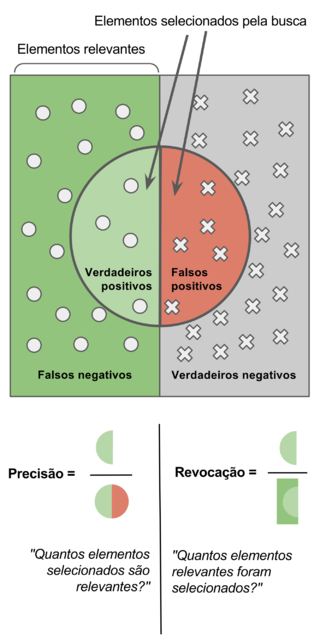
\includegraphics[width=\columnwidth]{Imagens/Precisão_e_revocação.png}
        \caption{Ilustração das métricas de precisão e revocação.}
    \end{minipage}%
    \begin{minipage}{0.5\textwidth}
        \includegraphics[width=\columnwidth]{Imagens/matrix_confusão.png}
        \begin{equation} P = \frac{vp}{vp + vp} \end{equation}
        \begin{equation}R = \frac{vp}{vp + fp}\end{equation}
        \begin{equation}F_\beta = (1+\beta^2) \times \frac {P \times R}{\beta^2 P + R}\end{equation}
        \begin{equation}F_2 = 5 \times \frac {P \times R}{5 P + R}\end{equation}
        \caption{Matriz Confusão, Equações de Precisão, revocação, $F_\beta$ e $F_2$}        
    \end{minipage}       
    \label{fig:metricas}
\end{figure}

Altas taxas de precisão e revocação mostram que o classificafor está retornando resultados relevantes, com poucos falsos positivos (Precisão) e também retornando a maioria de todos resultados positivos (Revocação) \cite{hastie01statisticallearning}. Um sistema com alta revocação e baixa precisão retorna muitos resultados, mas muitos incorretos, enquanto que um com alta precisão e baixa recisão retorna na maioria corretos, mas poucos resultados.

A métrica $F_\beta$ é uma média harmônica entre precisão e revocação, portanto sumariza o compromisso entre esses dois indices  e pesa a importância de cada um a partir de $\beta$.

Podemos comparar métricas e módelos a partir do chamado classificador ingênuo, que atribui a probabilidade de uma classe ser positiva apenas pela frequência de positivos de tal classe no conjunto de dados:

\begin{equation}
    ProbClassIng(X|y=1) = \frac{P}{P + N}
\end{equation}

Em um conjunto de dados muito desbalanceado, métrica de acurácia é pouco capaz de refletir o quão a performance de um modelo é superior ao classificador ingênuo, pois possuem acurácias próximas. Enquanto Precisão-Revocação e métrica $F_2$ é capaz de melhor diferenciar do classificador ingênuo e é capaz de avaliar o o índice de revocação.

Um classificador que retorna a probabilidade de pertencimento de cada classe pode classificar tal classe como positiva ou não ao se comparar com determinado limiar.

A curva precisão-revocação ilustra a relação de compromisso entre os dois indices para diferentes limiares. Uma área grande abaixo da curva representa ambos alta precisão e revocação para muitos limiares diferentes. Do contrário, uma área abaixo da curva \footnote[1]{Area under the curve - AUC} representa que independente do limiar escolhido para o classificador, apresentará baixa precisão e revocação.

Outra métrica para avaliação de classificadores é a curva COR \footnote[2]{Comumente chamada de ROC - Receive Operator Characteristic}, contudo apresenta resultados otimistas para conjuntos de dados balanceados, assim como a acurácia.

Para ambas curvas PR e ROC, um modelo é qualitativamente bom quanto mais performatico for em comparação com o classificador ingênuo, que escolhe classifica com a probabilidade da frequência daquela classe.

\subsection{Função de perda}\label{sec:cap2_fucao_de_perda}

Como métricas de perda para tarefas de classificação, podem ser utilizadas por exemplo, a entropia cruzada, dada por:

Otimizadores possuem como objetivo ajustar pesos de uma função de custo de forma a minimizar ou maximizar tal custo. Para quantificar o custo são utilizadas métricas de perda. Dentre elas, as funções de custos ideais para classificação binária multiclasses e multirótulos temos a entropia binária cruzada, definida por 
$$ECB(y_c) = -\sum_{c=0}^{M} y_c \times log(\hat{y_c})$$
sendo $p(\hat{y_c})$ a probabilidade 

Para conjuntos de dados muito desbalanceados, pode-se mitigar o sobre-ajuste da classe dominante utilizando BCE com pesos do inverso da frequência das classes:
$$ C_i = \frac{FN}{VP_i} $$
$$ECB(y_c) = -\sum_{c=0}^{M} C_i \times y_c \times log(\hat{y_c})$$


Outra solução para mitigar o mesmo problema é a função de perda focal. Consiste de uma ECB penalizando exponencialmente por um peso gama as classificações com probabilidades altas.

$$Focal(y_c) = -\sum_{c=0}^{M} (1-C_i \times y_c \times log(\hat{y_c})$$

\subsection{Redes Neurais Artificiais}\label{sec:Cap2_redes_neurais}

O termo redes neurais embarca uma grande classe de modelos e métodos de aprendizados. O modelo mais simples, também podendo ser chamado rede de camada oculta única de perceptrons. Já o  perceptron é a célula de uma rede neural. Se trata de um modelo matemático análogo a um neurônio. Possui um vetor de entradas e sobre essas entradas é aplicada uma combinação linear utilizando os pesos sobre cada entrada. O resultado de tal operação por sua vez passa por uma função de ativação que resulta numa saída binária de classificação do perceptron. Dessa forma, ao se otimizar os pesos e função de ativação a determinadas amostras de treino e suas respectivas saídas rotuladas, podemos criar um classificador linear simples, caso seja um problema linearmente separável. Portanto o processo de treinamento de uma rede neural se trata de otimizar os pesos dos neurônios. 
Uma etapa importante dos ajustes dos pesos é a retro-propagação de erro\footnote{Frequentemente citada como \textit{Backpropagation}} que é um algoritmo que otimiza os pesos da camada oculta~\cite{hastie01statisticallearning}. 

% TODO: Trocar por sigmoid classificação para muitas classes
Para classificações multi-classes e multi-rótulos, isto é, uma amostra pode pertencer a mais de uma classe simultaneamente, são utilizadas camadas de saída que implementam normalização para selecionar a probabilidade de cada classe.

Temos como exemplo a camada de ativação \textit{Sigmoid}: 


\begin{figure}[!ht]
    \centering
    \begin{minipage}[c]{0.4\textwidth}
        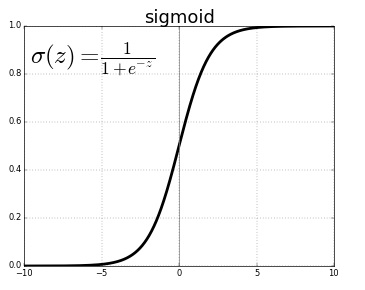
\includegraphics[width=\columnwidth]{Imagens/sigmoid-activation-function.jpg}
        \caption{Ilustração das métricas de precisão e revocação.}
    \end{minipage}%
    \begin{minipage}{0.5\textwidth}
        \begin{equation} Sigmoid(x) = \sigma(x) = \frac{1} {1+ exp(-x)}\end{equation}
        \caption{Exemplo de função de ativação: sigmoid}     
    \end{minipage}       
    \label{fig:sigmoid}
\end{figure}


\begin{figure}[!ht]
    \centering
        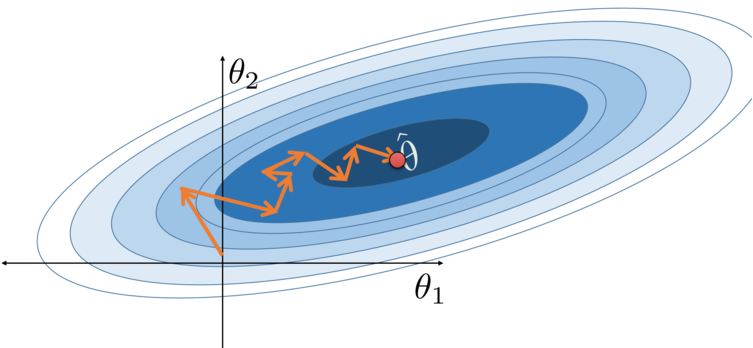
\includegraphics[width=0.47\columnwidth]{Imagens/stochastic_gradient_descent.PNG}
    \caption{Exemplo de algorítimo de otimização: gradiente descendente estocástico. }
    \label{fig:SGD}
\end{figure}






\begin{figure}[!ht]
    \centering
    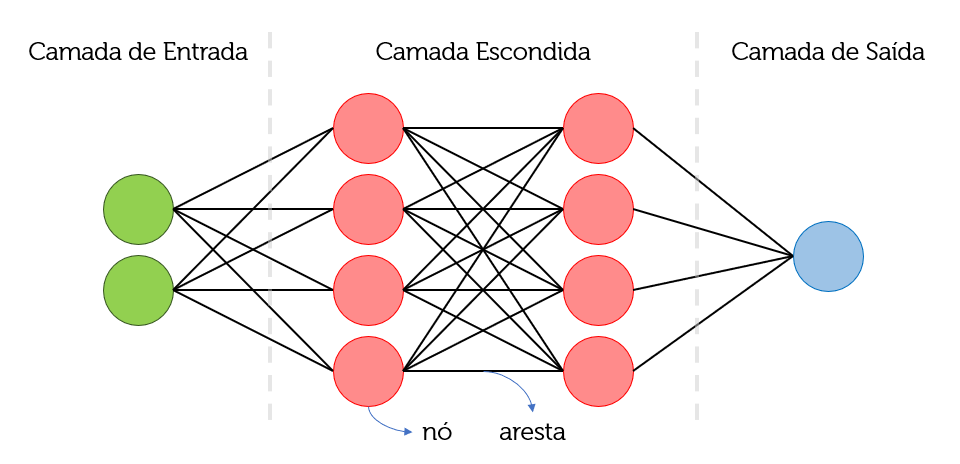
\includegraphics[width=0.6\columnwidth]{
        Imagens/RedeNeural.PNG
    }
    \caption{Exemplo de uma rede de perceptrons de multiplas camadas - MLP.}
    \label{fig:ann}
\end{figure}
\subsection{Redes Neurais Artificiais Profundas}\label{sec:Cap2_redes_neurais_profundas}
O termo redes neurais profundas e o aprendizado profundo, ou comumente chamado de \textit{deep learning}, se refere a redes neurais artificiais com múltiplas camadas ocultas. Foram uma das tecnologias maior desenvolvidas nos últimos anos, e se tornaram cada vez mais popular. Devido a sua superior \textit{performance} em extração de características, teve sucesso por distintos domínios, como visão computacional, reconhecimento de fala, processamento natural de linguagem e em big data.

Um dos riscos envolvendo o treinamento de redes neurais profundas é o problema de \textit{overfiting}\footnote{Sobre-ajuste}. Se trata de quando o modelo é treinado e de forma a gerar uma função próxima demais aos dados de treino, e perdem generalidade, falhando em predições em dados fora do conjunto de treino. Para mitigar o surgimento de \textit{overfiting} durante o treino, são utilizadas técnicas de regularização. Consistem em adicionar penalidade à complexidade do modelo, de forma que o treino otimize para se tornar uma função genérica. Dentre as técnicas de regularização possíveis de DNNs\footnote{\textit{Deep Neural Networks}}, podemos citar o \textit{Dropout, Dropconnect e pruning}, que consistem em respectivamente a remoção, adição de conexão entre neurônios e remoção de neurônios~\cite{hastie01statisticallearning}.


\subsection{Redes Neurais Convolucionais}\label{sec:Cap2_redes_neurais_convolucionais}
Uma arquitetura clássica é a rede neural convolucional (CNN\footnote{\textit{Convolutional Neural Network}}), que utiliza convoluções para extrair características de uma imagem entre cada camada de filtros. Também possui camadas de \textit{pooling}, não lineares e camadas completamente conectadas~\cite{8308186}. Uma dos pressupostos das \textit{CNNs} é os filtros serem indiferentes a translações das características na imagem, possibilitando assim uma eficiente extração de características para composição e identificação da imagem.


Em 2012 o modelo de CNN AlexNet ultrapassou em performance os modelos do estado da arte em uma grande margem. Dois fatores promoveram tal degrau de evolução: a disponibilidade de grandes datasets\footnote{Conjunto de dados} como o ImageNet e a comoditização de placas gráficas, que promoveram significativamente mais poder computacional para treino, já que são aceleradores de operações vetorizadas e sobre matrizes. Dessa forma, desde 2012 CNNs se tornaram o modelo padrão para tarefas de visão computacional \cite{alom2018history}.

A maior vantagem dos modelos CNN em comparação com os métodos anteriores era de ser capaz de ser treinados ponta a ponta, sem a necessidade de criação de filtros ou a criação manual de extratores de características visuais. Também possuem duas importantes propriedades como invariância translacional, isto é, o sistema produz a mesma resposta independente de translação; e campo receptivo restrito, o que significa que neurônios das primeiras camadas capturam detalhes finos e locais.
\begin{figure}[!ht]
    \centering
    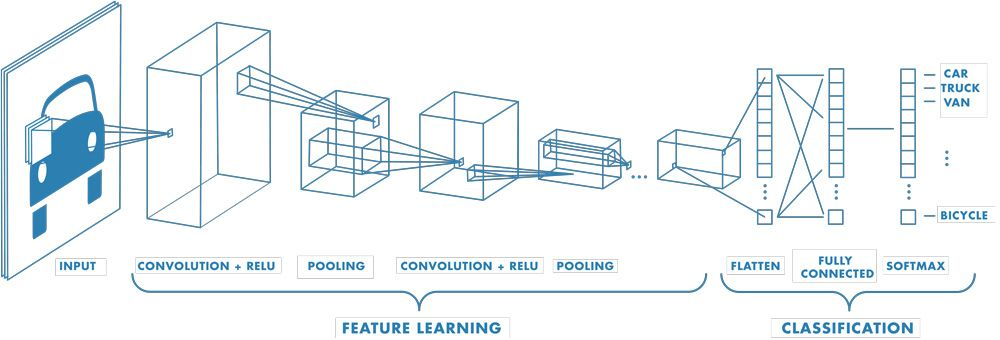
\includegraphics[width=0.95\columnwidth]{
        Imagens/CNN_mathworks.jpg
    }
    \caption{Arquitetura de uma rede convolucional. Filtros extratores de características são aplicados em diferentes resoluções e campos visuais. A saída de cada imagem convoluta alimenta a próxima camada. As ultimas camadas completamente conectadas realizam a classificação.}
    \label{fig:cnn}
\end{figure}

\begin{figure}[!ht]
    \centering
    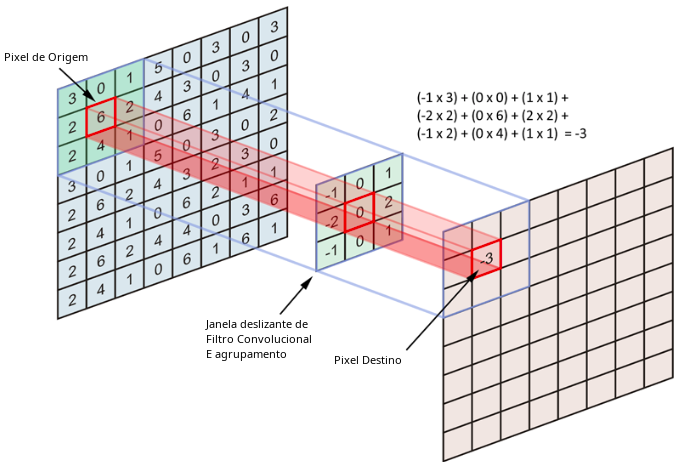
\includegraphics[width=0.6\columnwidth]{
        Imagens/operacao_conv.png
    }
    \caption{
 Filtro convolucional que aplica uma janela deslizante aplicando operação de convolução e pooling.  
        % --- Source: https://towardsdatascience.com/applied-deep-learning-part-4-convolutional-neural-networks-584bc134c1e2
    }
    \label{fig:conv}
\end{figure}






%\subsection{\textit{ResNet}}\label{sec:Cap2_ResNet}
% TODO Resnet

\subsection{\textit{O problema de rotulagem e variabilidade de amostras de treino}}\label{sec:Cap2_rotulagem}

Um dos principais desafios envolvido o treino de \textit{CNNs} aplicado a sensoriamento remoto é representar um estado de características que cubram as variações fotográficas, tanto em características do sensor, como variações da imagem no dia, clima, estação e plataforma da câmera o que se torna uma tarefa difícil. Para uma localização efetiva, o modelo deve ser robusto a todas essas variações, que requer um grande conjunto de treino que cobre boa parte das diversas condições possíveis. Tal conjunto de dados não é disponível e nem viável de obter, pois se trata um volume muito grande de amostras. Tais limitações levam a necessitar o desenvolvimento de algorítimos que aprendem seletivamente para que o poder computacional seja utilizado eficientemente, bem como reutilizar conhecimento prévio e evitar treinamento redundante~\cite{rostami2019learning}.  Dentre as técnicas utilizadas para implementar esses modelos mais eficientes, temos como exemplo o aprendizado supervisionado fraco, e a transferência de aprendizado.

\subsection{\textit{Aprendizado semi-supervisionado}}\label{sec:Cap2_semisup}

As técnicas de aprendizado semi-supervisionado consistem em treinar um modelo com apenas um conjunto reduzido de amostras rotuladas de treino, e as demais amostras serem não supervisionadas. As demais amostras de treino podem ser utilizadas, por exemplo, agrupando-as com as amostras rotuladas e classificando-as como a amostra mais próxima, como apresenta o trabalho de~\cite{Sanches2003}. Outras propostas envolvem~\textit{data augmentation}\footnote{Aumento de dados}, que consistem em gerar um conjunto de treino maior, dados as amostras de treino disponíveis.

\subsection{\textit{Transferência de aprendizado}}\label{sec:Cap2_transfer}

Já técnicas de transferência de aprendizado\footnote{Comumente citado como Transfer Learning}, ou \textit{few shots learning}, consistem em redes treinadas para um conjunto limitado de testes~\cite{rostami2019learning}
e reutilizam esse conhecimento através de diferentes domínios, tarefas ou agentes. Consistem primariamente de um problema origem e um problema objetivo e como podemos suceder em transferir conhecimento dado o problema origem. A abordagem de transferência de conhecimento se inspira em replicar a habilidade dos humanos em que é possível transferir conhecimento de experiências passadas para lidar com tarefas com poucas amostras rotuladas. Este fato inspirou em representar dados de diferentes problemas de aprendizado de máquina em um espaço embutido onde as representações utilizam de diversas relações entre diferentes domínios de conhecimentos e tarefas. Uma implementação encontrada na literatura, proposta em~\cite{rostami2019learning}, consistiu de transplantar a camada de características de uma CNN derivada do domínio de origem para inicializar outra rede, do domínio objetivo, composta por uma camada final fortemente conectada. Assim foi aproveitada as primeiras camadas e a rede foi trenada para o domínio objetivo com uma quantidade menor de amostras.


\section{Transformer Visual}\label{sec:Cap2_transformer_visual}


Temos que a arquitetura de CNNs em si é projetada especificamente para imagens e podem ser computacionalmente onerosas, dessa forma podendo não escalar ou generalizar o suficiente para modelos multimodais. Diante dessas limitações, foram pesquisados modelos que possam escalar e serem agnósticos em quesito de domínios de aplicação. Nessa direção que em \cite{dosovitskiy2020image} é criado o\textit{Transformer} Visual ou ViT \footnote{\textit{Vision Transformer}}, uma arquitetura modelo de visão baseado na possibilidade da utilização da arquitetura Transformer, originalmente utilizada para tarefas baseadas em texto, para tarefas de visão computacional.

O ViT representa uma imagem de entrada como uma sequencia de recortes de imagem, similarmente a uma sequencia de representações de palavras quando aplicado \textit{transformers} para texto, e diretamente predizendo a classe de rótulo da imagem. Tal arquitetura e suas variações apresentaram excelente performance, superando a performance de CNNs até então estado-da-arte, a ResNet, consumindo até um quarto de recursos computacionais.


O\textit{transformer}original recebe como entrada uma sequencia de palavras, que então usa para classificação, tradução ou outras tarefas de processamento natural de linguagem. Para o ViT, em \cite{dosovitskiy2020image} foram aplicadas poucas modificações, de forma a mesma arquitetura ser aplicada a imagens em vez de palavras, e assim observar como o modelo aprende por si próprio.

\begin{figure}[!ht]
    \centering
    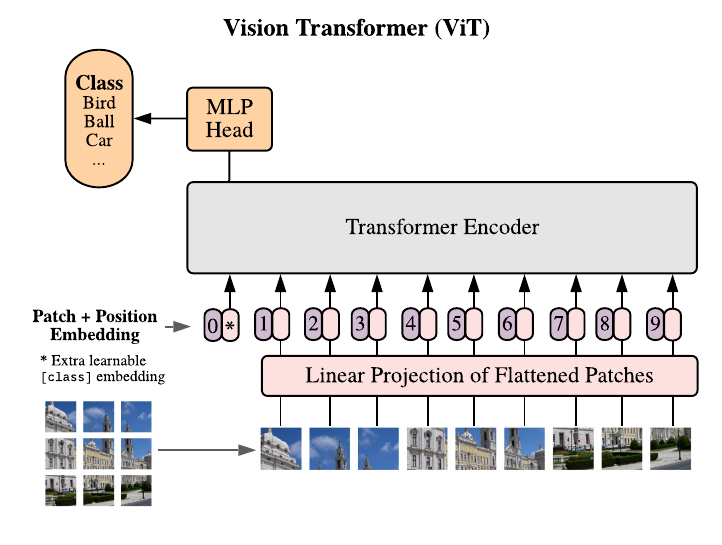
\includegraphics[width=0.65\columnwidth]{
        Imagens/vit.png
    }
    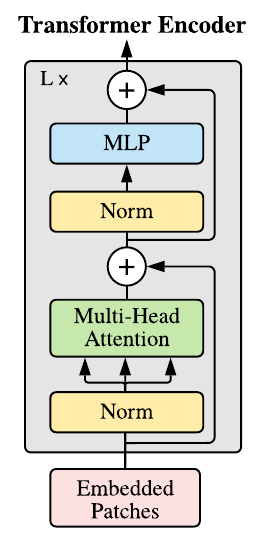
\includegraphics[width=0.34\columnwidth]{
        Imagens/encoder.png
    }
    \caption{O ViT divide uma imagem em uma grade de recortes quadrados, cada fragmento é achatado em um vetor único contendo todos canais de todos os pixeis, e projetando-os em uma dimensão de entrada desejada, alimentando a camada de múltiplos encoders em paralelo. \cite{dosovitskiy2020image}}
    \label{fig:vit}
\end{figure}


\subsection{\textit{Arquitetura do \textit{transformer} visual}}\label{sec:Cap2_vit}

% Mecanismo de atenção
% 

O \textit{encoder transformer} é composto por:
\begin{itemize}
    \item Camada de múltipla cabeças de atenção (MSP): Esta camada concatena todas as saídas de atenção linearmente para a dimensão correta. As várias cabeças de atenção ajudam a treinar local e globalmente dependências em uma imagem.
    \item Camada de múltiplas (MLP) camadas de perceptrons: Contem um MLP de duas camadas com função de ativação GELU (Unidade de erro linear Gaussiano)
    \item Camada de normalização (LN): Adicionada antes de cada bloco e normaliza os pesos dentro de uma mesma camada.
    \item Saltos de conexão: somam a saída de blocos a entrada. Desempenha papel de auxiliar a convergência da otimização do gradiente descendente e explosão de gradientes.
\end{itemize}

A MSP é o núcleo do \textit{encoder}\footnote{Codificador} implementa o mecanismo de auto atenção. Consiste em relacionar diferentes posições de uma única sequência para se computar uma representação desta sequencia \cite{AttentionIsAllYouNeed}.

%\begin{figure}[!ht]
%    \centering
%    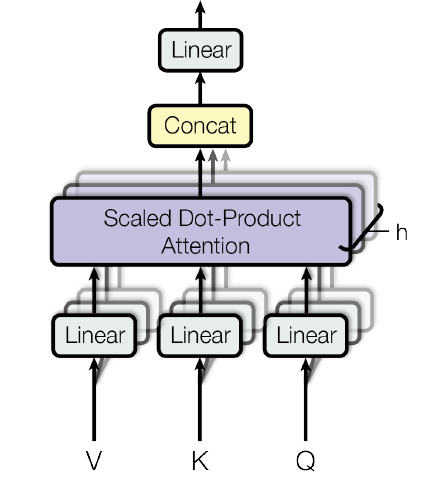
\includegraphics[width=0.4\columnwidth]{
%        Imagens/Multi-Head Attention.png
%    }
%    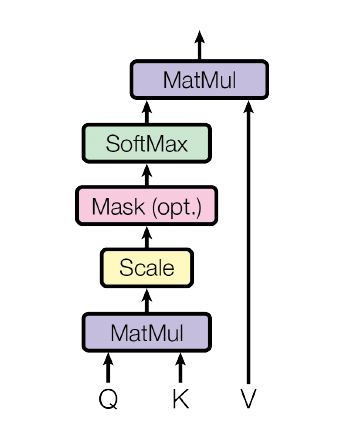
\includegraphics[width=0.4\columnwidth]{
%        Imagens/Scaled Dot-Product Attention.png
%    }
%    \caption{Exemplo de uma rede convolucional. Filtros são aplicados em diferentes resoluções. A saida de cada imagem convoluída alimenta a próxima camada.}
%    \label{fig:attention}
%\end{figure}

% https://towardsdatascience.com/transformers-explained-visually-part-3-multi-head-attention-deep-dive-1c1ff1024853



\begin{figure}[!ht]
    \centering
    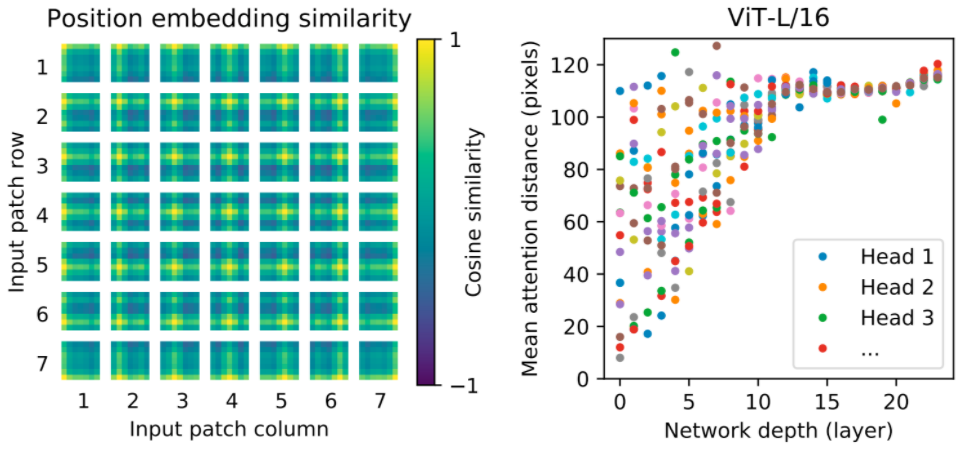
\includegraphics[width=0.9\columnwidth]{
        Imagens/ViTVisualization.png
    }
    \caption{
        Esquerda: ViT aprende a estrutura de grade via representações de posição. Direita: Camadas inferiores do ViT contem ambas características locais e globais, o quão mais profundas as camadas, mais globais as características.\cite{dosovitskiy2020image}
        }
    \label{fig:ViTVisualization}
\end{figure}


É possível observar como o modelo aprende ao visualizar alguns comportamentos internos. Ao observar as representações de posição, que são os parâmetros do modelo que aprendem a codificar a representação relativa dos recortes, encontramos que o ViT é capaz de reproduzir intuitivamente uma estrutura de imagem. Cada representação de posição é mais similar a outras da mesma coluna e linha, indicando que o modelo recuperou a estrutura de grade das imagens originais. Em segundo lugar, examinando a distancia espacial média entre elementos para cada bloco \textit{transformer}. Em camadas mais profundas, apenas características globais são utilizadas, ou seja grandes distâncias de atenção. Enquanto que camadas mais rasas capturam ambas características globais e locais, indicado por uma faixa grande de atenção. Em contraste apenas características locais são presentes nas camadas superficiais das CNNs. Estes experimentos indicam que ViT aprendem características codificadas manualmente nas CNNs, como percepção da estrutura de grade. E principalmente revela que tais modelos são livres para aprender padrões mais genéricos, como mistura de características globais e locais, dessa forma contribuindo para generalização~\cite{dosovitskiy2020image}.
 

\begin{figure}[!ht]
    \centering
    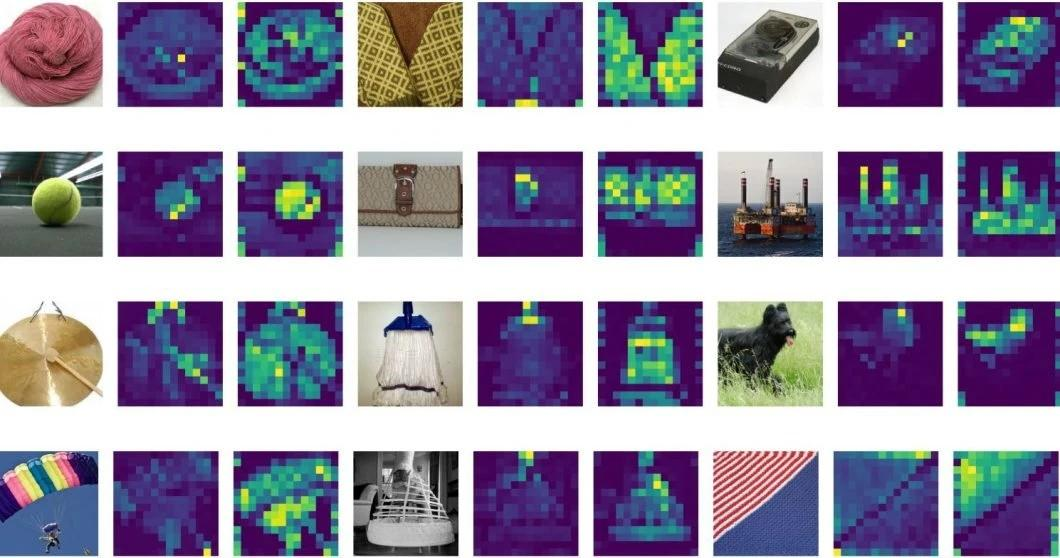
\includegraphics[width=\columnwidth]{
        Imagens/visualizing-attention-vit.jpg
    }
    \caption{
O modelo lida com as regiões que são semanticamente relevantes para classificação. \cite{ViTvsResNets}
        }
    \label{fig:ViTVisualizationAttention}
\end{figure}



\section{Trabalhos anteriores}\label{sec:Cap2_revisao_literatura}

\subsection{Problema de detecção de mudanças em minas de menor escala}\label{sec:Cap2_deteccao_mudanca}

Em \cite{rs14071746} foi gerado um \textit{dataset}\footnote{Conjunto de dados} para detecção de mudanças e de mineração de ouro em menor escala. Com os dados rotulados, foram testadas abordagens supervisionadas e semi-supervisionadas e extratores de características para encontrar um melhor modelo detector de mudanças. Obtiveram o melhor modelo baseado no método E-ReCNN, utilizando seis canais e treino supervisionado, com score f1 de $0.88\pm0.05$.

\subsection{Classificação de minas e represas}\label{sec:Cap2_minas_represa_classificacao}

O problema de classificação para detecção em sensoriamento remoto, utilizando aprendizado profundo foi explorado em ~\cite{s20236936}, utilizando imagens multiespectrais do satélite \textit{Sentinel-2}. Consistiu em treinar um modelo baseado em CNN para identificar em recortes da imagem qual classe pertence.

\subsection{Pré-treino de \textit{transformers} visuais para sensoriamento remoto}\label{sec:Cap2_million}

Para a aplicação de sensoriamento remoto temos trabalhos~\cite{wang2022empirical} que demonstram a aplicação de transferência de aprendizado e redes pré-treinadas utilizando ViT estado-da-arte. Utilizou-se o \textit{dataset} MillionAID, que é o maior \textit{dataset} datado até agora para sensoriamento remoto. Contem mais de um milhão de imagens sem sobreposição, com múltiplas visões temporais para a mesma cena, de canais apenas RGB. Possui uma árvore de classificação com 51 folhas, de cenas de terras de: agricultura, comercial, industrial, serviço público, industrial, transporte, regiões com água e regiões inutilizadas. Cada Folha possui 2.000~45,000 imagens. Foram obtidas pelo \textit{software Google Earth}, que possui uma diversidade de sensores, resultando em diferente resoluções, desde 50cm à 150m. E tamanhos de imagem de 10k pixeis até 900 mega pixeis.
O autor pode concluir que a transferência de aprendizado foi eficaz para posteriores finetune\footnote{Ajuste fino.}.

\subsection{Transformer Swin}\label{sec:Cap2_Swin}

Em~\cite{} foi proposto uma arquitetura de transformer visual com melhorias capazes de reduzir o custo computacional do calculo de atenção entre cada recorte da imagem de entrada. Este trabalho aponta que a ordem de complexidade do ViT clássico é O(n²), sendo n o número de retalhos, já que é calculado a métrica de atenção entre cada retalho com todos os outros demais. Com isso, torna caro o treino para maiores resoluções ou granularidade de detalhes. A arquitetura SWIN, ou \textit{Shifted Window} se baseia em uma disposição hierárquica de transformers, sendo que nas camadas mais baixas, coletam atenção apenas localmente e não com todo restante da imagem. Dessa forma o custo se torna aproximadamente linear. 


\begin{figure}[!ht]
    \centering
    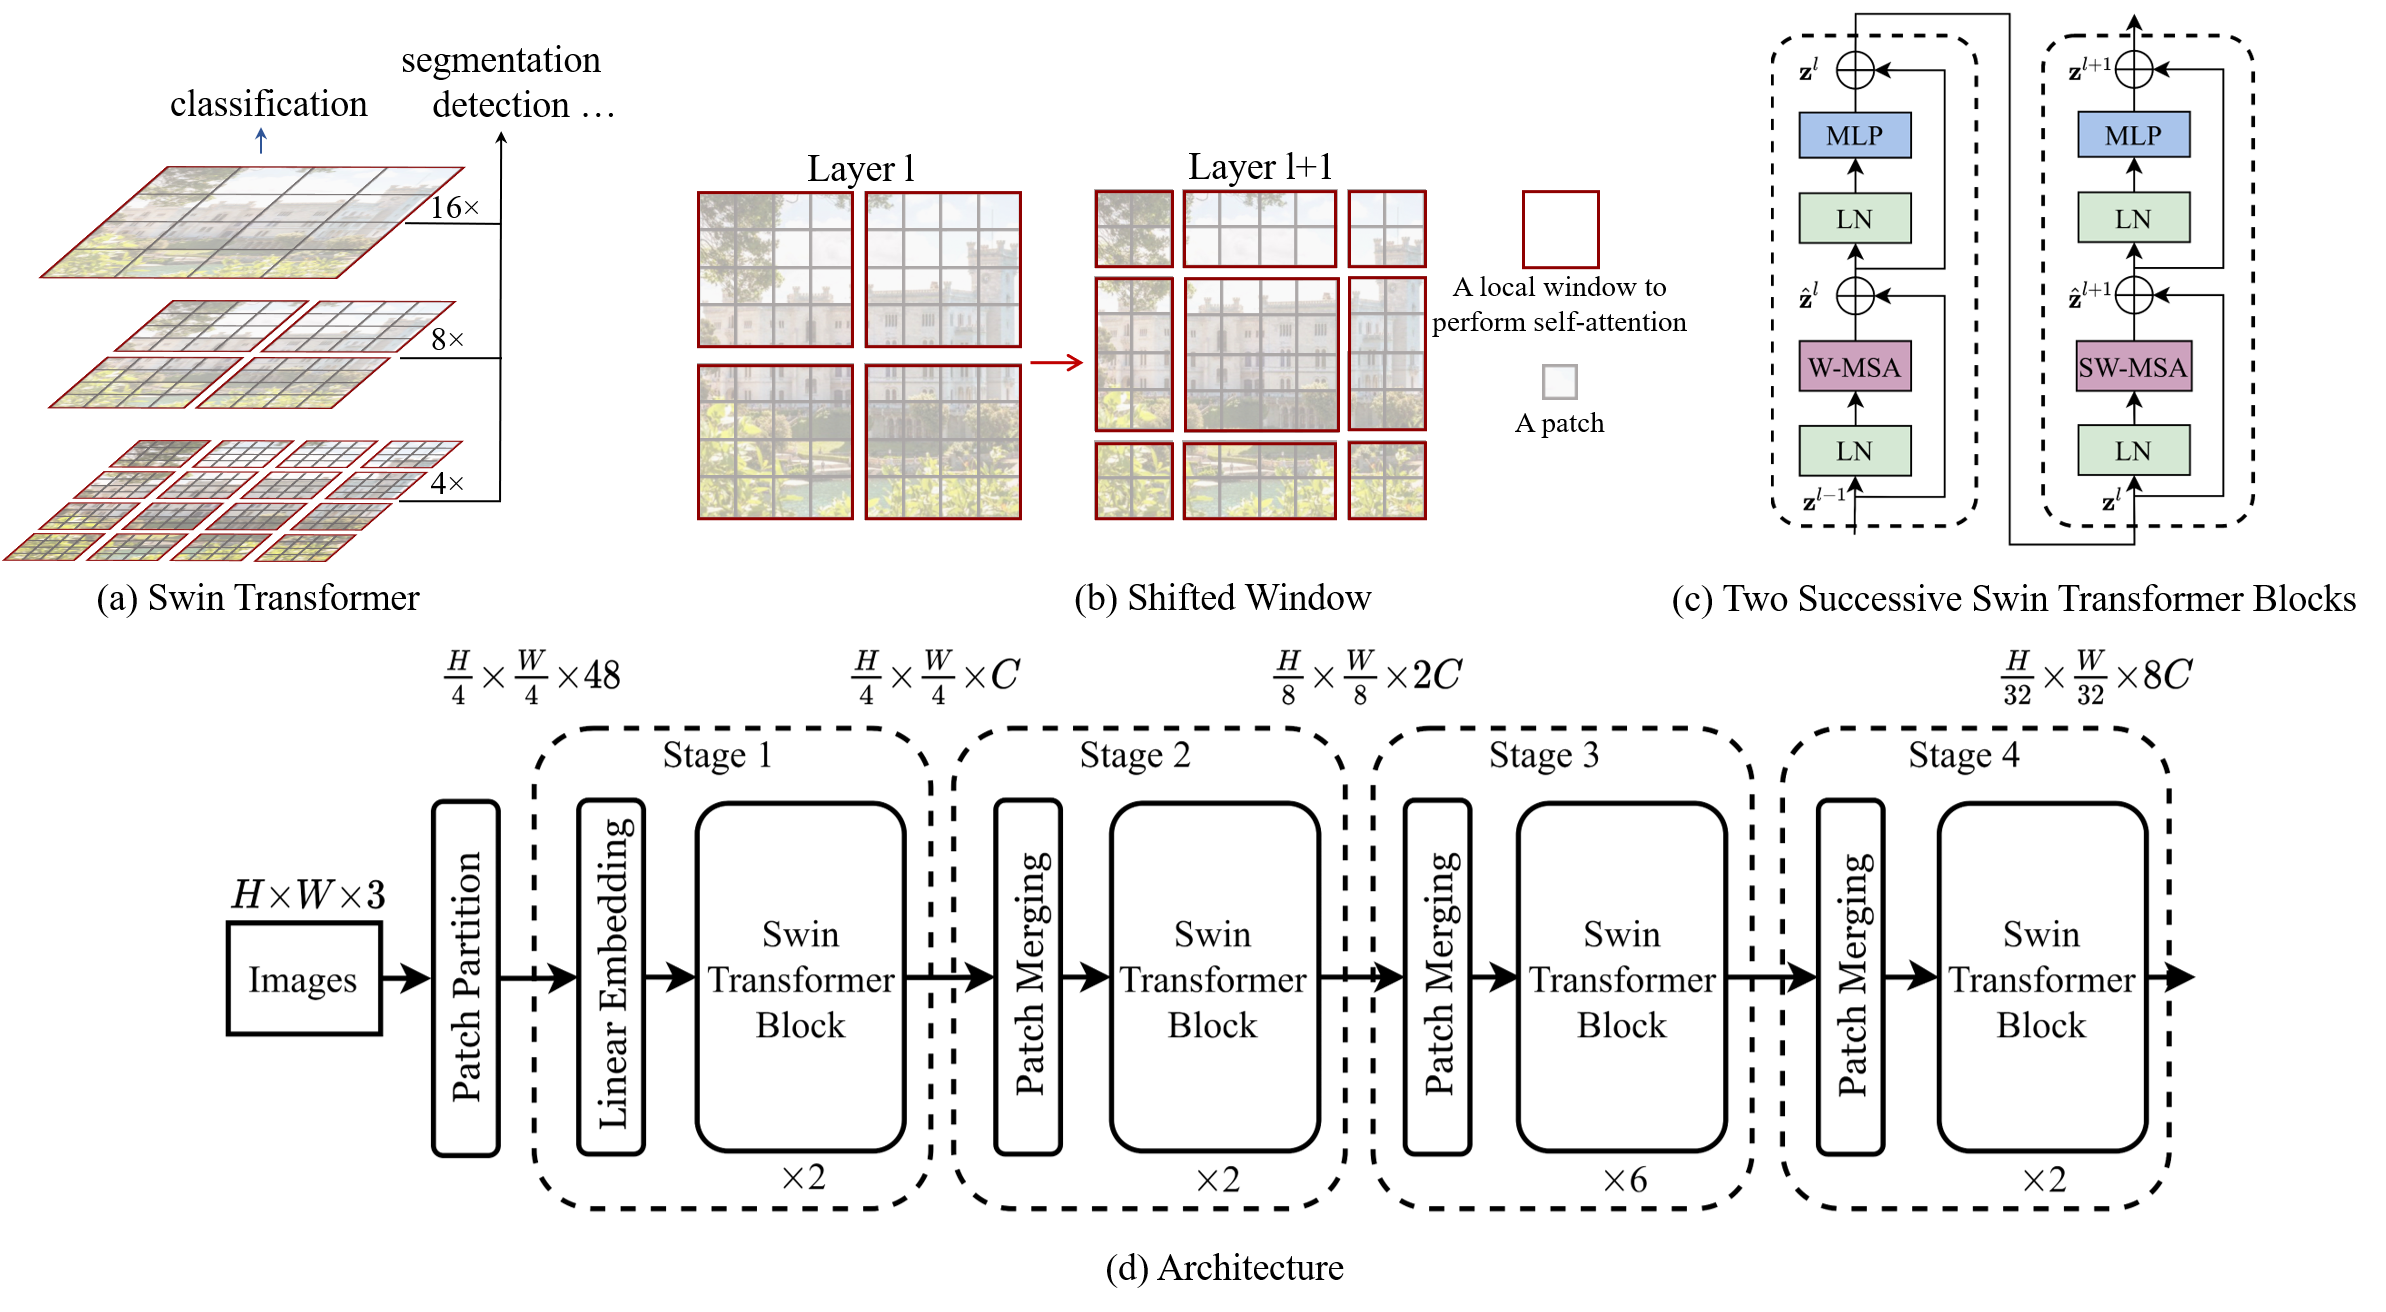
\includegraphics[width=\columnwidth]{Imagens/arquitetura swin.png}
    \caption{Arquitetura swin ~\cite{liu2022swin}}
    \label{fig:SWIN-arquitetura}
\end{figure}

dois blocos swin sucessivos.png

\subsection{ForestViT Modelo de classificação de desmatamento}\label{sec:Cap2_ForestViT}

Em~\cite{9701667} foi proposto um classificador multiclasses baseado na arquitetura de \textit{transformers} visual. Os resultados também foram comparados com modelos baseados em CNN estabelecidos, como Resnet e VGG. 


%We utilize a dataset (URL: https://www.kaggle.com/c/planet-understanding-the-amazon-from-space/data) published in a Kaggle competition (by Planet company), containing coarse-resolution imagery data from satellites with varying spatial resolution characteristics, i.e., the imagery has a ground-sample distance (GSD) of 3.7 m and an orthorectified pixel size of 3 m. The data comes from Planet’s Flock tow satellites in both Sun-synchronous and ISS orbits and was collected in the time interval between January 1, 2016, and February 1, 2017. All of the images are derived from the Amazon basin. Mangrove deforestation in the Amazon forest is an intense phenomenon, and a plethora of factors that contribute to deforestation is observed there. Each entry contains imagery data in RGB plus the infrared band in geo-referenced.tiff format. In our experiment, the images are classified into 14 classes and the labels are broken into three groups: atmospheric conditions, common land cover/land use phenomena, and rare land cover/land use phenomena (see Fig. 3). Here, each entry is assigned to one or more classes.


% Abstract: Monitoring changes within the land surface and open water bodies is critical for natural resource management, conservation, and environmental policy. While the use of satellite imagery for these purposes is common, fine-scale change detection can be a technical challenge. Difficulties arise from variable atmospheric conditions and the problem of assigning pixels to individual objects. We examined the degree to which two machine learning approaches can better characterize change detection in the context of a current conservation challenge, artisanal small-scale gold mining (ASGM). We obtained Sentinel-2 imagery and consulted with domain experts to construct an open-source labeled land-cover change dataset. The focus of this dataset is the Madre de Dios (MDD) region in Peru, a hotspot of ASGM activity. We also generated datasets of active ASGM areas in other countries (Venezuela, Indonesia, and Myanmar) for out-of-sample testing. With these labeled data, we utilized a supervised (E-ReCNN) and semi-supervised (SVM-STV) approach to study binary and multi-class change within mining ponds in the MDD region. Additionally, we tested how the inclusion of multiple channels, histogram matching, and La*b* color metrics improved performance of the models and reduced the influence of atmospheric effects. Empirical results show that the supervised E-ReCNN method on 6-Channel histogram-matched images generated the most accurate detection of change not only in the focal region (Kappa: 0,92(±0.04), Jaccard: 0,88(±0.07), F1:0.88(±0.05)) but also in the out-of-sample prediction regions (Kappa: 0,90(±0.03), Jaccard: 0,84(±0.04), and F1: 0,77(±0.04)). While semi-supervised methods did not perform as accurately on 6- or 10-channel imagery, histogram matching and the inclusion of La*b* metrics generated accurate results with low memory and resource costs. These results show that E-ReCNN is capable of accurately detecting specific and object-oriented environmental changes related to ASGM. E-ReCNN is scalable to areas outside the focal area and is a method of change detection that can be extended to other forms of land-use modification.



% In this work we present BrazilDAM, a novel public dataset based on Sentinel-2 and Landsat-8 satellite images covering all tailings dams cataloged by the Brazilian National Mining Agency (ANM). The dataset was built using georeferenced images from 769 dams, recorded between 2016 and 2019. The time series were processed in order to produce cloud free images. The dams contain mining waste from different ore categories and have highly varying shapes, areas and volumes, making BrazilDAM particularly interesting and challenging to be used in machine learning benchmarks. The original catalog contains, besides the dam coordinates, information about: the main ore, constructive method, risk category, and associated potential damage. To evaluate BrazilDAM's predictive potential we performed classification essays using state-of-the-art deep Convolutional Neural Network (CNNs). In the experiments, we achieved an average classification accuracy of 94.11% in tailing dam binary classification task. In addition, others four setups of experiments were made using the complementary information from the original catalog, exhaustively exploiting the capacity of the proposed dataset. 


% https://huggingface.co/docs/transformers/model_doc/vit
% https://huggingface.co/blog/fine-tune-vit 
% https://huggingface.co/blog/your-first-ml-project
% https://huggingface.co/blog/accelerate-deepspeed
% https://huggingface.co/blog/fine-tune-vit

% \part{Segunda entrega}
\chapter{Metodologia}
\label{sec:metodologia}
A metodologia para a execução deste trabalho está dividida em três partes, conforme as seções a seguir. A Seção \ref{sec:Cap3_Deteccao} apresenta a definição do algoritmo selecionado para a resolução do problema de identificação de objetos a partir de imagens, e seu desenvolvimento. Adiante, na Seção \ref{sec:Cap3_Controle} é explicado como obter parâmetros do manipulador robótico junto ao desenvolvimento de seu controlador. Por fim, a Seção \ref{sec:Cap3_Simulador} apresenta as estratégias de simulação do sistema a fim de integrar todas as soluções propostas. A Figura \ref{fig:metodologia} ilustra os principais passos da metodologia.

\begin{figure}[h!]
    \centering
    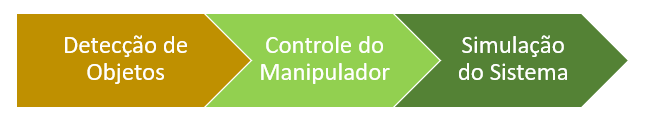
\includegraphics[width=.75\columnwidth]{Imagens/DiagramaMetodologia.PNG}
    \caption{Metodologia com os principais passos utilizados na execução deste trabalho.}
    \label{fig:metodologia}
\end{figure}

%==============================================================
\section{\textit{Detecção de Objetos}}\label{sec:Cap3_Deteccao}

Durante as últimas décadas, foram desenvolvidas muitas tecnologias e \textit{frameworks} voltados para detecção de objetos. Muitos destes são fornecidos de forma paga por empresas do meio, porém existem implementações gratuitas e de qualidade fornecidas por gigantes da indústria tecnológica, e com grande suporte de desenvolvedores independentes. Devido ao suporte e ajuda crescente da comunidade, além da praticidade em suas usabilidades, chegou-se a conclusão que seria mais eficiente a utilização da biblioteca OpenCV \cite{howse2013opencv}, para a captura das imagens, e TensorFlow \cite{tensorFlow}, para tratar a identificação de objetos, ambos com suporte para a linguagem de programação Python.

Em uma primeira etapa, a Subseção \ref{sec:Cap3_D_OpenCV} irá apresentar um método para captura de imagens que serão tratadas eventualmente. A Subseção \ref{sec:Cap3_D_TensorFlow} irá contextualizar brevemente a respeito do \textit{framework} TensorFlow e alguns conceitos teóricos de Redes Neurais. Enquanto que a Subseção \ref{sec:Cap3_D_Modelo} irá apresentar conceitos dos modelos pré-treinados e definir um modelo a ser utilizado a fim de cumprir o propósito deste trabalho.
 
%-------------------------------------------------------------
\subsection{\textit{OpenCV}}\label{sec:Cap3_D_OpenCV}
 
O OpenCV (\textit{Open Source Computer Vision Library}) é uma biblioteca de código aberto que tem foco na visão computacional em tempo real. Ele possui módulos de processamento de imagens e vídeos, e possui uma ampla utilização da comunidade desenvolvedora na utilização de diversas áreas graças a suas ferramentas que permitem filtros, calibração e reconhecimento de padrões. Por mais que ele possa ser utilizado como ferramenta para reconhecimento de objetos em cena, ele foi utilizado neste cenário apenas a captura de imagem em tempo real. Isso se deve a seu processamento ser todo na máquina local, enquanto o TensorFlow possui vantagens que aliviam o custo computacional de todo o processamento.

A biblioteca foi desenvolvida na linguagem de programação C++, porém existe suporte atualmente para outras linguagens, como Python e Java. O OpenCV está em constante manutenção para agregar melhorias de desempenho e novas funcionalidades, sendo sua última versão estável lançada em abril de 2021. Por se tratar de um código aberto, ele pode ser customizável e explorado a fim de garantir uma funcionalidade ou melhoria que se adeque melhor ao projeto. Para este projeto, entretanto, serão utilizadas funções que já estão integradas à biblioteca.

Existem atualmente duas versões da biblioteca, sendo a versão 1.0 lançada em 2006 e a versão 2.0 lançada em 2009. A última versão será utilizada neste trabalho, juntamente com suas funções de captura de vídeo a fim de poder armazenar e tratar os quadros de imagens a serem processados.
 
%-------------------------------------------------------------
\subsection{\textit{Redes Neurais e TensorFlow}}\label{sec:Cap3_D_TensorFlow}

Existem muitos elementos da engenharia que foram mimetizados de elementos da natureza e de seres vivos. Um grande exemplo de uma tecnologia nesse sentido que vem sendo amplamente utilizada, são as chamadas Redes Neurais. Elas são modelos computacionais que se inspiram na funcionalidade dos neurônios para realização de Aprendizado de Máquina, tal como Reconhecimento de Padrões.

Assim como os humanos aprendem a reconhecer coisas na natureza a partir de treinamentos de discernimento, as Redes Neurais passam pelo mesmo processo, realizando uma iteração com ajustes aplicados em seus pesos, a qual é chamada de treinamento. Sua composição é realizada por nós e arestas, que são análogos a neurônios e sinapses, respectivamente.

Inicialmente, alguns dados são percorridos ao longo do sistema para que possam ser gerados informações comparativas. Após essa etapa, o sistema está pronto para receber novos dados para comparar com os já conhecidos, a fim de gerar um resultado da iteração. Dessa forma, as arquiteturas podem ser classificadas como: Camada de Entrada, Camada Escondida ou Intermediária, e Camada de Saída. A primeira está relacionada com a inserção dos padrões apresentados. O processamento de dados ocorrem majoritariamente na Camada Intermediária, onde existe um maior fluxo de arestas e nós. O resultado é disponibilizado na Camada de Saída. O esquemático representando a estrutura pode ser observado na Figura \ref{fig:RedeNeural}.

\begin{figure}[h!]
    \centering
    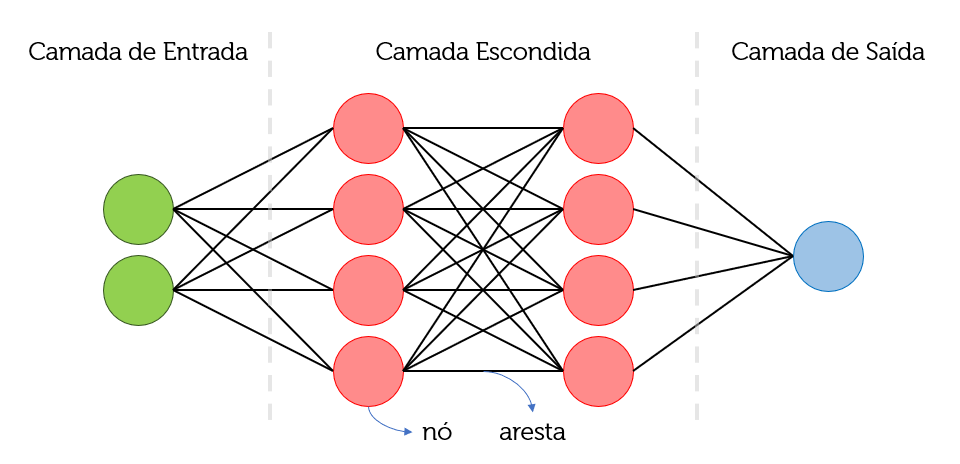
\includegraphics[width=.75\columnwidth]{Imagens/RedeNeural.PNG}
    \caption{Estrutura organizacional de uma Rede Neural.}
    \label{fig:RedeNeural}
\end{figure}

O TensorFlow é um exemplo de ambiente de código aberto para uso de Aprendizado de Máquina que foi desenvolvido pela Google. Ele vem sido bastante utilizado para soluções tecnológicas de muitas empresas nos últimos tempos, como a Coca-Cola \cite{brandt_how_2017}, a GE \cite{polzin_intelligent_2019} e a própria Google \cite{bendersky_google_2021}. Por ser uma aplicação gratuita e de fácil uso de Redes Neurais, e por apresentar uma comunidade ativa e com suporte por parte dos desenvolvedores, o \textit{framework} se tornou uma alternativa agradável para desenvolver e treinar modelos de aprendizado.

A maior vantagem do TensorFlow para este projeto é a sua flexibilidade. Ele foi criado para ser executado em diversas plataformas e sistemas operacionais, sejam estes os tradicionais computadores ou dispositivos móveis. De acordo com o modelo a ser treinado, ele pode ser executado por uma CPU\footnote{CPU: \textit{Central Process Unit}}, uma GPU\footnote{GPU: \textit{Graphics Processing Unit}} ou uma TPU\footnote{TPU: \textit{Tensor Processing Unit}}, esta última sendo uma criação da própria Google para ser utilizada junto ao TensorFlow. A biblioteca permite que execute todo o processamento de forma local, em um computador ou dispositivo móvel, além de permitir um processamento na nuvem, o que se faz bem útil para aqueles que não possuem um hardware potente.


%-------------------------------------------------------------
\subsection{\textit{Modelo pré-treinado}}\label{sec:Cap3_D_Modelo}

Através de um banco de dados, é possível treinar um modelo com o TensorFlow. A Google disponibiliza uma página\footnote{TensorFlow: \url{https://www.tensorflow.org/}} com o suporte para todo o processo, porém a biblioteca também permite a utilização de modelos pré-treinados para que sejam utilizados por outros membros da comunidade desenvolvedora.
% Estes modelos reduzem o tempo desempenhado no projeto e são capazes de apresentar resultados melhores do que se produzidos com outros bancos de dados. Muitos destes modelos são constantemente atualizados para prover melhorias, sendo alguns deles disponibilizados na própria página do TensorFlow.

Neste trabalho foi utilizado como modelo o COCO-SSD. Trata-se de um modelo pré-treinado desenvolvido e envelopado por desenvolvedores do Google capaz de identificar múltiplos objetos diferentes em uma imagem. O modelo consegue identificar 90 objetos diferentes \cite{noauthor_pre-trained_2021} que podem ser encontrados no cotidiano. Seu nome vem da junção de duas siglas: COCO e SSD. COCO (\textit{Common Objects in Context}) é um dataset construído pela Microsoft que foi utilizado para treinamento, sendo disponibilizado gratuitamente com mais de 200 mil imagens. Já SSD (\textit{Single Shot Detector}) é um detector de objetos que é capaz de identificar as diferentes classes de objetos. \cite{forson_understanding_2019}.

\begin{figure}[b!]
\centering
\includegraphics[width=0.7\columnwidth]{Imagens/BoundaryBox.jpeg}
\caption{Caixa delimitadora mínima na utilização do COCO-SSD. \cite{mayes_make_2021}}
\label{fig:cocossd}
\end{figure}

O COCO-SSD é capaz de identidicar diferentes objetos em uma mesma imagem, mesmo que sobrepostos. Para isso, ele cria uma caixa delimitadora mínima que é capaz de envolver o objeto com a menor medida de identificação possível. Além disso, ele identifica um nível de confiabilidade do objeto identificado no topo das caixa a partir de uma porcentagem. Um exemplo pode ser observado na Figura \ref{fig:cocossd}.

% \begin{figure}[b!]
% \centering
% \includegraphics[width=0.7\columnwidth]{src/imgs/BoundaryBox.jpeg}
% \caption{Caixa delimitadora mínima na utilização do COCO-SSD.}
% \label{fig:cocossd}
% \end{figure}

O algoritmo de detecção de objetos do TensorFlow foi incorporado a um \textit{script} desenvolvido para a solução do problema proposto neste trabalho. O \textit{script} tem como entrada a imagem capturada pela câmera e armazenada através de funções disponíveis pelo OpenCV. Como saída, o \textit{script} retorna os vértices das posiçãos onde foram detectadas as pessoas na imagem. Estes dados serão tratados e servirão de base para o posicionamento desejado do efetuador do manipulador robótico.


%===========================================================
\section{\textit{Controle de Manipulador Robótico}}\label{sec:Cap3_Controle}

Os Manipuladores Robóticos são capazes de administrar tarefas com boa precisão, além de automatizar processos. A componente de maior importância em um manipulador é, em muitas vezes, o efetuador, a qual se encontra em um extremo, e é capaz de se movimentar dentro de uma área de trabalho e exercer funções pré-determinadas. Isso pode ser apresentado na Figura \ref{fig:workspace}, a qual a região hachurada representa a área de trabalho em que o efetuador pode operar.

\begin{figure}[h!]
\centering
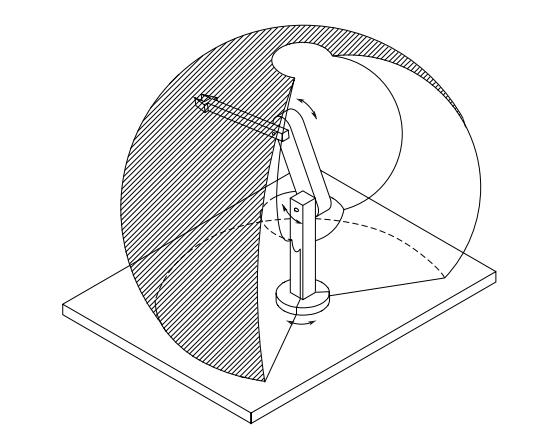
\includegraphics[width=0.7\columnwidth]{Imagens/workspace.PNG}
\caption{Área de trabalho de um Manipulador Robótico. \cite{siciliano2010robotics}}
\label{fig:workspace}
\end{figure}

Em uma primeira etapa, a Subseção \ref{sec:Cap3_Espacial} irá apresentar conceitos importantes que serão utilizados no controle do manipulador. A Subseção \ref{sec:Cap3_CinDir} irá definir métodos utilizados para leitura de pose do manipulador, enquanto a subseção \ref{sec:Cap3_CinDif} irá definir métodos para leitura de velocidade. Por fim, a Subseção \ref{sec:Cap3_ControleCin} irá apresentar técnicas de controle que irão utilizar de dados que foram apresentados na Seção \ref{sec:Cap3_Deteccao}.

%-------------------------------------------------------------
\subsection{\textit{Descrição Espacial}}\label{sec:Cap3_Espacial}

Para compreender o comportamento dos elementos de um manipulador robótico, é necessário saber como eles são descritos dentro de um espaço tridimensional a qual será servirá para localização no espaço real dos objetos. Primeiro, é preciso definir um ponto de origem que seja comum a todos os objetos que serão representados no cenário. Além disso, é necessário definir os eixos $x$, $y$ e $z$, que são ortogonais entre si, e que possuem origem no ponto citado. Esses dados serão úteis para definição de posição e orientação do objeto no cenário.

\begin{figure}[h!]
\centering
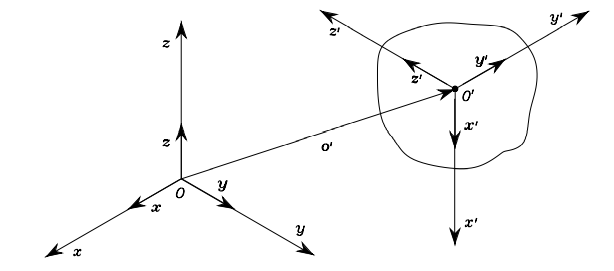
\includegraphics[width=0.7\columnwidth]{Imagens/PosEOri.PNG}
\caption{Posição e orientação de um objeto no cenário. \cite{siciliano2010robotics}}
\label{fig:PoseOri}
\end{figure}

Pode-se perceber pela Figura \ref{fig:PoseOri} que a posição de um objeto na posição do ponto $O'$ pode ser expressa com relação ao ponto e coordenadas de origem como:

\begin{equation}
o' = o'_xx+o'_yy+o'_zz
\label{eq:3_01}
\end{equation}

Uma vez que $o'_x$, $o'_y$ e $o'_z$ são componentes do vetor $o'\in \mathbf{R}^3$, a posição de $O'$ pode ser descrita de acordo com o seguinte vetor (3x1):

\begin{equation}
o' = 
\begin{bmatrix}
o'_x & o'_y & o'_z
\end{bmatrix} ^T
\label{eq:3_02}
\end{equation}

Para descrever a orientação do objeto, é adequado considerar eixos ortogonais que serão deslocados em referência aos eixos da origem. Dessa forma, os eixos podem ser representados pelas seguintes expressões:

\begin{equation}
\begin{matrix}
x' = x'_xx+x'_yy+x'_zz\\
y' = y'_xx+y'_yy+y'_zz\\
z' = z'_xx+z'_yy+z'_zz
\end{matrix}
\label{eq:3_03}
\end{equation}

Descrevendo a Equação \ref{eq:3_03} como um vetor (3x3), é possível obter a matriz de rotação ($Q$) do objeto, que é definida pela Equação \ref{eq:3_04}.

\begin{equation}
Q = 
\begin{bmatrix}
x' & y' & z'
\end{bmatrix}  = 
\begin{bmatrix}
x'_x & y'_x & z'_x \\
x'_y & y'_y & z'_y \\
x'_z & y'_z & z'_z
\end{bmatrix}  = 
\begin{bmatrix}
x'^Tx & y'^Tx & z'^Tx \\
x'^Ty & y'^Ty & z'^Ty \\
x'^Tz & y'^Tz & z'^Tz
\end{bmatrix}
\label{eq:3_04}
\end{equation}

É importante pontuar que, aplicando uma orientação que segue os fundamentos da regra da mão direita, o determinante da matriz será de tal forma que $det(Q) = 1$. A estrutura que compõe a posição e rotação de um objeto dado um determinado tempo, é chamada de referencial – também conhecido como \textit{frame}.

% \begin{figure}[h!]
% \centering
% \includegraphics[width=0.7\columnwidth]{Imagens/DoisPontos.PNG}
% \caption{Vetores de posição dado dois objetos e \textit{referência mundo}.}
% \label{fig:DoisPontos}
% \end{figure}

Quando existe mais de um objeto em um dado cenário, é possível representar os objetos com relação a origem ou com relação entre si. Para isso, define-se o vetor de posição dos vértices como $p_O^D$, sendo $O$ o ponto de origem e $D$ o ponto de destino do vetor. Isso pode ser melhor avaliado na Figura \ref{fig:DoisPontos}. Há técnicas dentro da robótica que utilizam os vetores sempre com relação ao chamado \textit{referência mundo}, que serve de referência universal para todos os objetos do cenário; enquanto outros adotam referências sempre de acordo com o objeto anterior analisado.

\begin{figure}[h!]
\centering
\includegraphics[width=0.7\columnwidth]{Imagens/DoisPontos.PNG}
\caption{Vetores de posição dado dois objetos e \textit{referência mundo}.}
\label{fig:DoisPontos}
\end{figure}

% \begin{figure}[b!]
% \centering
% \includegraphics[width=0.7\columnwidth]{src/imgs/DoisPontos.PNG}
% \caption{Vetores de posição dado dois objetos e \textit{referência mundo}. \cite{siciliano2010robotics}}
% \label{fig:DoisPontos}
% \end{figure}

Uma notação muito comum no campo da robótica é a Matriz de Transformação Homogênea. Com ela, é possível demonstrar a posição e orientação de um objeto dado uma referência. Ela é composta pela matriz de rotação ($Q$), vetor de posição ($p$) e preenchida por valores nulos e unitários para que a matriz possa ser quadrada. Dessa forma, a Matriz de Transformação Homogênea ($H_{4x4}$) pode ser representada pela Equação \ref{eq:3_05}.

\begin{equation}
H_0^1 = 
\begin{bmatrix}
Q_0^1 & p_0^1 \\
0_{1x3} & 1
\end{bmatrix} 
\label{eq:3_05}
\end{equation}

O objeto pode sofrer transformações de rotação e posição, e é necessário definir a leitura da ordem das ações tomadas. Dado um produto $T = R_x(\pi)R_z(\pi/2)$, pode-se ler a transformação da direita para a esquerda, ou da esquerda para a direita. No primeiro cenário, irá ocorrer uma rotação de $\pi/2$ no eizo $z_0$ e depois uma rotação de $\pi$ em $x_0$. No segundo cenário, irá ocorrer uma rotação de $\pi$ no eizo $x_0$ e depois uma rotação de $\pi/2$ em $z_1$. Perccebe-se então que a ordem influencia no estado do \textit{frame} final, sendo o primeiro cenário considerando o \textit{frame 0} como referência, e no segundo, considerando o \textit{frame} anterior.

Com os conceitos de descrição espacial definidos, é possível conhecer mais sobre a Cinemática Direta a fim de obter os dados dos \textit{frames} de um manipulador robótico.

%-------------------------------------------------------------
\subsection{\textit{Cinemática Direta}}\label{sec:Cap3_CinDir}

A Cinemática permite estudar os movimentos dos manipuladores sem a necessidade de tratar força e torque em suas análises. Para este estudo, se usa o conceito de Espaço de Configurações, normalmente denotado por $Q$. Ele é o conjunto de todas as configurações de um sistema, sendo cada configuração um conjunto de coordenadas que permite identificar uma partícula do manipulador no espaço. A configuração é denotada por $q$, e pode ser representada por coordenadas cartesianas, polares, entre outras.

Definindo um \textit{frame} de \textit{referência mundo}, pode-se descrever o estado atual do \textit{frame} do efetuador a partir do deslocamento de juntas prismáticas e/ou rotação de juntas rotativas. É possível definir uma função de Cinemática Direta do frame desejado, sendo esta uma função da configuração $q$, como pode ser observado na Equação \ref{eq:3_06}.

\begin{equation}
T = f(q)
\label{eq:3_06}
\end{equation}

A Convenção de Denavit-Hartenberg é muito utilizada na área da robótica para definir a Cinemática Direta de um manipulador. Ela define regras para criação de referenciais intermediários ao longo do manipulador de forma que facilite a transformação de um referencial de origem – geralmente utilizando o \textit{referencial do mundo} – para um referencial final desejado.

Para isso, é necessário definir alguns conceitos:

\begin{itemize}
\item $elo_i:$ \textit{i}-ésimo elo.
\item $reta_i:$ reta alinhada com o eixo de rotação/translação \textit{i}, afixada ao $elo_i$. 
\item $pontoA_i:$ ponto da $reta_i$ mais próximo de $reta_{i+1}$.
\item $pontoB_i:$ ponto da $reta_{i+1}$ mais próximo de $reta_i$.
\item $frame_i:$ eixo afixado no $elo_i$.
\end{itemize}

Definido os conceitos, é aplicado um método geral para a convenção, sendo $i$ o número da junta analisada no atual momento. Dessa forma, aplica-se a seguinte ordem de ações:

\begin{enumerate}
\item Traçar a $reta_i$ e a $reta_{i+1}$.
\item Encontrar o $pontoA_i$ e o $pontoB_i$.
\item O $frame_{i+1}$ estará centrado no $pontoB_i$.
\item É convencionado que o eixo $z_i$ está alinhado com o eixo de rotação/deslocamento da $reta_i$.
\item Alinha-se o eixo $z_i$ com relação ao próximo eixo de rotação/deslocamento, da $reta_{i+1}$.
\item O eixo $x_i$ tem seu sentido inicial arbitrário.
\item Alinha-se o eixo $x_i$ no sentido de $pontoA_i$ para $pontoB_i$.
\item Aplicando a regra da mão direita, define-se o eixo $y_i$.
\end{enumerate}

Por fim, define-se as variáveis de rotação e trasnalação, sendo estas:

\begin{itemize}
\item $a_i:$ translação no eixo $x$.
\item $\alpha_i:$ rotação no eixo $x$. 
\item $d_i:$ translação no eixo $z$.
\item $\vartheta_i:$ rotação no eixo $z$. 
\end{itemize}

Aplicando as regras acima no braço antropomórfico da Figura \ref{fig:BracoAntro} como exemplo, é possível obter os parâmetros de Denavit-Hartenberg descritos na Tabela \ref{table:3_01}.

\begin{figure}[b!]
\centering
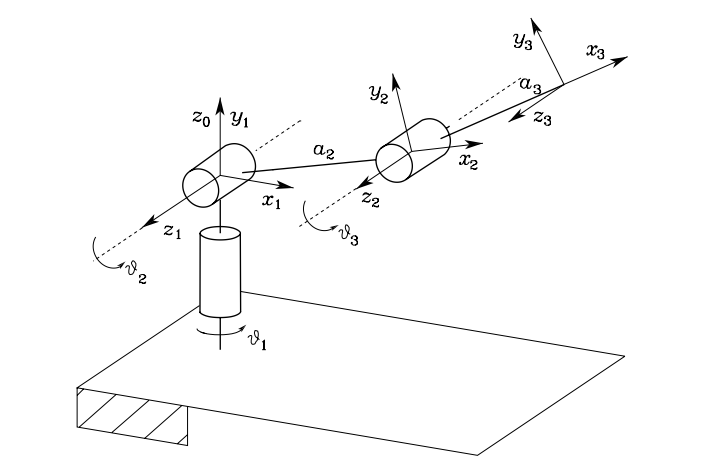
\includegraphics[width=0.7\columnwidth]{Imagens/BracoAntropo.PNG}
\caption{Braço antropomórfico.\cite{siciliano2010robotics}}
\label{fig:BracoAntro}
\end{figure}

\begin{table}[h!]
\centering
\begin{tabular}{c|c|c|c|c}
 \hline
 Elo & $a_i$ & $\alpha_i$ & $d_i$ & $\vartheta_i$ \\ [0.5ex] 
 \hline\hline
 1 & 0 & $\pi$/2 & 0 & $\vartheta_1$ \\ 
%  \hline
 2 & $a_2$ & 0 & 0 & $\vartheta_2$ \\ 
%  \hline
 3 & $a_3$ & 0 & 0 & $\vartheta_3$ \\ 
 \hline
\end{tabular}
\caption{Parâmetros de Denavit-Hartenberg para o braço antropomórfico.}
\label{table:3_01}
\end{table}

Considerando $cos(\vartheta_i)$ como $c_i$ e $sen(\vartheta_i)$ como $s_i$, é possível definir as Matrizes de Transformação Homogêneas da seguinte forma:

\begin{equation}
H_0^1 (\vartheta_1) = 
\begin{bmatrix}
c_1 & 0 & s_1 & 0 \\
s_1 & 0 & -c_1 & 0 \\
0 & 1 & 0 & 0 \\
0 & 0 & 0 & 1 \\
\end{bmatrix} 
\label{eq:3_07}
\end{equation}

\begin{equation}
\begin{matrix}
H_{i-1}^i (\vartheta_i) = 
\begin{bmatrix}
c_i & -s_i & 0 & 0 \\
s_i & c_i & 0 & 0 \\
0 & 0 & 1 & 0 \\
0 & 0 & 0 & 1 \\
\end{bmatrix} & i = 2,3
\end{matrix}
\label{eq:3_08}
\end{equation}

Assim, a função de Cinemática Direta descrita na Equação \ref{eq:3_06}, onde $q = \begin{bmatrix}\vartheta_1 & \vartheta_2 & \vartheta_3\end{bmatrix}^T$, pode ser representada por:

\begin{equation}
T_0^3 (q) = 
H_0^1 H_1^2 H_2^3 = 
\begin{bmatrix}
c_1 c_{23} & -c_1 s_{23} & s_1 & c_1(a_2 c_2 + a_3 c_{23}) \\
s_1 c_{23} & -s_1 s_{23} & c_1 & s_1(a_2 c_2 + a_3 c_{23}) \\
s_{23} & c_{23} & 0 & a_2 s_2 + a_3 s_{23} \\
0 & 0 & 0 & 1 \\
\end{bmatrix} 
\label{eq:3_09}
\end{equation}

%-------------------------------------------------------------
\subsection{\textit{Cinemática Diferencial}}\label{sec:Cap3_CinDif}

A Cinemática Direta permite obter o valor de pose de um \textit{frame} desejado dado a configuração $q$ de um manipulador. Adicionando a informação da velocidade da configuração, é possível determinar a velocidade do \textit{frame} do efetuador através da Cinemática Diferencial. Para isso, é importante se ater a propriedades importantes de matrizes e como manipulá-las.

Uma matriz quadrada que é oposta de sua transposta, ou seja, $S^T = -S$, é chamada de matriz antissimétrica. Dado um vetor $\omega(t) = \begin{bmatrix}\omega_x & \omega_y & \omega_z\end{bmatrix}^T \in \mathbf{R}^3$, pode-se definir uma matriz antissimétrica $S(t)$, como descrito na Equação \ref{eq:3_10}, sendo $S(t) = S(\omega(t))$.

\begin{equation}
S = 
\begin{bmatrix}
0 & -\omega_z & \omega_y\\
\omega_z & 0 & -\omega_x \\
-\omega_y & \omega_x & 0 \\
\end{bmatrix} 
\label{eq:3_10}
\end{equation}

Sabe-se que um produto matricial utilizando uma matriz antissimétrica $S_{3x3}$ pode ser representado por um produto vetorial utilizando elementos da matriz. Assim, considerando $p$ como um vetor tridimensional coluna, é possível afirmar a propriedade descrita na Equação \ref{eq:3_11}.

\begin{equation}
S(\omega)p = \omega \times p
\label{eq:3_11}
\end{equation}

É importante ressaltar que a anticomutatividade do produto vetorial ainda está presente nas propriedades aplicadas a matrizes antissimétricas. Isso pode ser observado através das relações da Equação \ref{eq:3_12}.

\begin{equation}
S(\omega)p = \omega \times p = -(p \times \omega) = -S(p)\omega
\label{eq:3_12}
\end{equation}

Ainda, considerando uma matriz de rotação $Q(t)$, é possível definir um vetor $\omega(t)\in \mathbf{R}^3$ de forma que a Equação \ref{eq:3_13} seja coerente.

\begin{equation}
\frac{dQ(t)}{dt} = S(\omega(t)) Q(t)
\label{eq:3_13}
\end{equation}

O efetuador pode assumir dois tipos de velocidades: velocidade linear, $\dot{p}_e$; e velocidade angule, $\omega_e$. Ambas são funções das velocidades das juntas, $\dot{q}$. Através de matrizes jacobianas, pode-se traçar uma relação linear entre a velocidades das juntas e a velocidade linear e angular do efetuador, sendo esta relação demonstrada na Equação \ref{eq:3_14}.

\begin{equation}
v_e = 
\begin{bmatrix}
\dot{p}_e\\
\omega_e\\
\end{bmatrix} = J_{geo}(q)\dot{q}
\label{eq:3_14}
\end{equation}

Sendo $J_{geo}(q)$ composto pela Jabiana de posição $J_p(q)$, uma matrix $(3 \times n)$ que relaciona com a velocidade linear $\dot{p}_e$, e pela Jabiana de orientação $J_{\omega}(q)$, uma matrix $(3 \times n)$ que relaciona com a velocidade angular $\omega_e$, sendo $n$ o número de juntas do manipulador. Isso pode ser melhor representado pela Equação \ref{eq:3_15}.

\begin{equation}
J_{geo} = 
\begin{bmatrix}
J_p\\
J_{\omega}\\
\end{bmatrix}
\label{eq:3_15}
\end{equation}

Se tratando de um corpo rígido, como o elo que conecta a junta ao efetuador, há algumas análises que podem ser feitas a fim de compreender melhor a influência das velocidades. Dado a Figura \ref{fig:CorpoRig}, é possível notar que o objeto possui um frame em seu centro, representado pelo ponto $p_c$, e uma partícula $P$ afixada em seu corpo rígido. A posição da partícula ao longo do tempo pode ser representada pela Equação \ref{eq:3_16}, a qual possui informações da posição do centro do objeto e a posição da partícula com relação ao centro dada uma matriz de rotação.

\begin{equation}
p^P_0 = Q(t)p^P_{obj} + p_c(t)
\label{eq:3_16}
\end{equation}

\begin{figure}[t!]
\centering
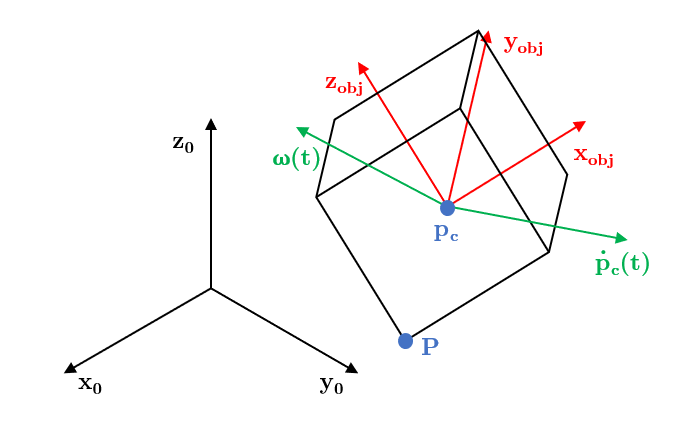
\includegraphics[width=0.7\columnwidth]{Imagens/CorpoRig.PNG}
\caption{Corpo rígido com vetores de velocidade linear e angular.}
\label{fig:CorpoRig}
\end{figure}

Derivando a Equação \ref{eq:3_16} ao longo do tempo, pode-se obter a relação dada pela Equação \ref{eq:3_17}. Utilizando da propriedade apresentada na Equação \ref{eq:3_13}, e realizando uma relação vetorial das posições dos pontos de origem, central e da partícula, é possível obter as igualdades dadas pela Equação \ref{eq:3_18} e \ref{eq:3_19}.

\begin{equation}
\dot{p}^P_0 = \dot{Q}(t)p^P_{obj} + \dot{p}_c(t)
\label{eq:3_17}
\end{equation}

\begin{equation}
\dot{p}^P_0 = S(\omega(t))Q(t)p^P_{obj} + \dot{p}_c(t)
\label{eq:3_18}
\end{equation}

\begin{equation}
\dot{p}^P_0 = S(\omega(t))(p^P_0(t) - p_c(t)) + \dot{p}_c(t)
\label{eq:3_19}
\end{equation}

Por fim, aplicando a propriedade apresentada na Equação \ref{eq:3_18} e aplicando na Equação \ref{eq:3_19}, é possível obter um produto vetorial que pode ser observado pela Equação \ref{eq:3_20}.

\begin{equation}
\dot{p}^P_0 = \omega(t) \times (p^P_0(t) - p_c(t)) + \dot{p}_c(t)
\label{eq:3_20}
\end{equation}

Assim, pode-se observar a contribuição da velocidade angular da partícula através de $\omega(t) \times (p^P_0(t) - p_c(t))$, enquanto a contribuição da velocidade linear se dá por $\dot{p}_c(t)$. Dessa forma, é possível traçar as jacobianas de posição e orientação a fim de analisar ambas as velocidades em uma relação linear com as velocidades das configurações. Omitindo a variável $t$ para tornar o processo mais simples de compreensão, e considerando $R_x(q)$, $R_y(q)$ e $R_z(q)$ as linhas da matriz $Q$, as jacobianas podem ser representadas pelas Equações \ref{eq:3_21} e \ref{eq:3_22}.

\begin{equation}
J_p(q) = \frac{\partial p_c}{\partial q}
\label{eq:3_21}
\end{equation}

\begin{equation}
J_{\omega}(q) =
\begin{bmatrix}
R_y(q)^T \frac{\partial R_z(q)}{\partial q}\\
R_z(q)^T \frac{\partial R_x(q)}{\partial q}\\
R_x(q)^T \frac{\partial R_y(q)}{\partial q}\\
\end{bmatrix}
\label{eq:3_22}
\end{equation}

Analisando do ponto de vista do efetuador, e utilizando as relações apresentadas acima, é possível determinar as matrizes jacobianas do efetuador. Seja $n$ o \textit{frame} da última junta antes do efetuador, é possível definir as relações das Equações \ref{eq:3_23} e \ref{eq:3_24}.

\begin{equation}
J^{ef}_p(q) = -S(Q^n_0(q)p^{ef}_n)J^n_{\omega}(q) + J^n_p
\label{eq:3_23}
\end{equation}

\begin{equation}
J^{ef}_{\omega}(q) = J^n_{\omega}(q)
\label{eq:3_24}
\end{equation}

%-------------------------------------------------------------
%\susubsection{\textit{Cinemática Diferencial no efetuador}}\label{sec:Cap3_AnaEf}

% O efetuador faz parte de um extremo de um corpo rígido que possui seu outro extremo afixado em um elo. É importante compreender como as velocidades das configurações podem interferir na velocidade do efetuador. Para isso, é necessário entender a velocidade relativa em um corpo rígido. Com referência a Figura \ref{fig:DoisPontos}, considerando a transformação do \textit{frame} de coordenada centrada no ponto $P_0$ para o de $P_1$, pode-se obter a seguinte relação:


 
%-------------------------------------------------------------
\subsection{\textit{Controle Cinemático}}\label{sec:Cap3_ControleCin}

Na área da robótica, evita-se realizar o controle direto do torque dos manipuladores a fim de evitar possíveis danos nos equipamentos e a terceiros. Nesse sentido, controla-se a posição através da função tarefa, que se trata de uma função que determina a realização de uma tarefa do manipulador – como alcançar a pose do efetuador desejada –, através das configurações das juntas, ao longo do tempo. Há diversas formas de se projetar a função tarefa, porém ela precisa ser diferenciável em $q$ e em $t$.

Uma tarefa é finalizada se, e somente se, $r(q,t) = 0$. Uma estratégia utilizada para verificar se a posição do objeto foi alcançada, é realizando a subtração dos pontos espaciais entre o ponto de posição desejada e a posição atual. Já para a tarefa de orientação, é realizado o produto escalar entre as componentes cartesianas – $x$, $y$ e $z$ – da orientação desejada e da atual. Para isso, as componentes necessitam ter normas unitárias, e verifica-se a seguinte relação encontrada na Equação \ref{eq:3_25}, juntamente com a tarefa de posição, a qual $r(q,t) = 0$ se, e somente se, elas coincidirem.

\begin{equation}
r(q,t) = 
\begin{bmatrix}
p(q)-p_{des}(t)\\
1-\hat{x}(q)^T\hat{x}_{des}(t)\\
1-\hat{y}(q)^T\hat{y}_{des}(t)\\
1-\hat{z}(q)^T\hat{z}_{des}(t)\\
\end{bmatrix}
\label{eq:3_25}
\end{equation} 

% O mesmo pode se realizado para a orientação, sendo este utilizando a mesma estratégia adotada na Equação \ref{eq:3_25}, porém utilizando os eixos para verificar o alinhamento com o desejado.

Definida a função tarefa, é possível implementar a ação de controle. Derivando a função tarefa no tempo, é possível encontrar, através de equações diferenciais e regra da cadeia, a seguinte relação descrita na Equação \ref{eq:3_26}.

\begin{equation}
\frac{dr(q,t)}{dt} = \frac{\partial r(q)}{\partial q} \frac{dq(t)}{dt} + \frac{\partial r(q,t)}{\partial t}= J_r(q) \dot{q} + \frac{\partial r(q,t)}{\partial t}
\label{eq:3_26}
\end{equation}

A Equação \ref{eq:3_26} também pode ser descrita da seguinte forma:

\begin{equation}
\frac{\partial r(q)}{\partial q} \dot{q} = -Kr(q(t)) - \frac{\partial r(q,t)}{\partial t}
\label{eq:3_27}
\end{equation}

\begin{figure}[b!]
\centering
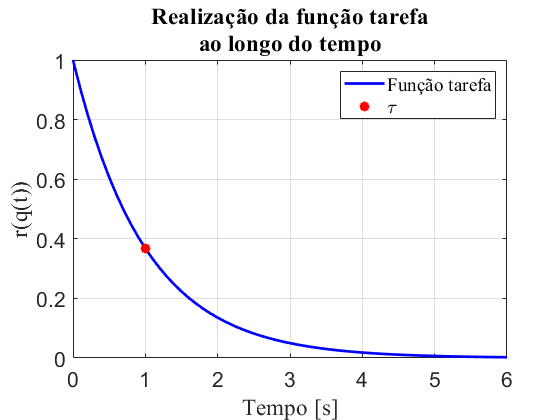
\includegraphics[width=0.7\columnwidth]{Imagens/FuncaoTarefa.png}
\caption{Gráfico da função tarefa ao longo do tempo.}
\label{fig:FuncaoTarefa}
\end{figure}

A parcela $\dot{q}$ representa a ação de controle $u(q)$, que permite uma convergência exponencial da tarefa. Já $K$, é uma constante que está relacionada a velocidade em que a tarefa é executada, sendo $\tau$ a constante de tempo que compreende a 62,83\% da execução, e $\tau = \frac{1}{K}$ como pode ser observado na Figura \ref{fig:FuncaoTarefa}. Por fim, a parcela de $\frac{\partial r(q,t)}{\partial t}$ representa um termo de \textit{feedfoward}, que permite que a resposta da saída acompanhe a entrada de referência variante no tempo. Assim, assumindo que $J_r(q)$ é invertível, pode-se obter que a ação de controle conforme descrito na Equação \ref{eq:3_28}.

\begin{equation}
u(q) = J_r(q)^{-1} (-Kr(q(t)) - \frac{\partial r(q,t)}{\partial t})
\label{eq:3_28}
\end{equation}

% \begin{figure}[b!]
% \centering
% 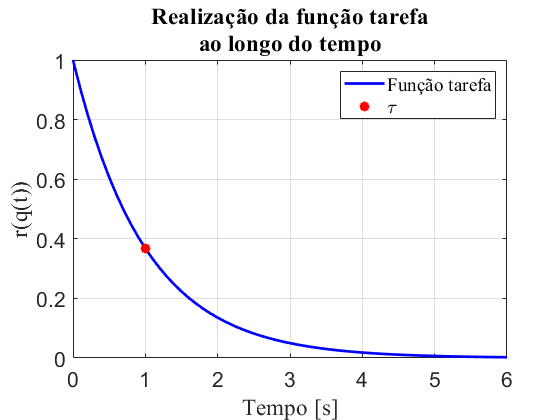
\includegraphics[width=0.7\columnwidth]{Imagens/FuncaoTarefa.png}
% \caption{Corpo rígido com vetores de velocidade linear e angular.}
% \label{fig:FuncaoTarefa}
% \end{figure}

Apesar disso, nem sempre é possível inverter a Jacobiana de tarefa, uma vez que a Equação \ref{eq:3_27} pode ser um problema de nenhuma ou infinitas soluções. Nesse caso, o objetivo é obter um valor mais próximo do esperado e que exija um menor esforço computacional. Assim, a fim de obter uma solução de otimização, e omitindo a variável $q$ e $t$ para tornar o processo mais simples de compreensão, é utilizada a pseudoinversa da matriz da Jacobiana de tarefa, definida na Equação \ref{eq:3_29}\footnote{Uma matriz pseudo inversa é originalmente representada por $J_r^+$, porém, por motivos de desambiguação, foi optado por representar neste projeto por $J_r^{\dagger}$.}, a qual substituindo-a na Equação \ref{eq:3_28}, obtém-se a relação da Equação \ref{eq:3_30}.

\begin{equation}
J_r^{\dagger} = (J_r^T J_r + \epsilon I_{n\times n})^{-1} J_r^T
\label{eq:3_29}
\end{equation}

\begin{equation}
u = J_r^{\dagger} (-Kr - \frac{\partial r}{\partial t})
\label{eq:3_30}
\end{equation}

É importante ressaltar que, na Equação \ref{eq:3_29}, tem-se $\epsilon \rightarrow 0^+$, e que o valor da ação de controle pode se tornar muito instável e ruidoso. Para corrigir isso e evitar um esforço computacional excedente, é utilizado a pseudoinverda amortecida, a qual $\epsilon$ assume um valor baixo, mas que não tende a um valor nulo. Nessa nova expressão, a pseudoinversa amortecida pode ser descrita da seguinte forma:

\begin{equation}
J_r^{\dagger (\epsilon)} = \frac{J_r}{J_r^2 + \epsilon}
\label{eq:3_31}
\end{equation}

A qual o maior valor possível é $J_r^{\dagger (\epsilon)} = \frac{1}{2 \sqrt{\epsilon}}$. Assim, quanto maior o valor de $\epsilon$, menor a variação da ação de controle, porém que pode ser mais distante da solução ideal. Assim, a estratégia de controle pode ser definida pela Equação \ref{eq:3_32}.

\begin{equation}
u = J_r^{\dagger (\epsilon)} (-Kr - \frac{\partial r}{\partial t})
\label{eq:3_32}
\end{equation}

Com base nas Jacobianas de posição e orientação fornecidas pelas Equações \ref{eq:3_23} e \ref{eq:3_24}, é possível encontrar a Jacobiana de tarefa do efetuador através da Equação \ref{eq:3_33}.

\begin{equation}
J_r(q,t) =
\begin{bmatrix}
J_p(q)\\
x_{des}^T S(x_{ef}(q)) J_{\omega}(q)\\
y_{des}^T S(y_{ef}(q)) J_{\omega}(q)\\
z_{des}^T S(z_{ef}(q)) J_{\omega}(q)\\
\end{bmatrix}
\label{eq:3_33}
\end{equation}

% \begin{figure}[h!]
% \centering
% 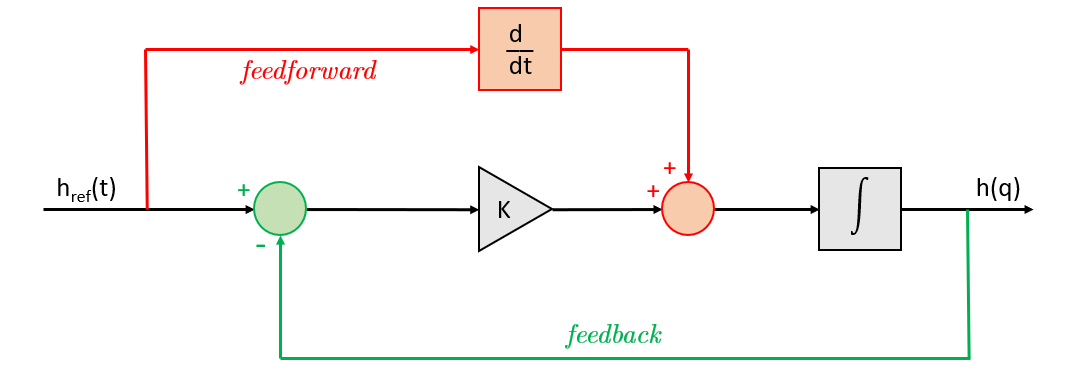
\includegraphics[width=0.7\columnwidth]{Imagens/DiagramaBlocos.PNG}
% \caption{Diagrama de blocos de controle do manipulador.}
% \label{fig:DiagramaBlocos}
% \end{figure}

Por fim, é possível obter o diagrama de blocos de controle do manipulador, disponível na Figura \ref{fig:DiagramaBlocos}, a fim de compreender o funcionamento do projeto. A função tarefa desse diagrama é detalhada na Equação \ref{eq:3_34}.

\begin{equation}
r(q,t) = h(q) - h_{ref}(t)
\label{eq:3_34}
\end{equation}

\begin{figure}[h!]
\centering
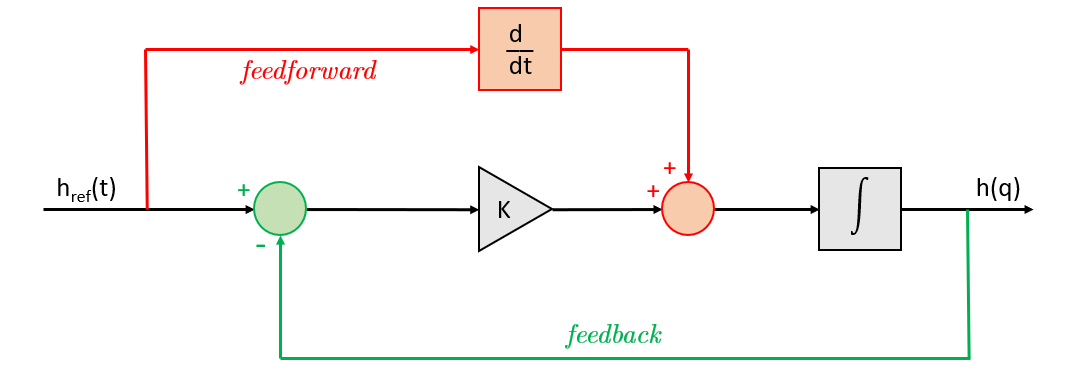
\includegraphics[width=0.7\columnwidth]{Imagens/DiagramaBlocos.PNG}
\caption{Diagrama de blocos de controle do manipulador.}
\label{fig:DiagramaBlocos}
\end{figure}

%===========================================================
\section{\textit{Simulação do Sistema e Prototipação}}\label{sec:Cap3_Simulador}

O manipulador é composto por eixos e juntas, a qual possuem representação espacial como demonstrado na seção \ref{sec:Cap3_Espacial}. A plataforma CoppeliaSim, antes chamada de V-REP, possui modelos de manipuladores capazes de representar suas limitações e ações possíveis. Ela é amplamente utilizada na área de robótica e possui uma versão educacional que oferece total capacidade de simulação e de edição.

A plataforma possui suporte a integração com o MATLAB, além de possuir bibliotecas prontas para linguagem Python. O MATLAB, por sua vez, é uma plataforma que consegue lidar bem com processamento de dados que envolvam matrizes, processamento de sinais, análise númerica e construção de gráficos. Ele possui um pacote de suporte ao uso de Arduino, um microcontrolador de baixo custo recomendado na construção de protótipos.

Como já foi abordado na seção \ref{sec:Cap3_Deteccao}, existem muitas bibliotecas criadas para a linguagem Python para detecção de objetos. Dessa forma, é possível integrar as bibliotecas utilizadas em um mesmo ambiente, a fim de reduzir o número de plataformas e ambientes de desenvolvimento integrado (IDE) utilizados. Um editor de código-fonte que tem crescido bastante e ganhado suporte da comunidade desenvolvedora através de extensões, é o  Visual Studio Code (VSCode), criado pela Microsoft. Ele é aberto e gratuito, além de possuir suporte para depuração, controle de versão, entre muitos outros recursos. Ele foi escolhido pela facilidade do uso de suas extensões distribuídas pela comunidade, além de exigir menos esforço em sua execução frente a IDEs que recorrem de mesmas funções utilizadas para este projeto.

Assim, é possível projetar os ambientes para a execução de cada etapa para os objetivos de simular e realizar a validação através de um protótipo. Para a simulação, foi planejado utilizar elementos do CoppeliaSim para simular um enquadramento da imagem de uma câmera. Dessa forma, todo o tratamento deste enquadramento é realizado no VSCode, e os dados do melhor posicionamento são enviados para o MATLAB. Assim, a estrutura de controle é tratada e enviada para realização da simulação do manipulador robótico no CoppeliaSim. Esse processo se repete, de forma a sempre conseguir o posicionamento mais adequado no efetuador do manipulador – onde se encontra a câmera. As etapas podem ser observadas na Figura \ref{fig:DiagramaSimulacao}.

% \begin{figure}[h!]
% \centering
% 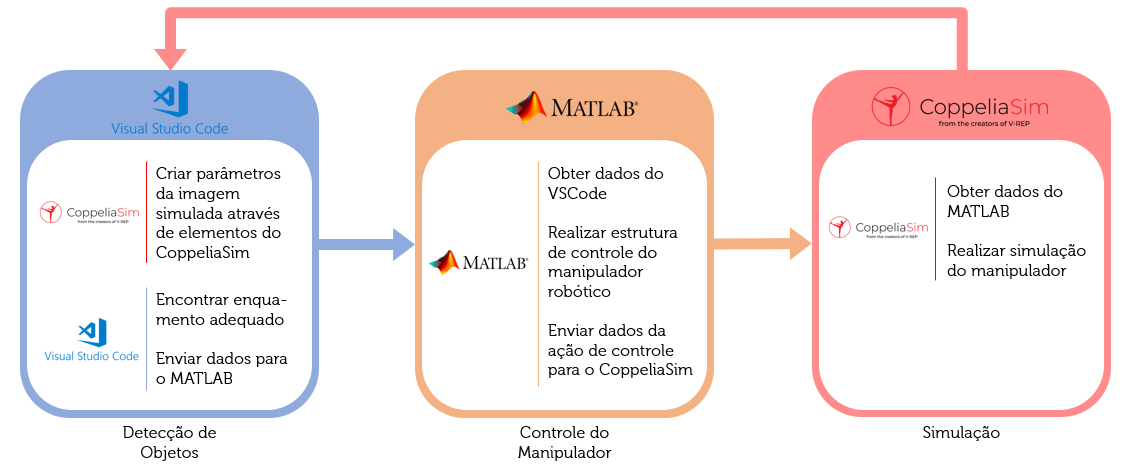
\includegraphics[width=0.9\columnwidth]{Imagens/DiagramaSimulacao.PNG}
% \caption{Diagrama de etapas para simulação do projeto.}
% \label{fig:DiagramaSimulacao}
% \end{figure}

Para a execução do protótipo, muitas etapas são semelhantes a simulação. Primeiro, as imagens da câmera são obtidas através da biblioteca OpenCV, e é realizada a detecção de pessoas nas imagens e suas posições no enquadramento através do TensorFlow. Logo, é obtido o melhor posicionamento dentro do enquadramento de imagem, e esses dados são enviados para o MATLAB, a qual será responsável por toda parte de controle do manipulador robótico. Este, por sua vez, envia os dados da ação de controle para o Arduino, que é responsável pela ativação dos motores para movimentação do manipulador. Esse processo se repete, de forma a sempre conseguir o posicionamento mais adequado no protótipo – que serve de suporte para a câmera. As etapas podem ser observadas na Figura \ref{fig:DiagramaPrototipo}.

\begin{figure}[h!]
\centering
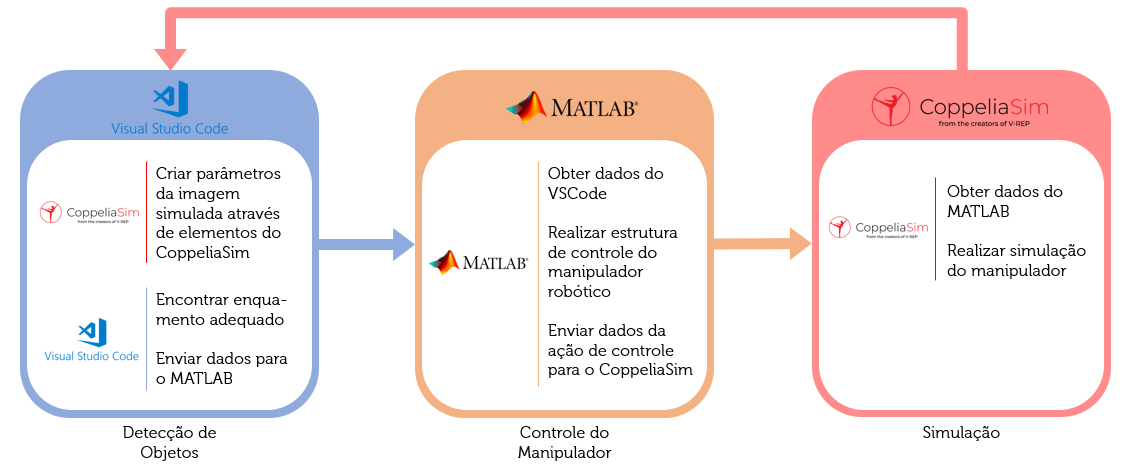
\includegraphics[width=0.9\columnwidth]{Imagens/DiagramaSimulacao.PNG}
\caption{Diagrama de etapas para simulação do projeto.}
\label{fig:DiagramaSimulacao}
\end{figure}

\begin{figure}[h!]
\centering
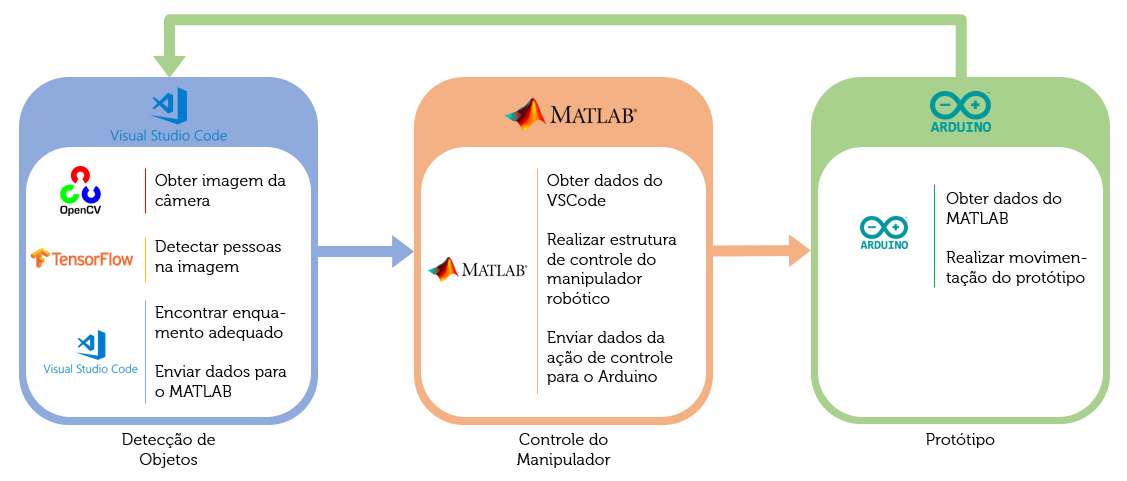
\includegraphics[width=0.9\columnwidth]{Imagens/DiagramaPrototipo.PNG}
\caption{Diagrama de etapas para execução do protótipo.}
\label{fig:DiagramaPrototipo}
\end{figure}



\textcolor{white}{.}



\chapter{Cronograma}
\label{sec:metodologia}


\begin{table}[!h]
    \centering
    \begin{tabular}{c|c}
        Data limite estimada & Atividade \\
        \hline
         15/12/2021 & Finalização do script para simulação do projeto\\
         22/12/2021 & Finalização do script para prototipação do projeto\\
         20/01/2022 & Montagem e teste do protótipo\\
         02/02/2022 & Finalização da monografia\\
         10/02/2022 & Finalização da apresentação do TCC\\
    \end{tabular}
    \caption{Cronograma de desenvolvimento do Trabalho de Conclusão do Curso}
    \label{tabt3:params}
\end{table} 

% \textual
% % ----------------------------------------------------------
% Introdução (exemplo de capítulo sem numeração, mas presente no Sumário)
% ----------------------------------------------------------
\chapter[Introdução]{Introdução}
%$\addcontentsline{toc}{chapter}{Introdução}
% ----------------------------------------------------------    

Human: How many countries are there?

VANT ou veiculos autonomos aéreos não tripulados possuem crescente potencial e  aplicação nas indústrias agricolas,
militares e serviços. E para que sua navegação seja realizável, é imprescindível a implementação de um sistema de
localização robusto [citar business report]. As formas de localização mais amplamente utilizadas são a partir de GPS
podendo ser combinados ou não com fusão sensorial à uma IMU \-- Unidade de medição inercial. O GPS embora tenha
acurácia da ordem de poucos metros, possui o compromisso de ter baixa taixa de amostragem. Isso pode ser mitigado com a
fusão
sensorial com medições da IMU, assim obtendo melhores estimativas de posição. A estimação de posição utilizando somente
a IMU também pode não ser adequada pelo fato da estimativa ser calculada integrando as medições de aceleração e assim
possuindo alto drift. Dessa forma,
essa estimação clássica de posição é mais adequada pelo conjunto de ambos.
Este conjunto, contudo, deixa de ser preciso quando não há a disponibilidade de GPS. Essas condição pode ocorrer por
eventuais indisponibilidades, também por interferencias destrutivasm comuns em um ambiente urbando ou por signal jamming
deliberadamente. Ambientes urbanos possuem superfícies metálicas que refletem o sinal transmitido pelos satélite. Tal
sinal refletido ao chegar no receptor GPS pode gerar interferências destrutivas com o sinal original desejado. Signal
jamming é uma vulnerabilidade comum para drones, seja de aplicações civis ou militares, já que um agente maliciosoo pode
desabilitar a localização ou comunicação do drone por meio de um sinal de interferência. 

Para que a localização seja realizada, é necessário que o drone possua um sistema de localização robusto. E neste
trabalho será proposto e implementado um sistema de localização via pattern matching complementar as localizações
anteriormente citadas. O patern matching será feito a partir da comparação das imagens de georeferendiadas de satélite
com as imagens captturadas instantaneamente. Além disso, terá como escopo portar o modelo de reconhecimento de padrões
para o hardware limitado do drone e metodologias de reduzir o custo computacional de avaliação de padrões.


Todo trabalho será desenvolvido com apoio do laboratório MINDS (Machine Intelligence and Data Science) da Universidade Federal de Minas
Gerais interno a Escola de Engenharia, que possui o ferramental e orientação.


Receptores ópticos têm uma vasta gama de aplicações. Podemos utilizá-los para detectar a presença ou ausência de luz no
ambiente em determinada faixa de frequência; recepção de sinais luminosos de diferentes cores para criar uma foto;
recepção de sinais codificados em luz para realizar uma transmissão de dados sem fio (Li-Fi); detecção de temperatura em
um objeto via a sua emissão de luz infravermelha; entre incontáveis outras utilidades. A forma como o circuito do sensor
é desenvolvido varia muito com a aplicação, e diversas topologias podem ser utilizadas. Mesmo dentro de uma classe
específica de sensores, diversas variações de circuitos podem existir.

Neste trabalho, é desenvolvido o projeto eletrônico dos principais blocos analógicos de um Receptor \'Optico integrado
em tecnologia CMOS de 180 nm. Para realizar a recepção dos dados, um pixel ativo do tipo APS (\textit{Active Pixel
Sensor}) e um TIA (\textit{Transimpedance Amplifier}) para captação de refer\^encia de temporização foram projetados. O
APS e o TIA são topologias muito estudadas e utilizadas, devido principalmente à facilidade com que podem ser integrados
em um CI utilizando tecnologia CMOS e também sua facilidade de acoplamento com outros circuitos do mesmo CI. 

Junto à construção dos blocos citados, diversos outros circuitos são necessários para que se permita o condicionamento e
processamento do sinal luminoso transferido para o domínio elétrico. Dentre os circuitos auxiliares que compõem todo um
sistema de Pixel Ativo, podemos citar Amplificadores Operacionais, utilizados para amplificar o sinal gerado pelo
sensor; circuitos geradores de temporização, que definem o momento de captação de luz do pixel, e o momento este poderá
ser operado; e circuitos de controle que devem ser utilizados para garantir sincronia entre todos elementos do sistema

O desenvolvimento dos principais circuitos analógicos de um Receptor Óptico integrado serão apresentados, desde o seu
detalhamento teórico, concepção do circuito e subcircuitos necessários ao sistema, desenvolvimento de esquemático para
realização de simulações iniciais, construção do layout de circuito integrado, desenvolvimento de um CI para permitir a
ligação dos sinais e realização de testes, e finalmente, simulações para validação de todo sistema. A tecnologia
utilizada no processo é a \textit{CMOS TSMC 180nm}.

Todo o trabalho é desenvolvido com apoio do OptMA\textsuperscript{Lab} , laboratório que se apresenta internamente à
Escola de Engenharia da UFMG, e que possui o ferramental necessário para permitir a realização de todos o procedimentos
aqui citados, com exceção da fabricação do APS e seu encapsulamento, que é realizada em local externo por meio de uma
parceria da universidade com a IMEC (\textit{Interuniversity Microelectronics Centre}).

\section{Motivação e Objetivos do Trabalho}

Dado a infinidade de aplicações do qual um APS pode ser utilizado, a fundamentação de parâmetros de referência para
desenvolvimento de projetos de circuitos que se faz presente é de essencial importância para possibilitar a escolha de
qual projeto é mais adequado à aplicação. Diferentes figuras de mérito podem ser avaliadas para otimizar uma ou mais
características de interesse técnico e/ou econômico do projeto.

O trabalho tem como principal objetivo o desenvolvimento de um circuito de Sensor de Pixel Ativo, e um TIA, tomando como
referência trabalhos j\'a desenvolvidos por outros autores. O desenvolvimento apresenta o projeto elétrico, simulação, e
desenvolvimento do layout do CI (\textit{Circuito Integrado}). 

São desenvolvidos seis circuitos principais, sendo três com a função de detectar diferentes cores (azul, verde e
amarelo) utilizando um APS, um circuito extrator de sinal de relógio de uma fonte luminosa atrav\'es de um TIA, e um APS
e um TIA para fins de testes, dos quais são utilizados para testar as funcionalidades dos circuitos citados sem a
necessidade de uma fonte luminosa. 

O dispositivo projetado deve se adequar a todas as características recomendáveis de um projeto de circuito analógico
integrado CMOS, devendo ser avaliado e otimizado para aprimorar certas propriedades importantes de layout como perdas
ohmicas, capacitâncias parasitas, ruídos e consumo.

Alguns circuitos auxiliares compõem conjuntamente o projeto, como Amplificadores Operacionais, Filtros e
Multiplexadores, que são elementos comuns em projetos de APS’s e TIA's, utilizados para transferir e controlar a
informação gerada pelo sensor, mas que não são o principal foco de análise.

\section{Estrutura do Trabalho}

A monografia apresenta o desenvolvimento de um projeto de Receptores Ópticos. O texto foi dividido em quatro capítulos,
além desta introdução, sendo eles Revisão Bibliográfica, Desenvolvimento do Projeto, Resultados e Conclusão.

Revisão Bibliográfica, capítulo 2 deste trabalho, visa apresentar um resumo histórico simplificado sobre Receptores
Ópticos, conceituação de elementos chave para o entendimento do que é apresentado em capítulos posteriores, citação de
outros trabalhos relacionados ao tema aprovados pela comunidade científica e detalhamento dos circuitos APS e TIA,
principais objetos de estudo deste documento.

Desenvolvimento do Projeto, capítulo 3 deste trabalho, visa apresentar o processo adotado para desenvolvimento do
Receptor Óptico, as especificações e tecnologias utilizadas pelo autor, e mostrar o esquemático elétrico dos blocos de
maior interesse para entendimento do projeto. O desenvolvimento a nível de layout do circuito também é apresentado, com
base nos circuitos previamente indicados.

Resultados, capítulo 4 deste trabalho, apresenta todos resultados de simulação obtidos de acordo com o modelo metodológico previamente apresentado, e a comprovação de atendimento aos objetivos tais quais formulados.

Conclusão, capítulo 5 deste trabalho, retoma os resultados e avalia se os objetivos foram devidamente alcançados. Sugestões de trabalhos posteriores são apresentados para explorar alguns tópicos que o autor entende que possam complementar todo o estudo aqui realizado.

\section{Padronização de identifição dos elementos dos circuitos}
\label{section:padrao_sinais}

Para facilitar a demonstração dos circuitos presentes neste trabalho, o autor padronizou um conjunto de cores que estarão presentes em cada elemento ilustrado para cada circuito referenciado:

\begin{itemize}
    \item \textbf{\color{red}VERMELHO}: indica o nome de uma inst\^ancia de um componente
    \item \textbf{\color{orange}LARANJA}: indica o nome de um sinal interno
    \item \textbf{\color{green}VERDE}: indica um sinal de entrada
    \item \textbf{\color{blue}AZUL}: indica um sinal de sa\'ida
    \item \textbf{\color{gray}CINZA}: indica o nome de um sinal bidirecional (entrada e/ou sa\'ida)
\end{itemize}

% \begin{equation}
% R = 
% \begin{bmatrix}
% x'  y'  z'
% \end{bmatrix}
% = \begin{bmatrix}
% x'_x & y'_x & z'_x \\
% x'_y & y'_y & z'_y \\
% x'_z & y'_z & z'_z
% \end{bmatrix}
% = \begin{bmatrix}
% x'_x & y'_x & z'_x \\
% x'_y & y'_y & z'_y \\
% x'_z & y'_z & z'_z
% \end{bmatrix} 
% \label{eq:3_04}
% \end{equation}\\
% % ----------------------------------------------------------
% Introdução (exemplo de capítulo sem numeração, mas presente no Sumário)
% ----------------------------------------------------------
\chapter[Revisão Bibliográfica]{Revisão Bibliográfica}
%$\addcontentsline{toc}{chapter}{Introdução}
% ----------------------------------------------------------

A literatura sobre Receptores Ópticos \'e extensa e contempla os mais diversos aspectos sobre o tema, desde o entendimento do fenômeno físico, diferentes topologias e estrat\'egias para otimização de diferentes características do circuito, circuitos auxiliares necessários para a transferência de informação, e tamb\'em o layout do projeto. Este capítulo tem como objetivo contextualizar e fundamentar algumas discussões de capítulos posteriores, demonstrar alguns trabalhos previamente realizados na área, e dar uma perspectiva histórica sobre algumas tecnologias envolvidas.
\section{Histórico}
O interesse de extrair informações advindas do espectro eletromagn\'etico \'e a muito tempo de grande interesse para físicos e engenheiros. As suas aplicações são diversas, desde extrair cores para formar uma imagem at\'e extrair informação digital de acordo com um sinal luminoso modulado.
Em 1949, a primeira patente relacionada a um dispositivo semicondutor capaz de transformar informações luminosas em el\'etricas foi requisitada pela Bell Labs, sendo oficialmente aceita em 1951. Era o nascimento do fototransistor, um transistor bipolar especial que capta informação luminosa em sua base, gerando uma informação por forma de uma corrente el\'etrica em seu coletor e emissor \cite{Shive}.

Com a invenção do fototransistor e fotodiodo, e o desenvolvimento de tecnologias de fabricação de semicondutores, se gerou uma intensa pesquisa na d\'ecada de 60, que culminou no desenvolvimento do CCD (\textit{Charge Coupled Device}) no início da d\'ecada de 70, sendo a tecnologia de Recepção Óptica mais utilizada at\'e a d\'ecada de 90 \cite{EstevaoCoelho, Andre}.

Em meados da d\'ecada de 70, o PPS (\textit{Passive Pixel Sensor}) foi desenvolvido, como alternativa aos dispositivos de imagem de tubo a vácuo \cite{Savvas}. Sua constituição se dá por uma matriz de fotodiodos, que convertem uma informação luminosa em el\'etrica, diretamente a um elemento processador de dados analógico, sem a utilização de um componente de amplificação.

Ainda na d\'ecada de 70, os primeiros trabalhos relacionados ao APS foram desenvolvidos utilizando a tecnologia MOS (\textit{Metal-Oxide-Semiconductor}) \cite{Peter}. O APS \'e uma evolução direta do PPS, com a adição de circuitos eletrônicos de condicionamento de sinal, utilizando-se amplificadores operacionais \cite{EstevaoCoelho}. Amplificar o sinal permite uma maior precisão na aquisição dos dados, al\'em de permitir uma maior miniaturização do fotodiodo, o que leva a uma miniaturização de todo o sistema. Com a evolução da tecnologia CMOS (\textit{Complementary Metal-Oxide-Semiconductor}) na d\'ecada de 90, o APS se tornou mais atraente, por ser facilmente integrado com outros componentes que utilizam-se da mesma tecnologia em um mesmo circuito integrado.

Amplificadores Operacionais são circuitos amplamente utilizados para o desenvolvimento de sistemas analógicos. Desde a década de 60, o desenvolvimento de circuitos de comunicação óptica exploram a utilização de amplificadores para captação de sinais ópticos, transmissão e regeneração de sinais. A utilização de amplificadores operacionais junto à fotodiodos, possibilitam a conversão de sinais de luz em sinais elétricos, que pode ser processado e utilizado para fins tanto analógicos quanto digitais. O circuito comumente utilizado no processo de captação óptica de sinais digitais são variações do TIA, tendo papel fundamental para a expansão tecnológica que temos desde então. \cite{ajoy, andrefontoura}.

\section{Fotodiodo}

O fotodiodo, ou fotodetector, \'e um componente optoeletrônico semicondutor que tem a função de captar um sinal eletromagn\'etico no ambiente, e então convertê-lo para uma corrente el\'etrica, chamada de corrente fotogerada, ou fotocorrente \cite{RazaviOpt}. A faixa de frequência da onda eletromagnética que pode ser captada varia em cada projeto, mas dispositivos práticos se apresentam comumente em uma banda entre o ultravioleta e o infravermelho, o que possibilita o desenvolvimento de dispositivos dentro da faixa da luz visível \cite{LidianeCampos}.

Para o entendimento do funcionamento do fotodiodo, uma fundamentação quântica da luz deve ser utilizada, com foco principal na Teoria das Bandas e no entendimento do que são os Fótons.

\subsection{Física Quântica e Fótons}
A Física Quântica nos diz que qualquer material apresenta níveis de energia possíveis dados de forma discreta (quantizada), ou seja, qualquer objeto do universo não pode ter qualquer nível de energia, mas sim valores dados de forma discreta, e que são quantificados por meio da solução da \textit{Equação de Schrödinger} do material \cite{Sze, JohnSingleton}.


\subsubsection{Teoria das Bandas}

A Teoria das Bandas nasce da observação de que comumente uma grande quantidade de níveis de energia permitidos de um material se apresentam muito próximos entre si. Desses níveis de energia, surge-se o conceito “banda de energia”, que \'e a aproximação que dentro dessa faixa de níveis concentrados, temos uma representação contínua de níveis de energia permitidos. Um material pode apresentar uma grande quantidade de bandas, sendo que duas são de extremo interesse para o estudo de semicondutores: A Banda de condução e a Banda de valência.

A Banda de valência \'e a última da qual se considera que um el\'etron está fortemente ligada a um átomo, não podendo mover livremente ao longo do material. A Banda de condução \'e a primeira banda de níveis acima da de Valência, e nele já consideramos que um el\'etron \'e livre para se movimentar no material.

\subsubsection{Fóton}

Fóton \'e uma partícula elementar que surge como resultado da liberação de energia ocasionada pela migração de um el\'etron da Banda de condução para o de valência. Este \'e o elemento fundamental constituinte da luz, e pela dualidade onda-partícula, pode ser visto tanto do ponto de vista de uma partícula, que se movimenta no espaço e pode chocar com um material; quanto de onda movimentando no espaço, apresentando uma frequência formada pela oscilação de dois campos (El\'etrico e Magn\'etico), que \'e regida pelas \textit{Leis de Maxwell} \cite{Sze, JohnSingleton}.

\subsection{Fotodiodo}
\label{secao_fotodiodo}
Um fotodiodo \'e formado por uma junção PN, que \'e a junção de um material semicondutor dopado do tipo-P com um do tipo-N, como mostrado na \autoref{fig_fotodiodo}:

\begin{figure}[!h]
	\caption{\label{fig_fotodiodo}Exemplo de construção de uma junção PN}
	\begin{center}
	    \includegraphics[scale=0.7]{Imagens/JuncaoPN.png}
	\end{center}
	\legend{Fonte: \cite{LidianeCampos}}
\end{figure}

Quando um fóton com energia suficiente para excitar o material \'e absorvido, um par el\'etron-lacuna \'e gerado (migração de um el\'etron da banda de valência para de condução), e por difusão, os el\'etrons migram para o cátodo, formando uma fotocorrente. Ajustando-se os tamanhos das camadas P, N e também a dopagem, podemos controlar a resposta em frequência do fotodiodo e qual a energia mínima do fóton necessária para que gere a fotocorrente.

A Região de Depleção é uma região de barreira de potencial formada ao redor dos contatos da junção, que é gerada com a difusão de elétrons da camada N para P já na construção do dispositivo, ocorrendo devido a diferença de concentração de elétrons em N e lacunas (espaços com ausência de elétrons mas que podem ser ocupados pelos mesmos). No fotodiodo essa é a região de maior interesse, por ser onde há a conversão de fótons em energia elétrica que pode ser aproveitada.

Com a migração dos el\'etrons, uma diferença de potencial \'e gerada entre as camadas P e N, que pode ser aproveitada para a geração de corrente el\'etrica em um circuito el\'etrico fechado \cite{hamamatsu}.
Um fotodiodo apresenta um modelo el\'etrico equivalente ilustrado na \autoref{fig_modelofotodiodo}:

\begin{figure}[!h]
	\caption{\label{fig_modelofotodiodo}Modelo el\'etrico de um fotodiodo}
	\begin{center}
	    \includegraphics[scale=0.5]{Imagens/ModeloFotodiodo.png}
	\end{center}
	\legend{Fonte: \cite{hamamatsu}}
	\label{modeloElFotodiodo}
\end{figure}

    O modelo el\'etrico apresenta a seguinte expressão:

\begin{equation}
    \label{eq_modEletFot}
    I_o = I_L - I_D - I\rq = I_L - I_S*(\exp (\frac{qV_D}{kT})-1) - I\rq
\end{equation}

Onde:
\begin{itemize}
    \item \textit{I\textsubscript{o}} \'e a corrente de saída presente na carga [\textit{A}]
    \item \textit{V\textsubscript{o}} \'e a tensão de saída [\textit{V}]
    \item \textit{R\textsubscript{L}} \'e a carga de saída [\textit{$\Omega$}]
    \item \textit{V\textsubscript{D}} \'e a tensão presente no diodo do modelo el\'etrico equivalente [\textit{V}]
    \item $I_L$ \'e a corrente fotogerada pela fonte luminosa[\textit{A}]
    \item  \textit{I\textsubscript{D}} \'e a corrente de escuro do fotodiodo (sem a presença de luz) [\textit{A}]
    \item \textit{C\textsubscript{j}} \'e a capacit\^ancia de junção [\textit{F}]
    \item \textit{R\textsubscript{sh}} \'e a resist\^encia shunt do modelo el\'etrico equivalente [$\Omega$]
    \item \textit{I\rq} \'e a corrente shunt presente na resistência shunt do modelo el\'etrico equivalente [\textit{A}]
    \item \textit{R\textsubscript{S}} \'e a resistência em s\'erie com a carga de saída do modelo el\'etrico equivalente [$\Omega$]
    \item \textit{q} \'e a carga el\'etrica de um el\'etron [\textit{C}],
    \item \textit{k} \'e a constante de Boltzmann [\textit{J.K$^{-1}$}],
    \item \textit{T} \'e a temperatura presente no fotodiodo [\textit{K}]
\end{itemize}

O fotodiodo em uma grande faixa apresenta comportamento linear em relação a quantidade de corrente fotogerada e o número de fótons recebidos, sendo essa a faixa de principal interesse em aplicações como o APS ou o TIA. Além disso, a corrente fotogerada e a queda de tensão entre os terminais do fotodiodo também tendem a apresentar resposta linear, como mostrado na \autoref{fig_respFotodiodo}. Com o aumento ou diminuição expressiva, o circuito começa a se tornar não-linear.

Nota-se na \autoref{fig_respFotodiodo} que uma corrente e tensão negativa apresenta uma maior faixa de operação antes que ocorra a saturação do circuito. Isso ocorre pois a polarização reversa do fotodiodo aumenta a região de depleção, aprimorando a captação de fótons que podem ser convertidos em um sinal elétrico. Devido a isso o fotodiodo é comumente polarizado reversamente nas suas diversas aplicações.

\begin{figure}[!h]
	\caption{\label{fig_respFotodiodo}Resposta Tensão x Corrente para dada intensidade luminosa no fotodiodo}
	\begin{center}
	    \includegraphics[scale=0.8]{Imagens/graficoRespostaFotodiodo.png}
	\end{center}
	\legend{Fonte: \cite{hamamatsu}}
\end{figure}

\subsection{Figuras de M\'erito}
Do fotodiodo podemos extrair diversas m\'etricas (Figuras de M\'erito), que são de interesse para comparar diferentes modelos. As principais Figuras de M\'erito encontradas na literatura são descritas abaixo, apresentadas em \cite{LidianeCampos}.

\subsubsection{Eficiência Quântica}
Relação entre o número de portadores detectados nos terminais das camadas PN do fotodetector, dividido pela incidência de uma determinada quantidade de fótons no fotodetector.

\begin{equation}
    \eta = \frac{N_e}{N_p}
\end{equation}

Onde:
\begin{itemize}
    \item \textit{$\eta$} \'e Efici\^encia Qu\^antica [\textit{Adm.}]
    \item \textit{N$_e$} \'e o n\'umero de portadores que podem ser detectados nos terminais externos do fotodetector [\textit{n° portadores}]
    \item \textit{N$_p$} incid\^encia de determinada quantidade de f\'otons [\textit{n° f\'otons}]
\end{itemize}

\subsubsection{Responsividade}
Razão entre a corrente fotogerada e a potência óptica incidida no fotodiodo.

\begin{equation}
    \label{eq_responsividade}
    R_\lambda = \frac{I_{PH}}{P_{FD}}
\end{equation}

Onde:
\begin{itemize}
    \item \textit{R$_\lambda$} \'e a Responsividade [\textit{A.W$^{-1}$}]
    \item \textit{I$_{PH}$} \'e a corrente fotogerada [\textit{A}]
    \item \textit{P$_{FD}$} \'e a potência \'optica presente no fotodiodo [\textit{W}]
\end{itemize}

A Eficiência Quântica e a Responsividade se relacionam de acordo com a \autoref{eqEfResp}.

\begin{equation}
    \label{eqEfResp}
    R_\lambda = \frac{\lambda\eta}{1,24}
\end{equation}

Onde:
\begin{itemize}
    \item \textit{R$_\lambda$} \'e a Responsividade [\textit{A.W$^{-1}$}]
    \item $\lambda$ \'e o comprimento de onda da luz incidente [\textit{m}]
    \item $\eta$ \'e Efici\^encia Qu\^antica [\textit{Adm.}]
\end{itemize}

A \autoref{fig_eqEfResp} mostra o gráfico da Responsividade e Efici\^encia Qu\^antica de alguns materiais.

\begin{figure}[!h]
	\caption{\label{fig_responsividade}Responsividade e Efici\^encia Qu\^antica dos materiais Ge, InGaAs, Si}
	\begin{center}
	    \includegraphics[scale=0.5]{Imagens/GraficoRespostaEspectral.png}
	\end{center}
	\legend{Fonte: \cite{ajoy}}
	\label{fig_eqEfResp}
\end{figure}


\subsubsection{Velocidade de Resposta}
A velocidade de resposta indica o quão rápido o fotodiodo \'e capaz de responder a estímulos de luz externos, em determinada frequência. É caracterizado pelo Tempo de Subida e Tempo de Descida do Fotodiodo, na faixa de frequências de interesse.

O Tempo de Subida \'e calculado como o tempo do qual um fotodiodo, inicialmente sem incidência de luz, leva para elevar o seu nível de tensão nos seus terminais de 10\% para 90\% do seu pico, a partir do no momento que começar a absorver fótons de uma fonte luminosa controlada, em determinada frequência.

O Tempo de Descida \'e calculado como o tempo do qual um fotodiodo, inicialmente com determinada incidência de luz e já estabilizado na sua respectiva tensão de pico, leva para diminuir a diferença de tensão entre seus terminais de 90\% para 10\% do seu pico, a partir do momento que não absorve mais fótons de origem de uma fonte luminosa controlada, em determinada frequência.

\begin{figure}[!h]
	\caption{\label{fig_velocidadeResp}Representação gr\'afica do Tempo de Subida e Descida}
	\begin{center}
	    \includegraphics[scale=0.3]{Imagens/GraficoVelocidadeResposta.png}
	\end{center}
	\legend{Fonte: Produzido pelo autor}
\end{figure}

O conhecimento da velocidade de resposta \'e crucial para determinar as limitações do projeto em termos de processamento de informações. A amostragem de dados deve ter período maior do que os tempos de subida e de descida do fotodiodo, nos maiores valores apresentados na faixa de frequência desejada.

\subsubsection{Resposta Espectral}

O Efeito Fotoel\'etrico se caracteriza pela excitação de el\'etrons em um material por um fóton, quando este apresenta uma energia mínima, chamada de \textit{Função Trabalho}. Mesmo quando uma grande quantidade de fótons com energia menor do que a Função Trabalho atravessem o fotodiodo, eles não serão capazes de excitar nenhum el\'etron. Como a energia de um fóton diminui com o aumento de seu comprimento de onda, existe um comprimento de onda máximo (ou uma frequência mínima) do qual o fotodetector será capaz de gerar fotocorrente.

Por outro lado, uma diminuição do comprimento de onda tende a excitar cada vez menos el\'etrons, pois absorção de luz acontece principalmente na superfície da região de difusão, que não é a região de depleção.

Sabendo destas limitações, definimos a Resposta Espectral como a faixa de comprimentos de onda do qual o fotodetector \'e capaz de produzir uma fotocorrente correspondente.

\section{Sensor de Pixel Ativo (APS)}
\label{section:APS}
Um APS \'e um dispositivo do qual se aproveita das características de um fotodiodo para gerar um sinal que pode ser amostrado e então quantificado, de forma a produzir informações referentes à luz incidida no fotodetector.

Dentre as várias possibilidades de produção de um circuito APS, aquele estudado ao longo de todo este trabalho se apresenta na \autoref{fig_APS}.

\begin{figure}[!h]
	\caption{\label{fig_APS}Circuito APS do trabalho}
	\begin{center}
	    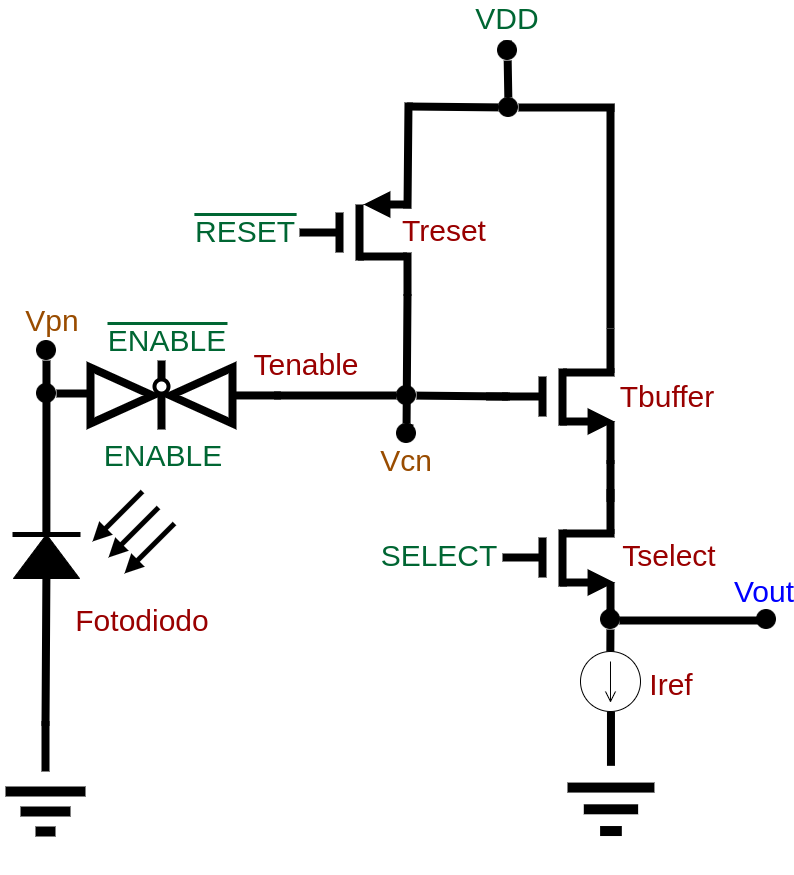
\includegraphics[scale=0.3]{Circuitos/APS.png}
	\end{center}
	\legend{Fonte: Produzido pelo autor}
\end{figure}

Cada componente desempenha uma diferente função de forma a processar a informação advinda da corrente fotogerada:

\begin{itemize}

    \item O transistor $T_{buffer}$ funciona como um amplificador de Dreno Comum, e seu papel \'e replicar o sinal advindo do n\'o central ($V_{cn}$) ao n\'o de sa\'ida ($V_{out}$), decrescido da diferença de tensão entre porta e dreno do transistor ($V_{GS}$). O efeito de carga\footnote{Efeito do qual a saída de um circuito 1, conectado a entrada de outro circuito 2, tem o valor de saída reduzido, comparado a situação da qual a saída do circuito 1 não está conectada em nada. Ocorre devido a saída do circuito 1 enxergar uma impedância finita na conexão do circuito 2, que então cria um divisor de tensão com a sua impedância de saída e consequentemente reduz a tensão vista no nó de saída.} que aconteceria caso o n\'o central fosse a saída do sistema é reduzido, pois entre os pinos de porta e dreno do transistor há a presença de uma alta impedância.

    \item O transistor $T_{reset}$ quando fechado (nível lógico '0' em seu gate) faz com que o potencial do nó $V_{cn}$ seja igual a VDD. Quando aberto (nível lógico '1' em seu gate), o sinal no n\'o central passa a depender da configuração de $T_{enable}$.

    \item A Porta de Transmissão $T_{enable}$ funciona como uma chave, e quando o transistor $T_{reset}$ estiver em aberto tem a função de isolar o fotodiodo do nó central de acordo com a sua situação de abertura ou fechamento. Quando aberto, $V_{pn}$ fica isolado do restante do circuito, devido ao estado de alta imped\^ancia nos terminais do dispositivo. Quando fechado, a corrente fotogerada descarrega em $V_{cn}$, pois a associação das capacitâncias parasitas presentes nos transistores de $T_{enable}$, $T_{reset}$ e $T_{buffer}$ formam um caminho fechado do qual descarrega lentamente o fotodiodo \cite{LidianeCampos}. Uma representação desses capacitores \'e dada na \autoref{fig_APS_cap}.
    
    \item O transistor $T_{select}$ \'e utilizado para que m\'ultiplos APS's compartilhem um mesmo barramento de sa\'ida. No projeto aqui implementado $T_{select}$ sempre se apresentar\'a fechado (\textit{SELECT} em n\'ivel l\'ogico '1').
    
    \item A fonte de corrente \textit{$I_{ref}$} tem a função de polarizar a sa\'ida do circuito, além de aprimorar a linearidade do estágio de sa\'ida \cite{RazaviFundM}.

\end{itemize}

    H\'a dois n\'os internos de bastante interesse ao trabalho, que são:

\begin{itemize}
    \item \textit{$V_{pn}$}: tensão entre os terminais do fotodiodo [\textit{V}]
    \item \textit{$V_{cn}$}: tensão no n\'o central do APS [\textit{V}]
\end{itemize}

    Os sinais externos do circuito são:
    
\begin{itemize}
    \item \textit{RESET}: fecha o transistor $T_{reset}$. Ativo em n\'ivel l\'ogico '0'.
     \item \textit{SELECT}: fecha o transistor $T_{select}$. Ativo em n\'ivel l\'ogico '1'. No circuito do trabalho estar\'a sempre configurado como '1'.
     \item \textit{ENABLE}: fecha o transmition gate $T_{enable}$. Ativo em n\'ivel l\'ogico '1'.
     \item \textit{VDD}: Alimentação do circuito
\end{itemize}

\subsection{Capacit\^ancias Parasitas}
Para o correto estudo do APS devemos observar a capacit\^ancia equivalente $C_{eq}$ presente nos n\'os $V_{pn}$ e $V_{cn}$ do circuito \cite{LidianeCampos}. Na \autoref{fig_APS_cap} temos uma representação das capacit\^ancias que compõem $C_{eq}$, que é a soma das capacitâncias apresentadas na figura.

\begin{figure}[!h]
	\caption{\label{fig_APS_cap}Representação do circuito APS com suas capacit\^ancias parasitas destacadas}
	\begin{center}
	    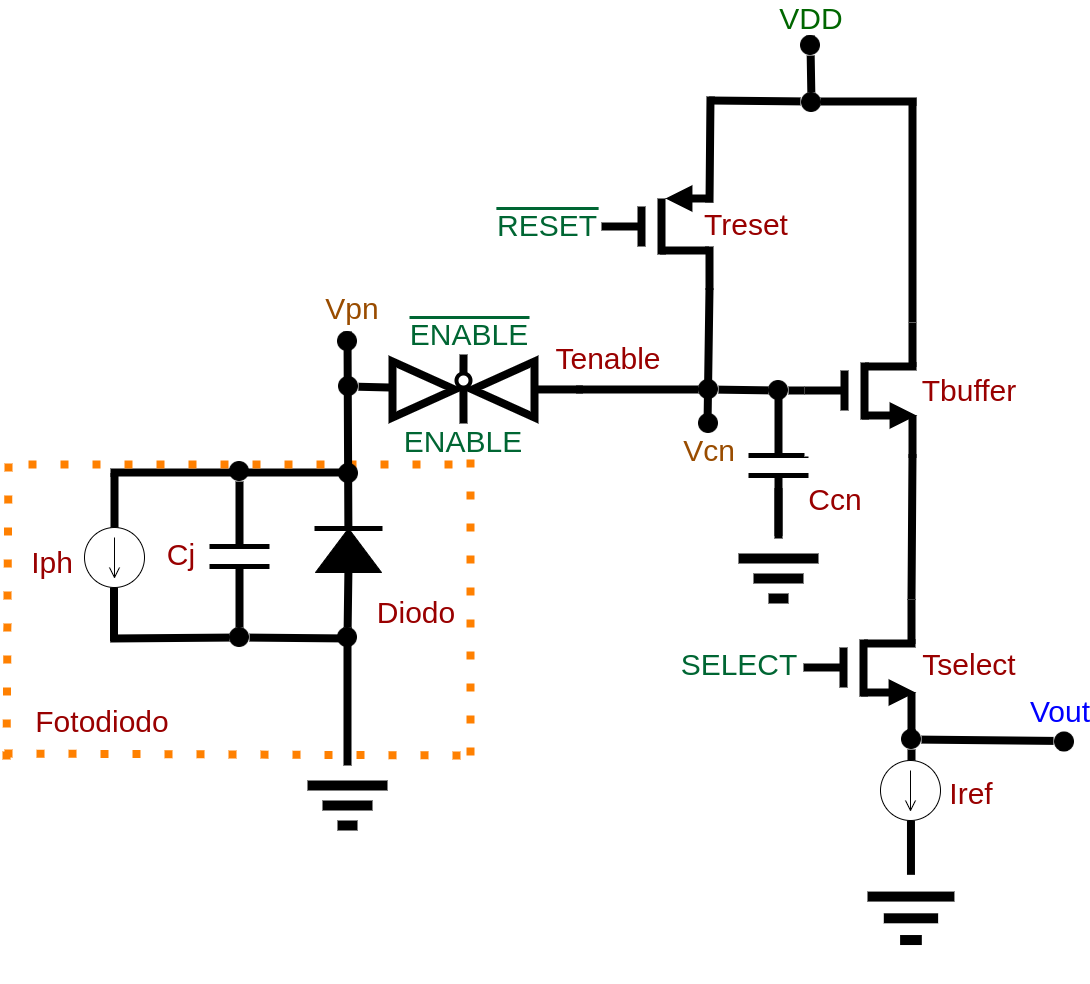
\includegraphics[scale=0.3]{Circuitos/APS_cap.png}
	\end{center}
	\legend{Fonte: Produzido pelo autor}
\end{figure}

Onde: 

\begin{itemize}
    \item $C_j$ \'e a capacit\^ancia de junção do fotodiodo. Seu principal efeito no estudo do APS \'e limitar a velocidade de variação da corrente fotogerada.
    
    \item $C_{cn}$ \'e a capacit\^ancia equivalente vista do n\'o $V_{cn}$ ao GND, devido principalmente às capacit\^ancias presentes em $T_{enable}$,  $T_{reset}$ e $T_{buffer}$, sendo o de $T_{buffer}$ o de maior contribuição. O capacitor cria um caminho fechado para a corrente do fotodiodo circular ao GND e ser descarregado em um dos est\'agios citados posteriormente no trabalho.
    
    \item $I_{ph}$ \'e a corrente fotogerada [\textit{A}].
    
    \item \textit{Diodo} \'e o diodo do modelo el\'etrico equivalente do fotodiodo.
\end{itemize}

\subsection{Est\'agios}
\label{estagiosAPS}

A operação do APS pode ser dividida em 4 est\'agios, que vão definir os m\'inimos momentos de  atuação no sinal de controle e seus limites operação. Os est\'agios são representados na \autoref{figura_estagiosAPS}, tendo como base o trabalho de \cite{LidianeCampos}.

\begin{figure}[!h]
	\caption{\label{figura_estagiosAPS}Esboço de resposta do APS ao controlar seus sinais de entrada}
	\begin{center}
	    \includegraphics[scale=0.2]{Imagens/estagiosAPS.png}
	\end{center}
	\legend{Fonte: Adaptado de \cite{LidianeCampos}}
\end{figure}

\begin{enumerate}

\item $T_{reset}$ fechado, $T_{enable}$ fechado (Período de Reset)
    
Nessa condição, o n\'o $V_{cn}$ \'e igual a VDD.

\item $T_{reset}$ aberto, $T_{enable}$ fechado (Período de Integração)

A corrente fotogerada passa a descarregar a capacit\^ancia $C_{cn}$ do nó central. A tensão no fotodiodo passa a diminuir, devido a circulação de corrente que diminui a carga de $C_{j}$.

A tensão $V_{cn}$ neste segundo est\'agio tem uma relação linear com a corrente fotogerada, conforme descrito na \autoref{eq_modEletFotIl}, que \'e deduzida fazendo an\'alises dos n\'os, desprezando-se a resistência presente em $T_{enable}$ e também outras resistências parasitas, como aquelas presentes no modelo elétrico do fotodiodo apresentado na \autoref{modeloElFotodiodo}.

\begin{equation}
    \label{eq_modEletFotIl}
    V_{cn}(t) = V_0-\frac{I_{PH}}{C_j+C_{cn}}t
\end{equation}

Onde:

\begin{itemize}
    \item $V_{cn}(t)$ \'e a tensão do nó $V_{cn}$ em determinado tempo $t$ [$V$]
    \item $V_0$ \'e a tensão do nó $V_{cn}$ no momento que o estágio inicia. Comumente deseja-se que esta tensão seja a máxima possível [$V$]
    \item $I_{PH}$ \'e a corrente fotogerada [$A$]
    \item $C_j$ \'e a capacit\^ancia de junção do fotodiodo [$F$]
    \item $C_{cn}$ \'e a capacit\^ancia do n\'o central do APS [$F$]
    \item $t$ \'e o tempo a partir do qual o estágio se iniciou [$s$]
\end{itemize}

Já a tensão de saída $V_{out}$ é dada pela \autoref{eq_voutaps}, que junto a \autoref{eq_modEletFotIl} resulta na \autoref{eq_voutfinal}, utilizada no trabalho para calcular a tensão de saída do APS em determinado instante de tempo do Estágio 2.

\begin{equation}
    \label{eq_voutaps}
    V_{out}(t) = V_{cn} - V_{GS\_buffer}
\end{equation}

\begin{equation}
    \label{eq_voutfinal}
    V_{out}(t) = V_0-\frac{I_{PH}}{C_j+C_{cn}}t - V_{GS\_buffer}
\end{equation}

Onde:

\begin{itemize}
    \item $V_{out}(t)$ \'e a tensão de saída do APS em determinado tempo $t$ [$V$]
    \item $V_{GS\_buffer}$ \'e a diferença de potencial entre $V_{cn}$ e $V_{out}(t)$, que considerando-se a ausência de efeitos de carga, e que $T_{buffer}$ esteja sempre na região de saturação no Estágio 2, é uma constante [$V$]
\end{itemize}

\item $T_{reset}$ aberto, $T_{enable}$ aberto, potencial \textit{$V_{pd}$} positivo

Logo ap\'os abrir o $T_{enable}$, a fotocorrente não circula mais no n\'o central, e o fotodiodo continua a ter sua diferença de potencial reduzida, com circulação de corrente internamente devido a $C_j$. O n\'o central passa a reduzir a tensão bem lentamente devido a correntes de fuga. \textit{$V_{pd}$} diminue seu valor at\'e se tornar negativo.

\item \textit{$T_{reset}$} aberto, \textit{$T_{enable}$} aberto, potencial \textit{$V_{pd}$} negativo

Nessa situação, o $T_{enable}$ passa a operar em modo linear. O potencial no n\'o $V_{cn}$ passa a diminuir devido a circulação de corrente do n\'o at\'e o fotodiodo. O nó diminui at\'e que finalmente chega a 0, onde se mant\'em estável e não apresenta mais circulação de corrente.

\end{enumerate}

\subsection{Amostrando informações da luz com um APS básico}
\label{secao_amostrando}

Podemos aproveitar o entendimento das propriedades f\'isicas do fotodiodo, e tamb\'em dos est\'agios de funcionamento de um APS, para obtermos informações relativas aos f\'otons absorvidos.

Como sabemos matematicamente as relações de fotocorrente determinadas por \autoref{eq_modEletFot} e \autoref{eq_modEletFotIl}, e tamb\'em as Figuras de M\'erito que caracterizam o fotodetector, podemos utilizar o APS para coletar as informações em sua sa\'ida e determinar a intensidade da luz

Entre os est\'agios 2 e 3 apresentados na \autoref{figura_estagiosAPS}, a tensão do n\'o $V_{cn}$ passa a diminuir, devido a circulação da fotocorrente. Como essa corrente depende da intensidade da luz, podemos descobrir o valor de intensidade sabendo a inclinação da curva de tensão na sa\'ida, j\'a que a variação da tensão \'e uma grandeza diretamente proporcional à corrente e a imped\^ancia vista no n\'o. Como a tensão de sa\'ida \'e igual a $V_{cn}$ menos $V_{GS}$ do transistor $T_{buffer}$, podemos medir a sa\'ida para processar o sinal e então relatar a intensidade luminosa.

Com as observações aqui apresentadas, podemos desenvolver um sistema de medição de informação luminosa, trabalhando entre os est\'agios 1 e 3, e então retornando ao Estágio 1 para uma nova aquisição. \'E importante destacar que existem limitações quanto \`a temporização dos est\'agios. Para que a medição seja realizada de forma adequada, devemos garantir que tenhamos entre o Est\'agio 1 e 2, um tempo suficientemente grande para que $V_{cn}$ apresente um valor estável, ou seja, o tempo de transição do sistema nessa condição seja conclu\'ido. Entre o Est\'agio 2 e Est\'agio 3, devemos garantir que tenhamos um tempo mínimo para que dois valores distintos de $V_{out}$ possam ser medidos, de acordo com a sensibilidade do sistema de medição.

\section{Amplificador de Transimped\^ancia (TIA)}
\label{section:TIA}

Um amplificador de transimped\^ancia \'e um circuito em que dada uma corrente de entrada, gera-se uma tensão em sua sa\'ida proporcional \`a esta corrente \cite{RazaviFundM}. Considerando-se o fotodiodo como uma fonte de corrente, a \autoref{fig_TIA} apresenta uma poss\'ivel topologia de um Amplificador de Transimped\^ancia (TIA), desenvolvido no presente trabalho.

\begin{figure}[!h]
	\caption{\label{fig_TIA}TIA desenvolvido}
	\begin{center}
	    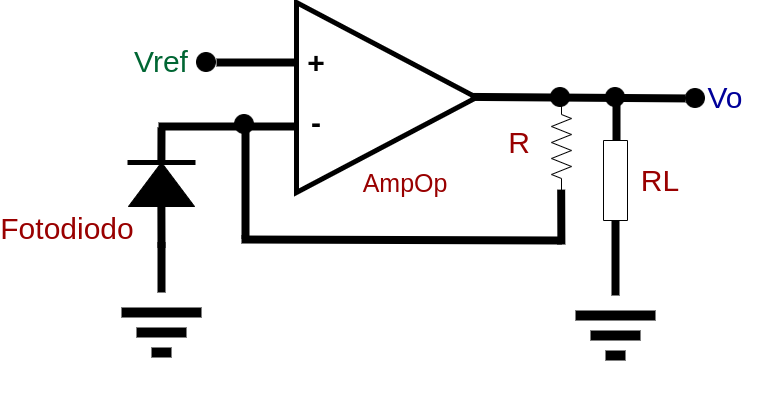
\includegraphics[scale=0.3]{Circuitos/TIA.png}
	\end{center}
	\legend{Fonte da ilustração: Pr\'oprio autor}
\end{figure}

Onde:

\begin{itemize}
    \item $V_{ref}$ \'e a tensão de entrada de referência [$V$]
    \item $V_o$ \'e a tensão de sa\'ida [$V$]
    \item $R$ \'e uma resist\^encia de ajuste ganho [$\Omega$]
    \item $R_L$ \'e uma carga de sa\'ida [$\Omega$]
\end{itemize}

Observando a \autoref{fig_modelofotodiodo}, nota-se que podemos modelar uma resist\^encia $R_{sh}$ em paralelo ao fotodiodo. Desprezando-se todos outros componentes do modelo para facilitar a an\'alise, podemos descrever a f\'ormula correspondente ao $TIA$ como a \autoref{eqCTIA}.

\begin{equation}
    \label{eqCTIA}
    V_o = RI_{PH} + (1+\frac{R}{R_{sh}})V_{ref}
\end{equation}

Onde:
\begin{itemize}
    \item $I_{PH}$ \'e a corrente fotogerada [$A$]
\end{itemize}

A \autoref{eqCTIA} nos mostra que \textit{R} deve ser ajustado de forma que não seja grande demais, pois valores altos (de acordo com a aplicação) irão gerar tensão na sa\'ida com variação muito grande. Mesmo que Vref fosse colocado em GND, o fator $(1+\frac{R}{R_{sh}})$ ainda pode dominar a relação, devido \'a ruídos presentes no nó, e então impor um termo indesejado, o que também causaria problemas quando \textit{R} fosse muito alto \cite{hamamatsu}.

Devido ao produto $RI_{PH}$, também devemos ter o cuidado de não tornar \textit{R} pequeno demais para que tenhamos a sensibilidade no sinal de saída de forma adequada.

Considerando $R_{sh} >> R$, chegamos à \autoref{eqCTIA2}, utilizada no projeto apresentado no trabalho.

\begin{equation}
    \label{eqCTIA2}
    V_o = RI_{PH}
\end{equation}

\subsection{Resposta espectral de um TIA}

Como a imped\^ancia de entrada do $TIA$ não \'e ideal (infinita) e varia com a frequ\^encia e temperatura, o circuito não se apresenta linear em toda sua banda de operação, o que representa uma variação na resposta em frequ\^encia de acordo com a corrente fotogerada \cite{hamamatsu}.
Como o pr\'oprio amplificador apresenta capacit\^ancias internas, o circuito \'e tamb\'em limitado em altas frequ\^encias, principalmente pelo produto $R$ vezes $C$, onde C \'e a capacit\^ancia interna vista pelos terminais de $R$ \cite{hamamatsu}.

A \autoref{figura_respostaTIA} e a \autoref{figura_respostaTIA2} mostram o comportamento t\'ipico de resposta em frequ\^encia da topologia. O pico observado na \autoref{figura_respostaTIA} é característico de um sistema de 2ª ordem e acontece devido a capacitância vista nos terminais do fotodiodo, em conjunto com capacitâncias internas ao amplificador e na saída. Para reduzir esse efeito, um capacitor pode ser adicionado em paralelo ao resistor \textit{R}, com valor precisamente calculado de forma a atenuar o pico (formando um circuito denominado \textit{CTIA}). A\autoref{figura_respostaTIA2} mostra as oscilações presentes em resposta a um pulso, que da mesma forma, também podem ser atenuados utilizado o mesmo capacitor.

\begin{figure}[!h]
    \begin{minipage}{0.4\textwidth}
    \centering
    \caption{\label{figura_respostaTIA}Resposta espectral de um TIA}
	\includegraphics[scale=0.8]{Imagens/RespostaEspectralTIA.png}
	\legend{Fonte: \cite{hamamatsu}}
	\end{minipage}
	 \hfill
  \begin{minipage}{0.4\textwidth}
    \centering
    \caption{\label{figura_respostaTIA2}Resposta a um pulso em um TIA}
    \includegraphics[scale=0.8]{Imagens/RespostaEspectralTIA2.png}
    \legend{Fonte: \cite{hamamatsu}}
  \end{minipage}
  
	
\end{figure}

% % ----------------------------------------------------------
% % PARTE
% % --------------------------------------------------------
% % ----------------------------------------------------------
% \chapter[Desenvolvimento do Projeto]{Desenvolvimento do Projeto}

O capítulo apresenta o projeto realizado nesta dissertação, contendo a explicação do que foi desenvolvido, os circuitos esquemáticos, os parâmetros dos componentes e os layouts dos blocos desenvolvidos. Alguns circuitos não foram incluídos neste capítulo e são apresentados de maneira implícita, devido à sua simplicidade, flexibilidade de implementação em replicações do trabalho, e devido o autor também entender que os mesmos já são de amplo conhecimento na área. No \autoref{blocosadicionais} é possível verificar mais sobre esses blocos e como foram desenvolvidos, caso o leitor sinta a necessidade de entender a sua implementação.

Ao longo de todo capítulo, tabelas serão apresentadas com as seguintes identificações

\begin{itemize}
\item $W$ é a largura do canal (transistor) ou largura do componente (resistor e diodo) [${\mu}m$]
\item $L$ é a comprimento do canal (transistor) ou comprimento do componente (resistor e diodo) [${\mu}m$]
\item $M$ é o número de dispositivos em paralelo [$n$°$ dispositivos$]
\item $S$ é o número de dispositivos em série [$n$°$ dispositivos$]
\end{itemize}

\newcommand{\NomeBloco}{NULL}
\newcommand{\NomeBlocoNoIt}{NULL}
\newcommand{\NomeBlocoNoUnderline}{NULL}
\newcommand{\NomePTab}{tab_\NomeBlocoNoUnderline}
\newcommand{\NomeSTab}{tab_\NomeBlocoNoUnderline2}
\newcommand{\NomePFig}{fig_\NomeBlocoNoUnderline}
\newcommand{\NomeSFig}{fig_\NomeBlocoNoUnderline2}
\newcommand{\NomeTTab}{tab_\NomeBlocoNoUnderline3}
\newcommand{\NomeQTab}{tab_\NomeBlocoNoUnderline4}

\section[Projeto de um Receptor Óptico]{Projeto de um Receptor Óptico}
\label{sec_circ_comp}

Um circuito integrado foi desenvolvido para a comunicação de dados via luz, utilizando-se dos circuitos apresentados na \autoref{section:APS} e \autoref{section:TIA} deste documento. O projeto \'e representado em alto n\'ivel na \autoref{fig_circcompleto}. A \autoref{fig_circcompletohigh} mostra uma representação dos principais blocos presentes no circuito.

Todos os sinais aqui apresentados na figura, e tamb\'em em todas figuras \`a seguir, seguem o padrão descrito na \autoref{section:padrao_sinais} deste trabalho.

A tensão de alimentação utilizada em todos os blocos do projeto apresentado é de \textit{1.8 V}, e é representada pelo nome \textit{VDD}.

\begin{figure}[!h]
    	\caption{\label{fig_circcompleto}Optoreceptor projetado}
	\begin{center}
	    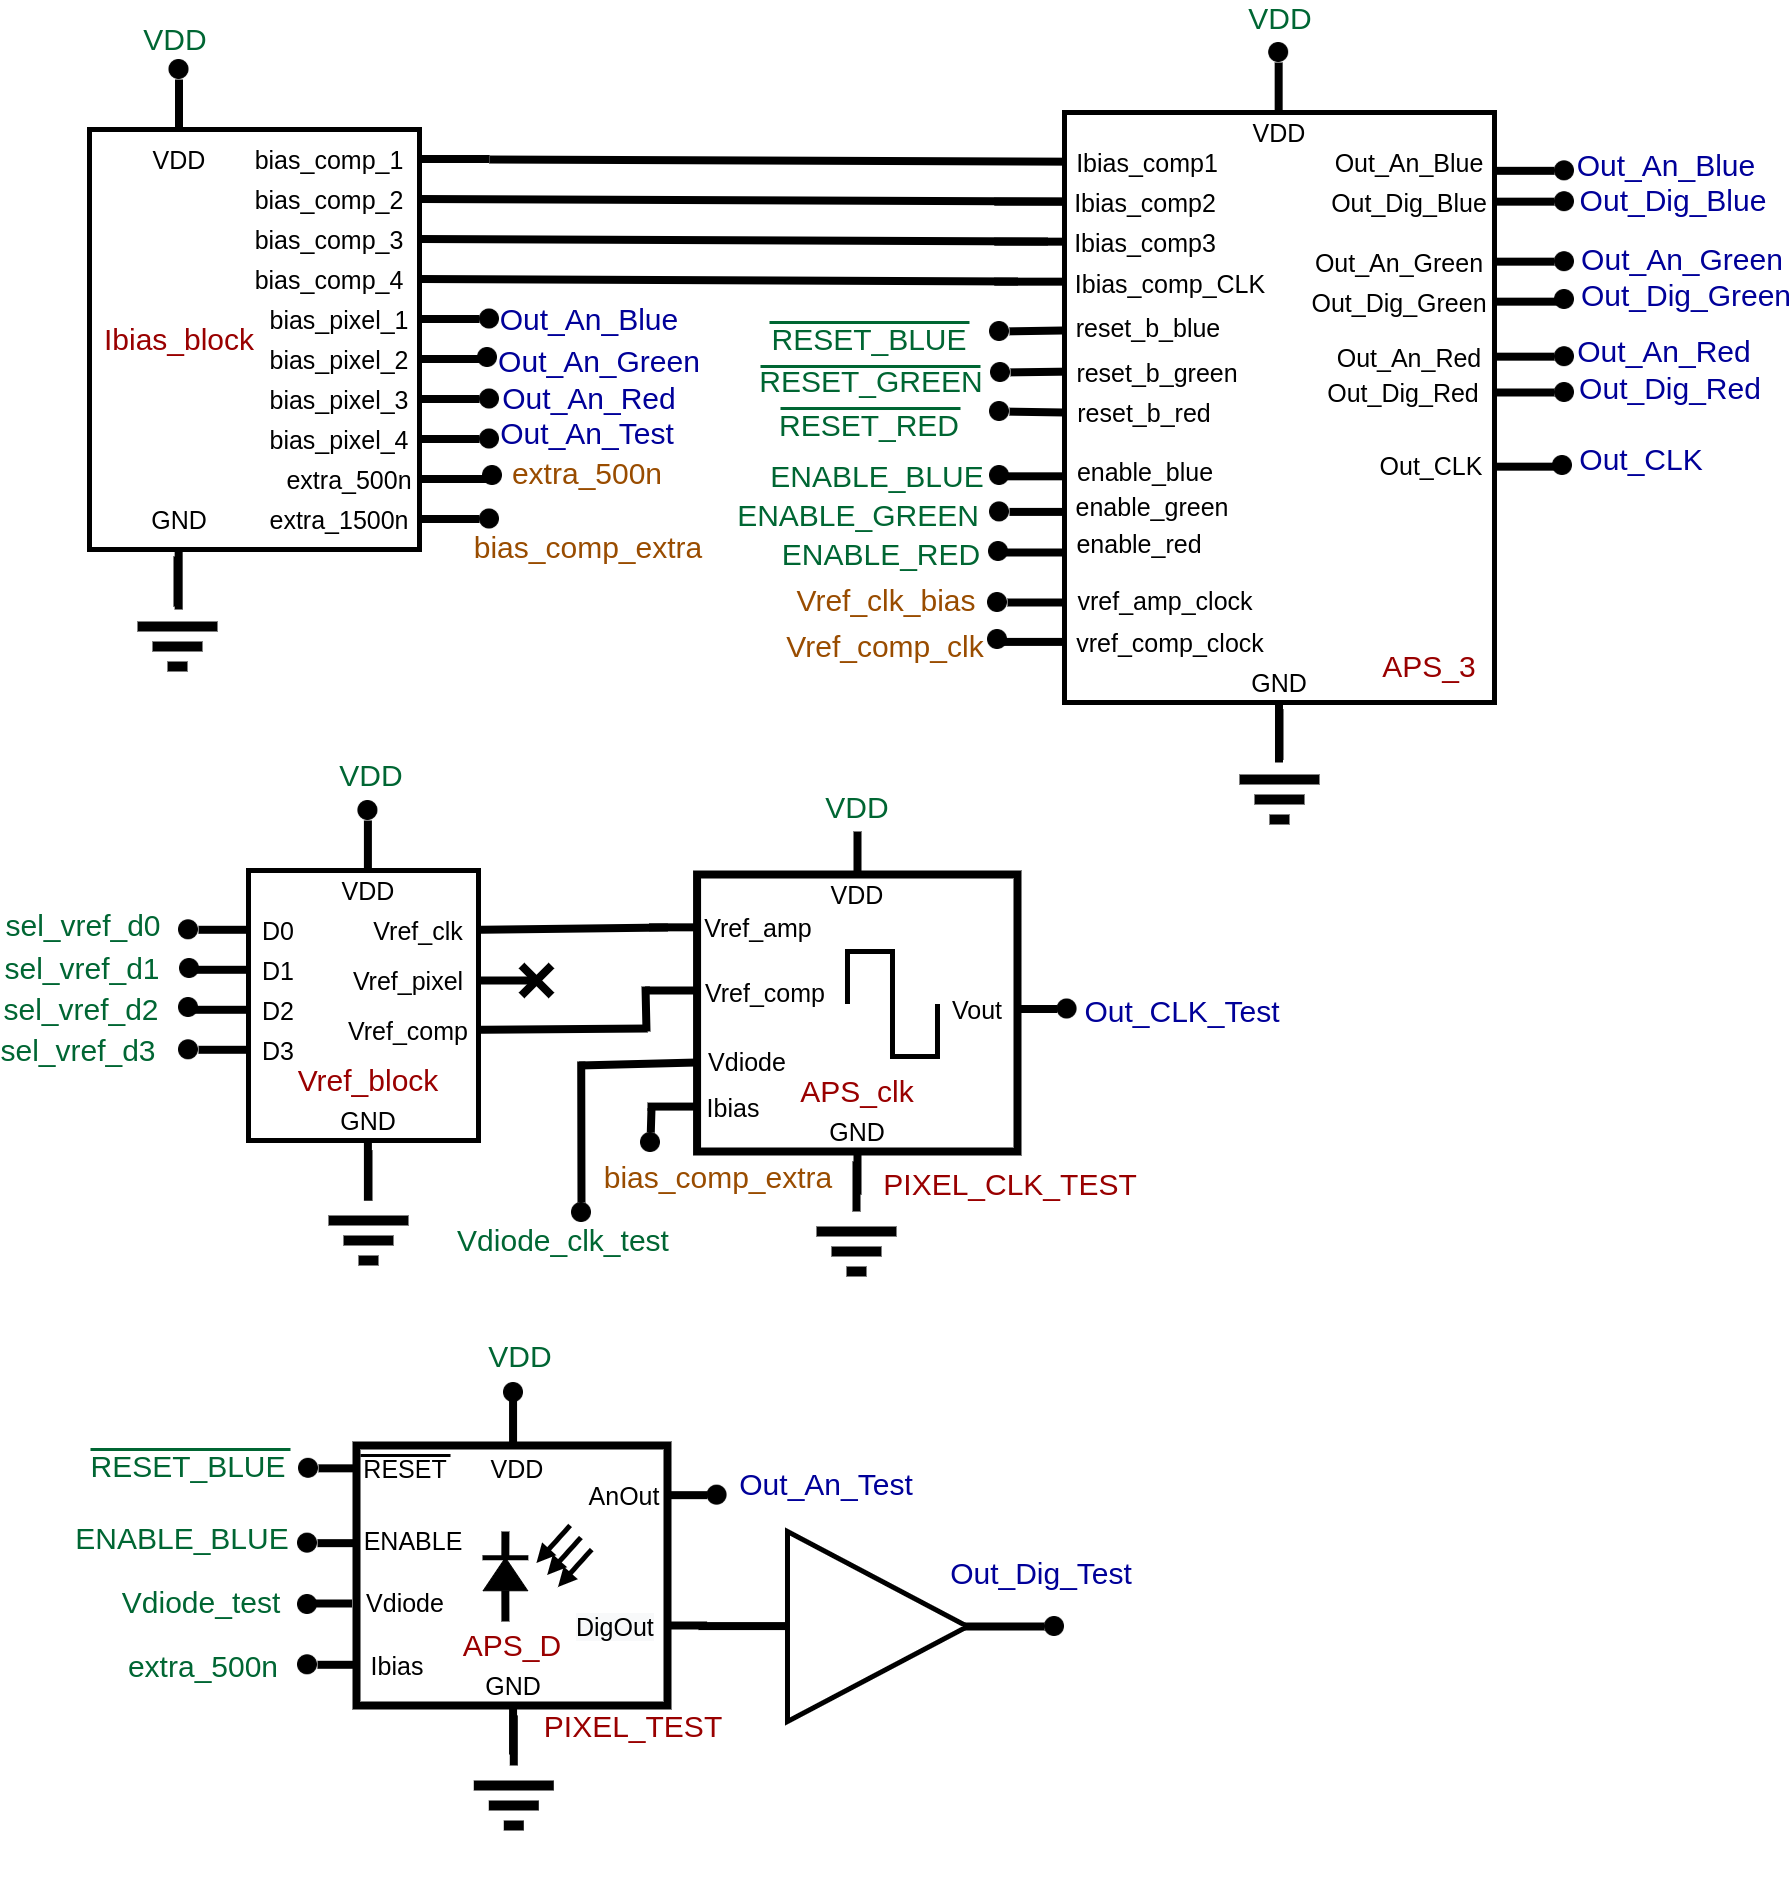
\includegraphics[width=\textwidth]{Circuitos/Complete_Circuit.png}
	\end{center}
	\legend{Fonte: Produzido pelo autor}
\end{figure}

\begin{figure}[!h]
	\caption{\label{fig_circcompletohigh}Representação dos principais blocos presentes no projeto}
	\begin{center}
	    \includegraphics[width=\textwidth]{Imagens/Complete_Circuit_rep.png}
	\end{center}
	\legend{Fonte: Produzido pelo autor}
\end{figure}


O circuito tem a finalidade de processar a informação advinda de tr\^es APS's, constru\'idos de maneira id\^entica em n\'ivel de layout, com a finalidade de abstrair informações de cores advindas de uma fonte luminosa, dos quais podem ser Azul, Verde ou Vermelha. Para que as cores fossem devidamente separadas, são utilizadas películas coloridas externas, que ficam acima de cada respectivo circuito APS de forma a permitir passar somente a informação de uma cor.

Um sinal luminoso de cor branca tamb\'em \'e utilizado no sistema de forma a ser a refer\^encia de rel\'ogio de todos APS's descritos. Esse sinal \'e processado utilizando-se um TIA, do qual \'e gerado um sinal el\'etrico equivalente \`a informação luminosa.

A tecnologia de fabricação utilizada para o desenvolvimento de todos blocos foi a \textit{CMOS TSMC 180nm}. O software utilizado para o projeto do dispositivo foi o \textit{Virtuoso}, desenvolvido pela empresa \textit{Cadence}.

O circuito representado na \autoref{fig_circcompleto} \'e composto por 2 blocos principais, que permitem o processamento advindos da fonte luminosa, al\'em de um circuito APS e um TIA extra. A descrição dos bloco são:

\begin{itemize}
    \item \textit{ibias\_block}: Tem a função de gerar fontes de corrente utilizadas em alguns blocos do circuito.
    
    \item \textit{APS\_3}: Implementa os tr\^es circuitos \textit{APS} descritos, al\'em do circuito TIA. A sa\'ida de cada bloco passa por um comparador de forma a digitalizar o dado, como ser\'a melhor explicitado na \autoref{sec_apsdigitalized}.
    
    \item \textit{Vref\_block} e \textit{PIXEL\_CLK\_TEST}: Estes blocos realizam a implementação de um TIA, por\'em com a adição de um pino extra que possibilita a simulação de uma corrente fotogerada sem necessitar de uma fonte luminosa. Estes blocos serão melhor explicados na \autoref{BlocoTestes}. 
    
    \item \textit{PIXEL\_TEST}: Este bloco realiza a implementação de um APS, com a adição de um pino adicional onde pode ser injetado uma corrente sem a necessidade de uma fonte luminosa. Este bloco será melhor explicado na \autoref{BlocoTestes}.
    
\end{itemize}

A \autoref{tab_circcomp2} mostra a relação de sinais de entrada e sa\'ida presentes no circuito para o processamento dos blocos de teste. A \autoref{tab_circcomp} mostra a relação de sinais de entrada e sa\'ida presentes no circuito, para o processamento dos p\'ixels de cor.

\begin{table}[ht]
  \caption{Descrição dos sinais de entrada e sa\'ida do circuito projetado para os blocos de teste}%
  \label{tab_circcomp2}
  \begin{tabular}{ccl}
  \toprule
   Sinal & Tipo & Descrição \\
   \midrule \midrule
   Vdiode\_test & Entrada & Corrente que simula um potencial no fotodiodo do APS de teste\\
   \midrule
   Vdiode\_clk\_test & Entrada & Corrente que simula um potencial no fotodiodo no TIA de teste\\
   \midrule
   Out\_An\_Test & Sa\'ida & Sinal de tensão anal\'ogico para o APS de teste \\
   \midrule
   Out\_Dig\_Test & Sa\'ida & Sinal de tensão digital para o APS de teste \\
  \midrule
   Out\_CLK\_test & Sa\'ida & Sinal de tensão de rel\'ogio gerado pelo TIA de teste\\
  \bottomrule
\end{tabular}%
  \legend{Fonte: Produzido pelo autor.}
\end{table}

\begin{table}[!h]
\centering
\caption{\label{tab_circcomp}Descrição dos sinais de entrada e sa\'ida do circuito projetado para as cores azul, verde e vermelha}%
  \begin{tabular}{ccll}
  \toprule
   Sinal & Tipo & Descrição & Observação \\
  \midrule \midrule
   RESET\_BLUE & Entrada & \begin{tabular}[l]{@{}l@{}}Sinal de tensão de \textit{RESET}\\ no APS para cor azul\end{tabular}   & Ativo em n\'ivel baixo \\
  \midrule
   RESET\_GREEN & Entrada & \begin{tabular}[l]{@{}l@{}}Sinal de tensão de \textit{RESET}\\ no APS  para cor verde\end{tabular}   & Ativo em n\'ivel baixo \\
  \midrule
   RESET\_RED & Entrada & \begin{tabular}[l]{@{}l@{}}Sinal de tensão de \textit{RESET}\\ no APS  para cor vermelha\end{tabular}   & Ativo em n\'ivel baixo \\
  \midrule
   ENABLE\_BLUE & Entrada & \begin{tabular}[l]{@{}l@{}}Sinal de tensão de \textit{ENABLE}\\ no APS para cor azul\end{tabular}   & Ativo em n\'ivel alto \\
  \midrule
   ENABLE\_GREEN & Entrada & \begin{tabular}[l]{@{}l@{}}Sinal de tensão de \textit{ENABLE}\\ no APS para cor verde\end{tabular}   & Ativo em n\'ivel alto \\
  \midrule
   ENABLE\_RED & Entrada & \begin{tabular}[l]{@{}l@{}}Sinal de tensão de \textit{ENABLE}\\ no APS para cor vermelha\end{tabular}   & Ativo em n\'ivel alto \\
  \midrule
   Out\_An\_Blue & Sa\'ida & \begin{tabular}[l]{@{}l@{}}Sinal de tensão anal\'ogica\\ para cor azul\end{tabular} \\
  \midrule
   Out\_Dig\_Blue & Sa\'ida & \begin{tabular}[l]{@{}l@{}}Sinal de tensão digital\\ para cor azul\end{tabular} \\
  \midrule
   Out\_An\_Green & Sa\'ida & \begin{tabular}[l]{@{}l@{}}Sinal de tensão anal\'ogica\\ para cor verde\end{tabular} \\
  \midrule
   Out\_Dig\_Green & Sa\'ida & \begin{tabular}[l]{@{}l@{}}Sinal de tensão digital\\ para cor verde\end{tabular} \\
  \midrule
   Out\_An\_Red & Sa\'ida & \begin{tabular}[l]{@{}l@{}}Sinal de tensão anal\'ogica\\ para cor vermelha\end{tabular} \\
  \midrule
   Out\_Dig\_Red & Sa\'ida & \begin{tabular}[l]{@{}l@{}}Sinal de tensão digital\\ para cor vermelha\end{tabular} \\
   \midrule
   Out\_CLK & Sa\'ida & \begin{tabular}[l]{@{}l@{}}Sinal de tensão de rel\'ogio\\ gerado pelo TIA\end{tabular}\\
  \bottomrule
\end{tabular}%

\legend{Fonte: Produzido pelo autor.}
\end{table}

\section{Espelhos de Corrente}

Espelhos de Corrente foram necess\'arios para o desenvolvimento de diversos blocos contidos no projeto, e serão especificados nas subseções seguintes. Uma explicação geral sobre o funcionamento e desenvolvimento de espelhos de corrente pode ser vista no \autoref{anexoespelhos}.

\renewcommand{\NomeBloco}{\textit{ibias\_generator}}
\renewcommand{\NomeBlocoNoUnderline}{ibiasgenerator}
\renewcommand{\NomePTab}{tab_\NomeBlocoNoUnderline}
\renewcommand{\NomeSTab}{tab_\NomeBlocoNoUnderline2}
\renewcommand{\NomePFig}{fig_\NomeBlocoNoUnderline}
\renewcommand{\NomeSFig}{fig_\NomeBlocoNoUnderline2}
\renewcommand{\NomeTTab}{tab_\NomeBlocoNoUnderline3}
\renewcommand{\NomeQTab}{tab_\NomeBlocoNoUnderline4}

\subsection{ibias\_generator}
 
O bloco \NomeBloco{}\footnote{Circuito desenvolvido pelo aluno \textit{Daniel Carvalho Lott}, do curso de bacharelado em Engenharia Elétrica da UFMG, no ano de 2020} \'e um espelho de corrente que apresenta uma sa\'ida de 50 $\mu$A. O bloco apresenta as definições de sinais de entrada e sa\'ida referidos na \autoref{\NomeSTab}.

\begin{table}[!h]
\caption{Sinais do bloco \NomeBloco}
\label{\NomeSTab}
\centering
\begin{tabular}{ccl}

    \toprule
    Sinal & Tipo    & Descrição        \\
    \midrule \midrule
    ibias\_1   & Saída   & Fonte de Corrente de 50 $\mu$A \\
    \bottomrule
\end{tabular}
\legend{Fonte: Produzido pelo autor}
\end{table}

O circuito projetado para o bloco \'e demonstrado na \autoref{\NomePFig}.

\begin{figure}[htb]
 \centering
    \centering
    \caption{Circuito CMOS projetado para o bloco \NomeBloco} 
    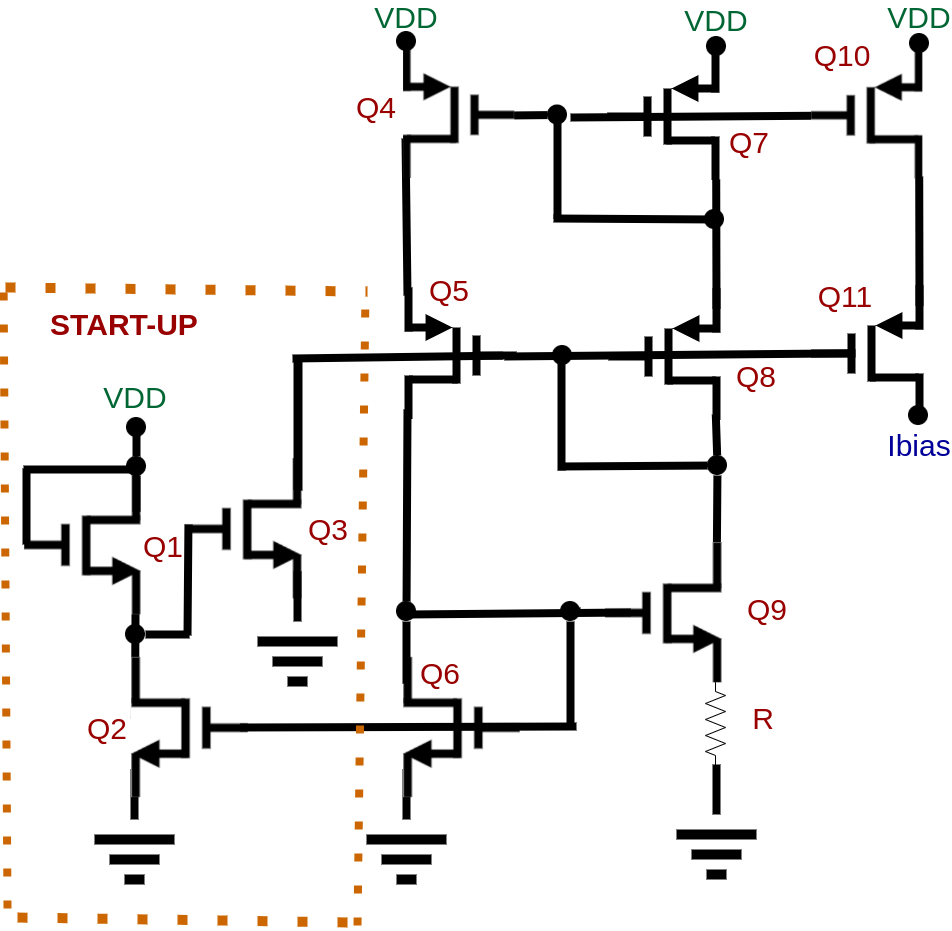
\includegraphics[scale=0.3]{Circuitos/Ibias_generator.png}
    \legend{Fonte: Produzido pelo autor}
    \label{\NomePFig}
\end{figure}

\begin{figure}[htb]
 \centering
    \centering
    \caption{\label{\NomeSFig}Representação em bloco do \NomeBloco}
    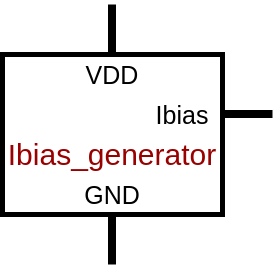
\includegraphics[scale=0.3]{Circuitos/ibias_generator_block.png}
    \legend{Fonte: Produzido pelo autor}
\end{figure}

Os transistores utilizados no bloco apresentam os par\^ametros mostrados na \autoref{\NomeTTab}.

\begin{table}[!h]
\caption{Transistores do Bloco \NomeBloco}
\label{\NomeTTab}
\centering
\begin{tabular}{ccccc}
\toprule
Transistor & W ($\mu$m)  & L ($\mu$m)           & M (n° dispositivos) & S (n° dispositivos)\\
\midrule \midrule
Q1 & 0,3 & 19,995 & 1 & 3\\
\midrule
Q2 & 25 & 0,5 & 2 & 1\\
\midrule
Q3 & 30 & 0,5 & 1 & 1\\
\midrule
Q4, Q7 e Q10 & 35 & 4 & 2 & 1\\
\midrule
Q5, Q8 e Q11 & 25 & 2,5 & 2 & 1\\
\midrule
Q6 & 20 & 4 & 2 & 1\\
\midrule
Q9 & 20 & 4 & 4 & 1\\
\midrule
Q10 & 25 & 2,5 & 2 & 1\\
\midrule
Q11 & 25 & 2,5 & 2 & 1\\
\bottomrule
\end{tabular}
\legend{Fonte: Produzido pelo autor}
\end{table}

O resistor utilizado no bloco apresenta os par\^ametros mostrados na \autoref{\NomeQTab}.

\begin{table}[!h]
\caption{Resistor do bloco \NomeBloco}
\label{\NomeQTab}
\centering
\begin{tabular}{ccccc}
\toprule
Resistor & W ($\mu$m)  & L ($\mu$m) & M (n° dispositivos) & Resist\^encia (k$\Omega$)\\
\midrule \midrule
R & 8 & 29,98 & 2 & 0,569025\\
\bottomrule
\end{tabular}
\legend{Fonte: Produzido pelo autor}
\end{table}

Os transistores \textit{Q6} e \textit{Q9}, juntos aos resistores \textit{R1} e \textit{R2}, t\^em a finalidade de funcionarem como um dreno de corrente referenciados pelos resistores. Os transistores \textit{Q4} e \textit{Q7} t\^em a finalidade de funcionarem como uma fonte de corrente, referenciados pelo dreno de corrente j\'a mencionado. O transistor \textit{Q10} \'e o braço do espelho de corrente do qual fornece a corrente de sa\'ida.

Os transistores \textit{Q5}, \textit{Q8} e \textit{Q11} se apresentam na configuração \textit{Cascode}, que tem o intuito de tornar o espelho de corrente de resposta mais linear, aumentar sua banda e ainda aumentar as suas resist\^encias de entrada e sa\'ida.

Os transistores \textit{Q1}, \textit{Q2} e \textit{Q3} t\^em a função de inicializar o circuito no ponto de operação adequado, j\'a que o circuito tamb\'em apresenta estabilidade quando fornecendo 0 A, sendo necess\'ario evitar essa situação que pode acontecer no momento que o circuito é ligado, estando inicialmente em 0 V.

\renewcommand{\NomeBloco}{\textit{iref\_generator}}
\renewcommand{\NomeBlocoNoUnderline}{irefgenerator}
\renewcommand{\NomePTab}{tab_\NomeBlocoNoUnderline}
\renewcommand{\NomeSTab}{tab_\NomeBlocoNoUnderline2}
\renewcommand{\NomePFig}{fig_\NomeBlocoNoUnderline}
\renewcommand{\NomeSFig}{fig_\NomeBlocoNoUnderline2}
\renewcommand{\NomeTTab}{tab_\NomeBlocoNoUnderline3}
\renewcommand{\NomeQTab}{tab_\NomeBlocoNoUnderline4}

\subsection{iref\_generator}

O bloco \NomeBloco{}\footnote{Circuito desenvolvido por \textit{Dalton Martini Colombo}, orientador do trabalho aqui apresentado} \'e um espelho de corrente que apresenta algumas sa\'idas como fonte e outras em dreno de corrente. O bloco apresenta as definições de sa\'ida referidos na \autoref{\NomeSTab}.

\begin{table}[!h]
\caption{Sinais do bloco \NomeBloco}
\label{\NomeSTab}
\centering
\begin{tabular}{ccl}

    \toprule
    Sinal & Tipo    & Descrição        \\
    \midrule \midrule
    iref1\_src   & Saída   & Fonte de Corrente de 0.5 $\mu$A \\
    \midrule
    iref2\_src   & Saída   & Fonte de Corrente de 0.5 $\mu$A \\
    \midrule
    iout\_test   & Saída   & Fonte de Corrente de 1.5 $\mu$A \\
    \midrule
    iref1\_sink   & Saída   & Dreno de Corrente de 0.5 $\mu$A \\
    \midrule
    iref2\_sink   & Saída   & Dreno de Corrente de 0.5 $\mu$A \\
    \bottomrule
\end{tabular}
\legend{Fonte: Produzido pelo autor}
\end{table}

O circuito projetado para o bloco \'e demonstrado na \autoref{\NomePFig}.

\begin{figure}[htb]
 \centering
    \centering
    \caption{Circuito CMOS projetado para o bloco \NomeBloco} 
    \includegraphics[scale=0.3]{Circuitos/iref_generator.png}
    \legend{Fonte: Produzido pelo autor}
    \nota{Nem todos transistores são representados na imagem. \emph{Q17}, \emph{Q18}, \emph{Q19} e \emph{Q20} são transistores replicados para cada sa\'ida \emph{IrefX\_src} e \emph{IrefY\_sink}, onde \emph{X} e \emph{Y} são os identificadores de cada sa\'ida}
    \label{\NomePFig}
\end{figure}

\begin{figure}[htb]
 \centering
    \centering
    \caption{\label{\NomeSFig}Representação em bloco do \NomeBloco}
    \includegraphics[scale=0.3]{Circuitos/iref_generator_block.png}
    \legend{Fonte: Produzido pelo autor}
\end{figure}

Os transistores utilizados no bloco apresentam os par\^ametros mostrados na \autoref{\NomeTTab}.

\begin{table}[!h]
\caption{Transistores do Bloco \NomeBloco}
\label{\NomeTTab}
\centering
\begin{tabular}{ccccc}
\toprule
Transistor & W ($\mu$m)  & L ($\mu$m)  & M (n° dispositivos) & S (n° dispositivos)\\
\midrule \midrule

\midrule
Q1                                   & 0,3    & 19,995 & 1                   & 3                   \\
\midrule
Q2                                   & 35     & 0,18   & 2                   & 1                   \\
\midrule
Q3 e Q4                              & 15     & 0,18   & 1                   & 1                   \\
\midrule
Q5                                   & 10     & 15     & 1                   & 6                   \\
\midrule
\begin{tabular}[c]{@{}c@{}}Q6, Q9, Q10,\\ Q13, Q19 e Q20\end{tabular}          & 4      & 19,995 & 1                   & 2                   \\
\midrule
\begin{tabular}[c]{@{}c@{}}Q7, Q8, Q11, Q12,\\ Q15, Q17a¹ e Q18a¹\end{tabular} & 10     & 15   & 2                   & 1                   \\
\midrule
Q14                                  & 4      & 19,995 & 10                  & 1                   \\
\midrule
Q16                                  & 4      & 19,995 & 1                   & 6 \\
\midrule
Q17b² e Q18b²                                                                  & 10     & 15     & 6                   & 1                  \\
\bottomrule
\end{tabular}
\legend{Fonte: Produzido pelo autor}
\legend{¹ Q17a e Q18a são os transistores referentes \`as sa\'idas iref1\_src e iref2\_src\\
² Q17b e Q18b são os transistores referentes \`a sa\'ida iout\_test}
\end{table}

O resistor \emph{R} utilizado no bloco apresenta os par\^ametros mostrado na \autoref{\NomeQTab}.

\begin{table}[!h]
\caption{Resistor do bloco \NomeBloco}
\label{\NomeQTab}
\centering
\begin{tabular}{cccc}
\toprule
Resistor & W ($\mu$m)  & L ($\mu$m) & Resist\^encia (k$\Omega$)\\
\midrule \midrule
R & 3 & 404,4 & 141,996\\
\bottomrule
\end{tabular}
\legend{Fonte: Produzido pelo autor}
\end{table}

Os transistores \emph{Q6} e \emph{Q9}, juntos ao resistor R, t\^em a finalidade de funcionarem como um dreno de corrente referenciados pelo resistor. Os transistores \emph{Q4} e \emph{Q7} t\^em a finalidade de funcionarem como uma fonte de corrente, referenciados pelo dreno de corrente j\'a mencionado. O transistor \emph{Q10} \'e o braço do espelho de corrente do qual fornece a corrente de sa\'ida.

Os transistores \emph{Q5}, \emph{Q8} e \emph{Q11} se apresentam na configuração \emph{Cascode}, que tem o intuito de tornar o espelho de corrente de resposta mais linear, aumentar sua banda e ainda aumentar as suas resist\^encias de entrada e sa\'ida.

Os transistores \emph{Q1}, \emph{Q2} e \emph{Q3} t\^em a função de inicializarem o circuito no ponto de operação adequado, j\'a que o circuito tamb\'em apresenta estabilidade quando fornecendo 0 A, sendo necess\'ario evitar essa situação.

\renewcommand{\NomeBloco}{\textit{current\_mirror\_nmos}}
\renewcommand{\NomeBlocoNoUnderline}{curmirnmosb}
\renewcommand{\NomePTab}{tab_\NomeBlocoNoUnderline}
\renewcommand{\NomeSTab}{tab_\NomeBlocoNoUnderline2}
\renewcommand{\NomePFig}{fig_\NomeBlocoNoUnderline}
\renewcommand{\NomeSFig}{fig_\NomeBlocoNoUnderline2}
\renewcommand{\NomeTTab}{tab_\NomeBlocoNoUnderline3}
\renewcommand{\NomeQTab}{tab_\NomeBlocoNoUnderline4}

\subsection{current\_mirror\_nmos}

O bloco \NomeBloco{} cont\'em alguns braços utilizados como dreno de corrente para outras partes do circuito, sendo todos valores iguais \`a corrente de refer\^encia. O bloco apresenta as definições de sinais de entrada e sa\'ida referidos na \autoref{\NomeSTab}.

\begin{table}[!h]
\caption{Sinais do bloco \NomeBloco}
\label{\NomeSTab}
\centering
\begin{tabular}{ccl}

    \toprule
    Sinal & Tipo    & Descrição        \\
    \midrule \midrule
    Iref\_bias   & Entrada   &  Corrente de refer\^encia para os braços \\
    \midrule
    Iref\_A   & Saída   &  Braço 1 \\
    \midrule
    Iref\_B   & Saída   &  Braço 2 \\
    \midrule
    Iref\_C   & Saída   &  Braço 3 \\
    \midrule
    Iref\_D   & Saída   &  Braço 4 \\
    \midrule
    Iref\_E   & Saída   &  Braço 5 \\
    \bottomrule
\end{tabular}
\legend{Fonte: Produzido pelo autor}
\end{table}

O circuito projetado para o bloco \'e demonstrado na \autoref{\NomePFig}.

\begin{figure}[htb]
 \centering
    \centering
    \caption{Circuito CMOS projetado para o bloco \NomeBloco} 
    \includegraphics[scale=0.3]{Circuitos/current_mirror.png}
    \legend{Fonte: Produzido pelo autor}
    \label{\NomePFig}
\end{figure}

\begin{figure}[htb]
 \centering
    \centering
    \caption{\label{\NomeSFig}Representação em bloco do \NomeBloco} 
    \includegraphics[scale=0.3]{Circuitos/current_mirror_block.png}
    \legend{Fonte: Produzido pelo autor}
\end{figure}

Os transistores utilizados no bloco apresentam os par\^ametros mostrados na \autoref{\NomeTTab}.

\begin{table}[!h]
\caption{Transistores do Bloco \NomeBloco}
\label{\NomeTTab}
\centering
\begin{tabular}{ccccc}
\toprule
Transistor & W ($\mu$m)  & L ($\mu$m)           & M (n° dispositivos) & S (n° dispositivos)\\
\midrule \midrule
\begin{tabular}[c]{@{}c@{}}Q1, Q2, Q3,\\
Q4, Q5 e Q6\end{tabular} & 5 & 6 & 2 & 1\\
\bottomrule
\end{tabular}
\legend{Fonte: Produzido pelo autor}
\end{table}
\renewcommand{\NomeBloco}{\textit{APS}}
\renewcommand{\NomeBlocoNoUnderline}{blocoAPS}
\renewcommand{\NomePTab}{tab_\NomeBlocoNoUnderline}
\renewcommand{\NomeSTab}{tab_\NomeBlocoNoUnderline2}
\renewcommand{\NomePFig}{fig_\NomeBlocoNoUnderline}
\renewcommand{\NomeSFig}{fig_\NomeBlocoNoUnderline2}
\renewcommand{\NomeTTab}{tab_\NomeBlocoNoUnderline3}
\renewcommand{\NomeQTab}{tab_\NomeBlocoNoUnderline4}

\section{APS}

O bloco \NomeBloco{} implementa o circuito apresentado na \autoref{fig_APS}. O bloco apresenta as definições de sinais de entrada e sa\'ida referidos na \autoref{\NomeSTab}.

\begin{table}[!h]
\label{\NomeSTab}
\begin{tabular}{ccll}
\toprule
Sinal      & Tipo    & \multicolumn{1}{c}{Descrição}                                                          & \multicolumn{1}{c}{Observação}                                                                               \\
\midrule \midrule
RESET      & Entrada & Sinal de tensão de RESET no APS                                                        & Ativo em nível baixo                                                                                         \\
\midrule
ENABLE     & Entrada & Sinal de tensão de ENABLE no APS                                                       & Ativo em nível alto                                                                                          \\
\midrule
SELECT     & Entrada & Sinal de tensão de SELECT no APS                                                       & \begin{tabular}[c]{@{}l@{}}Ativo em nível alto.\\ Mantido internamente \\ em nível alto\end{tabular} \\
\midrule
Ibias\_clk & Entrada & Dreno de Corrente do bloco (500 nA)                                                    &                                                                                                              \\
\midrule
Vout       & Saída   & \begin{tabular}[c]{@{}l@{}}Sinal de tensão analógica produzido\\ pelo APS\end{tabular} &    \\
\bottomrule
\end{tabular}
\legend{Fonte: Produzido pelo autor.}
\end{table}

A representação em bloco do circuito projetado é dado na \autoref{\NomeSFig}.

\begin{figure}[!h]
 \centering
    \centering
    \caption{\label{\NomeSFig}Representação em bloco do \NomeBloco} 
    \includegraphics[scale=0.3]{Circuitos/APS_block.png}
    \legend{Fonte: Produzido pelo autor}
\end{figure}

Os transistores utilizados no bloco apresentam os par\^ametros mostrados na \autoref{\NomeTTab}.

\begin{table}[!h]
\caption{Transistores do bloco \NomeBloco}
\label{\NomeTTab}
\centering
\begin{tabular}{ccccc}
\toprule
Transistor & W ($\mu$m)  & L ($\mu$m)           & M (n° dispositivos) & S (n° dispositivos)\\
\midrule \midrule
T\textsubscript{buffer} & 15 & 0,75 & 1 & 1\\
\midrule
T\textsubscript{reset} & 4 & 0,18 & 1 & 1\\
\midrule
T\textsubscript{select} & 10 & 0,18 & 2 & 2\\
\bottomrule
\end{tabular}
\legend{Fonte: Produzido pelo autor}
\end{table}

O fotodiodo utilizado no bloco apresenta os par\^ametros mostrados na \autoref{\NomeQTab}. $W$ é a largura do fotodiodo. $L$ é o comprimento do fotodiodo.

\begin{table}[!h]
\caption{Fotodiodo do bloco \NomeBloco}
\label{\NomeQTab}
\centering
\begin{tabular}{cccc}
\toprule
Nome & W ($\mu$m)  & L ($\mu$m) & Área ($\mu$m²)\\
\midrule \midrule
Fotodiodo & 25 & 25 & 625\\
\bottomrule
\end{tabular}
\legend{Fonte: Produzido pelo autor}
\end{table}

Informações referentes à $T\textsubscript{enable}$ podem ser vistas no \autoref{portatg}.
\renewcommand{\NomeBloco}{\textit{APS\_digitalized}}
\renewcommand{\NomeBlocoNoUnderline}{apsdigitalized}
\renewcommand{\NomePTab}{tab_\NomeBlocoNoUnderline}
\renewcommand{\NomeSTab}{tab_\NomeBlocoNoUnderline2}
\renewcommand{\NomePFig}{fig_\NomeBlocoNoUnderline}
\renewcommand{\NomeSFig}{fig_\NomeBlocoNoUnderline2}
\renewcommand{\NomeTTab}{tab_\NomeBlocoNoUnderline3}
\renewcommand{\NomeQTab}{tab_\NomeBlocoNoUnderline4}

\section{APS\_digitalized}
\label{sec_apsdigitalized}

O \textit{APS\_digitalized} \'e o circuito respons\'avel por digitalizar o sinal gerado pelo APS descrito na \autoref{section:APS}. O bloco apresenta as definições de sinais de entrada e sa\'ida referidos na \autoref{\NomeSTab}.

\begin{table}[!h]
\caption{Sinais do bloco \NomeBloco}
\label{\NomeSTab}
\centering
\begin{tabular}{ccll}

    \toprule
    Sinal & Tipo    & Descrição & Observação        \\
    \midrule \midrule
    RESET   & Entrada   & Sinal de tensão de RESET no APS & Ativo em nível baixo\\
    \midrule
    ENABLE   & Entrada   & Sinal de tensão de ENABLE no APS & Ativo em nível alto\\
    \midrule
    Vref   & Entrada   & \begin{tabular}[l]{@{}l@{}}Tensão de refer\^encia utilizada pelo\\ \textit{Comparador}\end{tabular} \\
    \midrule
    Ibias   & Entrada   & Corrente de polarização do comparador \\
    \midrule
    AnOut   & Saída   & \begin{tabular}[l]{@{}l@{}}Sinal de tensão anal\'ogica produzido\\ pelo APS\end{tabular} \\
    \midrule
    DigOut   & Saída   & \begin{tabular}[l]{@{}l@{}}Sinal de tensão digital produzido\\ pelo \textit{Comparador}\end{tabular} \\
    \bottomrule
\end{tabular}
\legend{Fonte: Produzido pelo autor}
\end{table}

O circuito projetado para o bloco \'e demonstrado nas figuras \ref{repblocoAPS} e \ref{repblocoAPS2}.

\begin{figure}[!h]
 \centering
    \centering
    \caption{Circuito CMOS projetado para o bloco \NomeBloco com o circuito do APS explicito} 
    \includegraphics[scale=0.3]{Circuitos/APS_digitalized_rep.png}
    \legend{Fonte: Produzido pelo autor}
    \label{repblocoAPS}
\end{figure}

\begin{figure}[!h]
 \centering
    \centering
    \caption{Circuito CMOS projetado para o bloco \NomeBloco} 
    \includegraphics[scale=0.3]{Circuitos/APS_digitalized.png}
    \legend{Fonte: Produzido pelo autor}
    \label{repblocoAPS2}
\end{figure}

\begin{figure}[!h]
 \centering
    \centering
    \caption{\label{\NomeSFig}Representação em bloco do \NomeBloco}
    \includegraphics[scale=0.3]{Circuitos/APS_digitalized_block.png}
    \legend{Fonte: Produzido pelo autor}
\end{figure}

A sa\'ida digital do bloco funciona realizando uma comparação entre uma tensão de refer\^encia chamada de \textit{Vref} e a sa\'ida anal\'ogica do APS, chamada de \textit{AnOut}. Quando o valor de \textit{Vref} for maior do que o de \textit{AnOut}, o comparador ir\'a saturar e apresentar um sinal aproximadamente igual a VDD, interpretada como n\'ivel l\'ogico '1'. Quando o valor de \textit{Vref} for menor ou igual do que o de \textit{AnOut}, o comparador ir\'a apresentar um sinal aproximadamente igual a GND em sua sa\'ida, interpretada como n\'ivel l\'ogico '0'.

Utilizando o elemento comparador, podemos ajustar para que a sa\'ida retorne '0' apenas quando for atingido um valor limiar controlado. Como sabemos que a intensidade da corrente fotogerada depende da intensidade da luz captada pelo fotodiodo (\autoref{secao_fotodiodo}), podemos deduzir a informação sobre intensidade luminosa verificando em quanto tempo demora para que se mude de n\'ivel l\'ogico '1' para '0' durante o Est\'agio 2, considerando que o nó $V_{cn}$ apresentava o valor de VDD, que equivale à $AnOut$ apresentar o máximo valor em sua saída (\autoref{eq_voutfinal}). Considerando o atraso no comparador nulo, e desprezando-se as resistências das chaves no bloco APS, podemos utilizar as equações \ref{eq_responsividade}, \ref{eq_modEletFotIl} e \ref{eq_voutfinal} para se obter a \autoref{eq_apsd}.

\begin{equation}
    \label{eq_apsd}
    P_{FD} = \frac{(AnOut_0-V_{ref})(C_{j}+C_{cn})}{R_{\lambda}t_{1-0}}
\end{equation}

Onde:

\begin{itemize}

    \item \textit{P$_{FD}$} \'e a pot\^encia \'optica presente no fotodiodo [\textit{W}]
    \item $AnOut_0$ \'e o valor do nó $AnOut$ no momento que inicia o Período de Integração [$V$]
    \item \textit{$V_{ref}$} \'e a tensão de refer\^encia do comparador [$V$]
    \item \textit{$C_j$} \'e a capacit\^ancia de junção do fotodiodo [\textit{F}]
    \item \textit{$C_{cn}$} \'e a capacit\^ancia do n\'o central do APS [\textit{F}]
    \item $R_{\lambda}$ \'e a responsividade para o comprimento de onda detectado no fotodiodo [$A.W^{-1}$]
    \item $t_{1\_0}$ \'e o tempo do qual o n\'ivel l\'ogico demorou para mudar de '1' para '0', a partir do momento que se inicia o Estágio 2, representado na \autoref{figurataps}, equivalente ao tempo para que a tensão de saída do APS seja igual a Vref [\textit{s}]
    
\end{itemize}

\begin{figure}[!h]
 \centering
    \centering
    \caption{\label{figurataps}Comparação da saída do APS com a tensão de referência do comparador do $APS\_digitalized$ \NomeBloco} 
    \includegraphics[scale=0.3]{Imagens/Graficot.png}
    \legend{Fonte: Produzido pelo autor}
    \label{\NomePFig}
\end{figure}

\renewcommand{\NomeBloco}{\textit{APS\_pixel\_clk}}
\renewcommand{\NomeBlocoNoUnderline}{apspixelclk}
\renewcommand{\NomePTab}{tab_\NomeBlocoNoUnderline}
\renewcommand{\NomeSTab}{tab_\NomeBlocoNoUnderline2}
\renewcommand{\NomePFig}{fig_\NomeBlocoNoUnderline}
\renewcommand{\NomeSFig}{fig_\NomeBlocoNoUnderline2}
\renewcommand{\NomeTTab}{tab_\NomeBlocoNoUnderline3}
\renewcommand{\NomeQTab}{tab_\NomeBlocoNoUnderline4}

\section{APS\_pixel\_clk}

O \NomeBloco{}\footnote{Circuito esquemático desenvolvido por \textit{Dalton Martini Colombo}} \'e o bloco respons\'avel por processar e digitalizar o sinal gerado pelo \textit{TIA}. A intenção de uso do \textit{TIA} \'e que ele seja o respons\'avel por captar um sinal luminoso com frequ\^encia bem definida, e o sinal el\'etrico gerado, em forma de pulsos quadrados, sirva de refer\^encia de rel\'ogio para todos os circuitos APS utilizados para detecção de cor. O bloco portanto tem como responsabilidade gerar um sinal digital de frequ\^encia igual a do sinal luminoso captado. O bloco apresenta as definições de sinais de entrada e sa\'ida referidos na \autoref{\NomeSTab}.

\begin{table}[!h]
\caption{Sinais do bloco \NomeBloco}
\label{\NomeSTab}
\centering
\begin{tabular}{cclc}

    \toprule
    Sinal & Tipo    & Descrição  & Observação\\
    \midrule \midrule
    Vref\_comp   & Entrada   & Tensão de refer\^encia utilizada pelo comparador &  1,15 V\\
    \midrule
    Vref\_amp   & Entrada   & Tensão de refer\^encia utilizada para o TIA &  0,77 V\\
    \midrule
    Ibias   & Entrada   & Corrente de polarização do comparador & 500 nA \\
    \midrule
    Vout   & Saída   & Sinal digital produzido pelo Comparador\\
    \bottomrule
\end{tabular}
\legend{Fonte: Produzido pelo autor}
\end{table}

A \autoref{TIAsimplifC} mostra o circuito projetado de maneira simplificada. O circuito completo projetado para o bloco \'e demonstrado na \autoref{\NomePFig}.

\begin{figure}[!h]
 \centering
    \centering
    \caption{Circuito CMOS simplificado projetado para o bloco \NomeBloco} 
    \includegraphics[scale=0.6]{Circuitos/TIA_ref.png}
    \label{TIAsimplifC}
    \legend{Fonte: Produzido pelo autor}
\end{figure}

\begin{figure}[!h]
 \centering
    \centering
    \caption{Circuito CMOS projetado para o bloco \NomeBloco} 
    \includegraphics[scale=0.3]{Circuitos/APS_clk.png}
    \label{\NomePFig}
    \legend{Fonte: Produzido pelo autor}
\end{figure}

\begin{figure}[!h]
 \centering
    \centering
    \caption{\label{\NomeSFig}Representação em bloco do \NomeBloco}
    \includegraphics[scale=0.3]{Circuitos/APS_clk_block.png}
    \legend{Fonte: Produzido pelo autor}
\end{figure}

O circuito tem funcionamento similar ao do apresentado no bloco \textit{APS\_digitalized}, por\'em com apenas a sa\'ida digital sendo considerada e sendo utilizado um $TIA$ ao inv\'es de um \textit{APS}. A corrente de polarização do par diferencial \'e gerada pelo bloco \textit{Ibias\_generator}, contido no bloco.

Uma resist\^encia $R$ de ganho \'e utilizada, com valor apresentado na \autoref{\NomeQTab}. $W$ é a largura do resistor. $L$ é o comprimento do resistor.

\begin{table}[!h]
\caption{Resistor do bloco \NomeBloco}
\label{\NomeQTab}
\centering
\begin{tabular}{cccc}
\toprule
Resistor & W ($\mu$m)  & L ($\mu$m) & Resist\^encia (M$\Omega$)\\
\midrule \midrule
R & 1,68 & 39486,3 & 25\\
\bottomrule
\end{tabular}
\legend{Fonte: Produzido pelo autor}
\end{table}

O fotodiodo utilizado no bloco apresenta os par\^ametros mostrados na \autoref{\NomeTTab}. $W$ é a largura do fotodiodo. $L$ é o comprimento do fotodiodo.

\begin{table}[!h]
\caption{Fotodiodo do bloco \NomeBloco}
\label{\NomeTTab}
\centering
\begin{tabular}{cccc}
\toprule
Nome & W ($\mu$m)  & L ($\mu$m) & Área ($\mu$m²)\\
\midrule \midrule
Fotodiodo & 25 & 25 & 625\\
\bottomrule
\end{tabular}
\legend{Fonte: Produzido pelo autor}
\end{table}

Com base na \autoref{eqCTIA2}, a \autoref{eq_TIAblock} descreve $V_{p}$, que \'e comparada com \textit{Vref\_comp} e então utilizada para gerar o sinal de sa\'ida.

\begin{equation}
    \label{eq_TIAblock}
    V_{p} = RI_{PH}
\end{equation}

Onde:

\begin{itemize}

    \item \textit{$V_{P}$} \'e a tensão no ramo positivo do comparador [$V$]
    \item \textit{$I_{PH}$} \'e a corrente fotogerada [$A$]
    
\end{itemize}
\renewcommand{\NomeBloco}{\textit{vref\_generator}}
\renewcommand{\NomeBlocoNoUnderline}{vrefgenerator}
\renewcommand{\NomePTab}{tab_\NomeBlocoNoUnderline}
\renewcommand{\NomeSTab}{tab_\NomeBlocoNoUnderline2}
\renewcommand{\NomePFig}{fig_\NomeBlocoNoUnderline}
\renewcommand{\NomeSFig}{fig_\NomeBlocoNoUnderline2}
\renewcommand{\NomeTTab}{tab_\NomeBlocoNoUnderline3}
\renewcommand{\NomeQTab}{tab_\NomeBlocoNoUnderline4}

\section{vref\_generator}

O \textit{\NomeBloco}\footnote{Circuito esquemático desenvolvido por \textit{Dalton Martini Colombo}} \'e o bloco respons\'avel por gerar todas as tensões de refer\^encia utilizados nos outros blocos do circuito. O bloco apresenta as definições de sinais de entrada e sa\'ida referidos na \autoref{\NomeSTab}.

\begin{table}[!h]
\caption{Sinais do bloco \NomeBloco}
\label{\NomeSTab}
\centering
\begin{tabular}{ccl}

    \toprule
    Sinal & Tipo    & Descrição      \\
    \midrule \midrule
    Ibias   & Entrada   & Corrente de polarização do bloco \textit{Par Diferencial} \\
    \midrule
    V\_extra   & Saída   & Tensão de refer\^encia de 1,15 V \\
    \midrule
    Vref\_plus   & Saída   & Tensão de refer\^encia de 1,02 V \\
    \midrule
    Vref   & Saída   & Tensão de refer\^encia de 898,45 mV \\
    \midrule
    y1   & Saída   & Tensão de refer\^encia de 772,67 mV \\
    \midrule
    y2   & Saída   & Tensão de refer\^encia de 646,89 mV \\
    \midrule
    y3   & Saída   & Tensão de refer\^encia de 521,1 mV \\
    \midrule
    y4  & Saída   & Tensão de refer\^encia de 395,32 mV  \\
    \midrule
    y5   & Saída   & Tensão de refer\^encia de 269,54 mV \\
    \midrule
    y6   & Saída   & Tensão de refer\^encia de 143,75 mV \\
    \bottomrule
\end{tabular}
\legend{Fonte: Produzido pelo autor}
\end{table}

O circuito projetado para o bloco \'e demonstrado na \autoref{\NomePFig}.

\begin{figure}[htb]
 \centering
    \centering
    \caption{\label{\NomePFig}Circuito CMOS projetado para o bloco \NomeBloco} 
    \includegraphics[scale=0.3]{Circuitos/vref_generator.png}
    \legend{Fonte: Produzido pelo autor}
\end{figure}

\begin{figure}[htb]
 \centering
    \centering
    \caption{\label{\NomeSFig}Representação em bloco do \NomeBloco}
    \includegraphics[scale=0.3]{Circuitos/vref_generator_block.png}
    \legend{Fonte: Produzido pelo autor}
\end{figure}

Os transistores utilizados no bloco \NomeBloco{} apresentam os par\^ametros mostrados na \autoref{\NomeTTab}.

\begin{table}[!h]
\caption{Transistores do Bloco \NomeBloco}
\label{\NomeTTab}
\centering
\begin{tabular}{ccccc}
\toprule
Transistor & W ($\mu$m)  & L ($\mu$m)           & M (n° dispositivos) & S (n° dispositivos)\\
\midrule \midrule
Q1 e Q2 & 0,5 & 19,995 & 1 & 1\\
\midrule
Q3 & 20 & 0,18 & 1 & 1\\
\midrule
Q4 & 2 & 0,18 & 1 & 1\\
\midrule
Q5, Q6 e Q7 & 20 & 16 & 4 & 1\\
\midrule
Qb1 (PNP) & 5 & 5 & 1 & 1\\
\midrule
Qb2 (PNP) & 5 & 5 & 8 & 1\\
\bottomrule
\end{tabular}
\legend{Fonte: Produzido pelo autor}
\end{table}

Os resistores utilizados no bloco \NomeBloco{} apresentam os par\^ametros mostrados na \autoref{\NomeQTab}.

\begin{table}[!h]
\caption{Resistores do bloco \NomeBloco}
\label{\NomeQTab}
\centering
\begin{tabular}{cccccc}
\toprule
Resistor & \begin{tabular}[c]{@{}c@{}}W \\($\mu$m)\end{tabular}   & \begin{tabular}[c]{@{}c@{}}L \\($\mu$m)\end{tabular}  & \begin{tabular}[c]{@{}c@{}}Resist\^encia\\ (k$\Omega$)\end{tabular} & \begin{tabular}[c]{@{}c@{}}M\\(n° dispositivos)\end{tabular} & \begin{tabular}[c]{@{}c@{}}S \\(n° dispositivos)\end{tabular}\\
\midrule \midrule
R1 e R2 & 2 & 18,85 & 10,1024 & 1 & 10\\
\midrule
\begin{tabular}[c]{@{}c@{}}R\_amp, R3, R4,\\ R5, R6, R7, \\ R8, R9, R10, \\ R11\end{tabular} & 2 & 18,85 & 10,1024 & 1 & 1\\
\midrule
R12 & 2 & 18,85 & 10,1024 & 7 & 1\\
\bottomrule
\end{tabular}
\legend{Fonte: Produzido pelo autor}
\end{table}

O dispositivo funciona produzindo uma corrente de refer\^encia extremamente est\'avel, utilizando um amplificador operacional e realimentação. O braço \textit{Q7} utiliza dessa corrente como refer\^encia para gerar uma corrente que alimenta alguns resistores, que geram os potenciais de refer\^encia desejados.

\renewcommand{\NomeBloco}{\emph{vref\_block}}
\newcommand{\NomeBlocoA}{vrefblock}
\renewcommand{\NomePTab}{tab_\NomeBlocoA}
\renewcommand{\NomeSTab}{tab_\NomeBlocoA2}
\renewcommand{\NomePFig}{fig_\NomeBlocoA}
\renewcommand{\NomeSFig}{fig_\NomeBlocoA2}
\renewcommand{\NomeTTab}{tab_\NomeBlocoA3}

\section{vref\_block}

O bloco \NomeBloco{} tem a finalidade de conter o bloco \emph{vref\_generator}, mais o bloco respons\'avel por gerar a corrente que o polariza. O bloco apresenta as definições de sinais de entrada e sa\'ida referidos na \autoref{\NomeSTab}.

\begin{table}[!h] 
\caption{Sinais do bloco \NomeBloco}
\label{\NomeSTab}
\centering
\begin{tabular}{ccll}

    \toprule
    Sinal & Tipo    & Descrição & Bloco de utilização     \\
    \midrule \midrule
    V\_extra   & Saída   & Tensão de refer\^encia 1 & APS\_pixel\_clk \\
    \midrule
    Vref\_plus   & Saída   & Tensão de refer\^encia 2 & APS\_digitalized\\
    \midrule
    Vref   & Saída   & Tensão de refer\^encia 3 & APS\_digitalized \\
    \midrule
    Vref\_minus   & Saída   & Tensão de refer\^encia 4 & APS\_pixel\_clk \\
    \midrule
    Vref\_minus2   & Saída   & Tensão de refer\^encia 5 & APS\_digitalized \\
    \midrule
    Vref\_minus3   & Saída   & Tensão de refer\^encia 6 & APS\_digitalized \\
    \midrule
    Vref\_minus4  & Saída   & Tensão de refer\^encia 7 & APS\_digitalized \\
    \midrule
    Vref\_minus5   & Saída   & Tensão de refer\^encia 8 & APS\_digitalized \\
    \midrule
    Vref\_minus6   & Saída   & Tensão de refer\^encia 9 & APS\_digitalized \\
    \bottomrule
\end{tabular}
\legend{Fonte: Produzido pelo autor}
\end{table}

O circuito projetado para o bloco \'e demonstrado na \autoref{\NomePFig}.

\begin{figure}[htb]
 \centering
    \centering
    \caption{\label{\NomePFig}Circuito CMOS projetado para o bloco \NomeBloco}
    \includegraphics[scale=0.3]{Circuitos/vref_block.png}
    \legend{Fonte: Produzido pelo autor}
\end{figure}

\begin{figure}[htb]
 \centering
    \centering
    \caption{\label{\NomeSFig}Representação em bloco do \NomeBloco}
    \includegraphics[scale=0.3]{Circuitos/vref_block_block.png}
    \legend{Fonte: Produzido pelo autor}
\end{figure}
\renewcommand{\NomeBloco}{\textit{vref\_block\_with\_mux}}
\renewcommand{\NomeBlocoA}{vrefblockwithmux}
\renewcommand{\NomePTab}{tab_\NomeBlocoA}
\renewcommand{\NomeSTab}{tab_\NomeBlocoA2}
\renewcommand{\NomePFig}{fig_\NomeBlocoA}
\renewcommand{\NomeSFig}{fig_\NomeBlocoA2}
\renewcommand{\NomeTTab}{tab_\NomeBlocoA3}

\section{vref\_block\_with\_mux}

O bloco \NomeBloco{} tem a finalidade de selecionar a tensão de refer\^encia a ser utilizada nos blocos de comparação do circuito, al\'em de retornar a tensão de refer\^encia utilizada pelo bloco \textit{TIA}. A \autoref{\NomePTab} indica a Tabela Verdade do bloco. Embora tenha uma l\'ogica digital, o circuito permite sa\'idas anal\'ogicas.

\begin{table}[!h]

\caption{Tabela Verdade do bloco \NomeBloco}%
\label{\NomePTab}
\centering
\begin{tabular}{ccccc}
    \toprule
    D0 & D1 & D2 & D3 & Out \\
    \midrule \midrule
    0 & 0 & 0 & 0 & Vref\_plus\\
    \midrule
    0 & 1 & 0 & 0 & Vref\\
    \midrule
    1 & 0 & 0 & 0 & Vref\_minus2\\
    \midrule
    1 & 1 & 0 & 0 & Vref\_minus3\\
    \midrule
    X & X & 0 & 1 & Vref\_minus4\\
    \midrule
    X & X & 1 & 0 & Vref\_minus5\\
    \midrule
    X & X & 1 & 1 & Vref\_minus6\\
\bottomrule

\end{tabular}
\fonte{Produzido pelo autor.}
\end{table}

O bloco apresenta as definições de sinais de entrada e sa\'ida referidos na \autoref{\NomeSTab}.

\begin{table}[!h]
\caption{Sinais do bloco \NomeBloco}
\label{\NomeSTab}
\centering
\begin{tabular}{ccl}

    \toprule
    Sinal & Tipo    & Descrição      \\
    \midrule \midrule
    D0   & Entrada   & Entrada de seleção 1 \\
    \midrule
    D1   & Entrada   & Entrada de seleção 2 \\
    \midrule
    D2   & Entrada   & Entrada de seleção 3 \\
    \midrule
    D3   & Entrada   & Entrada de seleção 4 \\
    \midrule
    Vref\_pixel   & Sa\'ida   & Tensão de refer\^encia selecionada \\
    \midrule
    Vref\_clk¹  & Sa\'ida   & Tensão de refer\^encia do Clock \\
    \midrule
    Vref\_comp²  & Sa\'ida   & Tensão de refer\^encia do Clock do bloco teste \\
    \bottomrule
\end{tabular}
\legend{Fonte: Produzido pelo autor}
\legend{¹ Essa tensão \'e igual \'a sa\'ida Vref\_minus do bloco \textit{vref\_block}\\² Essa tensão \'e igual \'a sa\'ida Vref\_extra do bloco \textit{vref\_block}}
\end{table}

O circuito projetado para o bloco \'e demonstrado na \autoref{\NomePFig}.

\begin{figure}[htb]
 \centering
    \centering
    \caption{\label{\NomePFig}Circuito CMOS projetado para o bloco \NomeBloco}
    \includegraphics[scale=0.28]{Circuitos/vref_block.png}
    \legend{Fonte: Produzido pelo autor}
\end{figure}

\begin{figure}[htb]
 \centering
    \centering
    \caption{\label{\NomeSFig}Representação em bloco do \NomeBloco}
    \includegraphics[scale=0.3]{Circuitos/vref_block_block.png}
    \legend{Fonte: Produzido pelo autor}
\end{figure}

\renewcommand{\NomeBloco}{\textit{ibias\_block}}
\renewcommand{\NomeBlocoA}{ibiasblock}
\renewcommand{\NomePTab}{tab_\NomeBlocoA}
\renewcommand{\NomeSTab}{tab_\NomeBlocoA2}
\renewcommand{\NomePFig}{fig_\NomeBlocoA}
\renewcommand{\NomeSFig}{fig_\NomeBlocoA2}
\renewcommand{\NomeTTab}{tab_\NomeBlocoA3}

\section{ibias\_block}

O bloco \NomeBloco{} gera diversos drenos de corrente utilizados por outros blocos. O bloco apresenta as definições de sinais de entrada e sa\'ida referidos na \autoref{\NomeSTab}.

\begin{table}[!h]
\caption{Sinais do bloco \NomeBloco}
\label{\NomeSTab}
\centering
\begin{tabular}{ccl}

    \toprule
    Sinal & Tipo    & Descrição      \\
    \midrule \midrule
    bias\_pixel\_1   & Sa\'ida   & Dreno de corrente para o APS 1 (0,5 $\mu$A) \\
    \midrule
    bias\_pixel\_2   & Sa\'ida   & Dreno de corrente para o APS 2 (0,5 $\mu$A) \\
    \midrule
    bias\_pixel\_3   & Sa\'ida   & Dreno de corrente para o APS 3 (0,5 $\mu$A) \\
    \midrule
    bias\_pixel\_4   & Sa\'ida   & Dreno de corrente para o APS 4 (0,5 $\mu$A) \ \\
    \midrule
    extra\_500nA   & Sa\'ida   & Dreno de corrente para o APS de teste (0,5 $\mu$A) \ \\
    \midrule
    bias\_comp\_1   & Sa\'ida   & Dreno de corrente para o Comparador 1 (1,5 $\mu$A) \ \\
    \midrule
    bias\_comp\_2   & Sa\'ida   & Dreno de corrente para o Comparador 2 (1,5 $\mu$A) \ \\
    \midrule
    bias\_comp\_3   & Sa\'ida   & Dreno de corrente para o Comparador 3 (1,5 $\mu$A) \\
    \midrule
    bias\_comp\_4   & Sa\'ida   & Dreno de corrente para o Comparador 4 (1,5 $\mu$A) \\
    \midrule
    extra\_1500nA   & Sa\'ida   & Dreno de corrente para o Comparador de teste (1,5 $\mu$A) \ \\
    \bottomrule
\end{tabular}
\legend{Fonte: Produzido pelo autor}
\legend{¹ Essa tensão \'e igual a sa\'ida Vref\_minus do bloco \textit{vref\_block}\\² Essa tensão \'e igual a sa\'ida Vref\_extra do bloco \textit{vref\_block}}
\end{table}

O circuito projetado para o bloco \'e demonstrado na \autoref{\NomePFig}.

\begin{figure}[!h]
 \centering
    \centering
    \caption{\label{\NomePFig}Circuito CMOS projetado para o bloco \NomeBloco} 
    \includegraphics[scale=0.3]{Circuitos/ibias_block.png}
    \legend{Fonte: Produzido pelo autor}
\end{figure}


\begin{figure}[!h]
 \centering
    \centering
    \caption{\label{\NomeSFig}Representação em bloco do \NomeBloco}
    \includegraphics[scale=0.3]{Circuitos/ibias_block_block.png}
    \legend{Fonte: Produzido pelo autor}
\end{figure}
\clearpage

\renewcommand{\NomeBloco}{\textit{APS\_3}}
\renewcommand{\NomeBlocoNoUnderline}{apsthree}
\renewcommand{\NomePTab}{tab_\NomeBlocoNoUnderline}
\renewcommand{\NomeSTab}{tab_\NomeBlocoNoUnderline2}
\renewcommand{\NomePFig}{fig_\NomeBlocoNoUnderline}
\renewcommand{\NomeSFig}{fig_\NomeBlocoNoUnderline2}
\renewcommand{\NomeTTab}{tab_\NomeBlocoNoUnderline3}
\renewcommand{\NomeQTab}{tab_\NomeBlocoNoUnderline4}

\section{APS\_3}

O \textit{\NomeBloco} \'e o circuito respons\'avel por armazenar todos os tr\^es blocos APS de cor (Azul, Verde, Vermelho), mais o TIA geradora de rel\'ogio de refer\^encia para os APS's citados. O bloco apresenta as definicões de sa\'ida referidos na \autoref{\NomeSTab}.

As sa\'idas digitais de cada bloco APS\_3 apresentam um buffer, de forma a garantir a integridade do sinal nos pinos do Circuito Integrado.

\begin{figure}[!h]
 \centering
    \centering
    \caption{\label{\NomeSFig}Representacão em bloco do \NomeBloco}
    \includegraphics[scale=0.3]{Circuitos/APS_3_block.png}
    \legend{Fonte: Produzido pelo autor}
\end{figure}

\begin{table}[!h]
\centering
  \caption{Descricão dos sinais de entrada e sa\'ida do circuito projetado para as cores azul, verde e vermelha}%
  \label{\NomeSTab}
  \begin{tabular}{ccll}
  \toprule
   Sinal & Tipo & Descricão & Observacão \\
  \midrule \midrule
   RESET\_BLUE & Entrada & \begin{tabular}[l]{@{}l@{}}Sinal de tensão \textit{RESET}\\ no APS para cor azul\end{tabular} & Ativo em n\'ivel baixo \\
  \midrule
   RESET\_GREEN & Entrada & \begin{tabular}[l]{@{}l@{}}Sinal de tensão de \textit{RESET}\\ no APS para cor verde\end{tabular} & Ativo em n\'ivel baixo \\
  \midrule
   RESET\_RED & Entrada & \begin{tabular}[l]{@{}l@{}}Sinal de tensão \textit{RESET}\\ no APS para cor vermelha\end{tabular} & Ativo em n\'ivel baixo \\
   \midrule
   ENABLE\_BLUE & Entrada & \begin{tabular}[l]{@{}l@{}}Sinal de tensão \textit{ENABLE} \\no APS para cor azul\end{tabular} & Ativo em n\'ivel alto \\
  \midrule
   ENABLE\_GREEN & Entrada & \begin{tabular}[l]{@{}l@{}}Sinal de tensão \textit{ENABLE} \\no APS para cor verde\end{tabular} & Ativo em n\'ivel alto \\
  \midrule
   ENABLE\_RED & Entrada & \begin{tabular}[l]{@{}l@{}}Sinal de tensão \textit{ENABLE}\\ no APS para cor vermelha\end{tabular} & Ativo em n\'ivel alto \\
  \midrule
   Ibias\_comp1 & Entrada & \begin{tabular}[l]{@{}l@{}}Fonte de corrente para\\ cor Azul\end{tabular} &  \\
   \midrule
   Ibias\_comp2 & Entrada & \begin{tabular}[l]{@{}l@{}}Fonte de corrente para\\ cor Verde\end{tabular} &  \\
   \midrule
   Ibias\_comp3 & Entrada & \begin{tabular}[l]{@{}l@{}}Fonte de corrente para\\ cor Vermelha\end{tabular} &  \\
   \midrule
   Ibias\_clk & Entrada & \begin{tabular}[l]{@{}l@{}}Fonte de corrente para o\\ bloco \textit{APS\_pixel\_clk}\end{tabular}
    &  \\
  \midrule
   Out\_An\_Blue & Sa\'ida & \begin{tabular}[l]{@{}l@{}}Sinal anal\'ogico para cor\\ azul\end{tabular} \\
  \midrule
   Out\_Dig\_Blue & Sa\'ida & Sinal digital para cor azul \\
  \midrule
   Out\_An\_Green & Sa\'ida & \begin{tabular}[l]{@{}l@{}}Sinal anal\'ogico para cor\\ verde\end{tabular} \\
  \midrule
   Out\_Dig\_Green & Sa\'ida & Sinal digital para cor verde \\
  \midrule
   Out\_An\_Red & Sa\'ida & \begin{tabular}[l]{@{}l@{}}Sinal anal\'ogico para cor\\ vermelha\end{tabular} \\
  \midrule
   Out\_Dig\_Red & Sa\'ida & \begin{tabular}[l]{@{}l@{}}Sinal digital para cor\\ vermelha\end{tabular} \\
  \bottomrule
  \end{tabular}
  \legend{Fonte: Produzido pelo autor.}
\end{table}

O circuito projetado para o bloco \'e demonstrado na \autoref{\NomePFig}.

\clearpage

\begin{figure}[!h]
 \centering
    \centering
    \caption{Circuito CMOS projetado para o bloco \NomeBloco} 
    \includegraphics[scale=0.3]{Circuitos/APS_3.png}
    \legend{Fonte: Produzido pelo autor}
    \label{\NomePFig}
\end{figure}
\renewcommand{\NomeBloco}{\textit{Comparador}}
\renewcommand{\NomeBlocoNoIt}{Comparador}
\renewcommand{\NomePTab}{tab_\NomeBloco}
\renewcommand{\NomeSTab}{tab_\NomeBlocoNoIt2}
\renewcommand{\NomePFig}{fig_\NomeBlocoNoIt}
\renewcommand{\NomeSFig}{fig_\NomeBlocoNoIt2}
\renewcommand{\NomeTTab}{tab_\NomeBlocoNoIt3}

\section{Comparador}

O bloco \NomeBloco{} tem a função de comparar dois sinais anal\'ogicos advindos nas entradas '+' (\textit{Vp}) e '-' (\textit{Vn}), e retornar \textit{VDD} caso Vp seja maior do que Vn, e \textit{GND} caso Vp seja menor ou igual a Vn. O bloco apresenta as definições de sinais de entrada e sa\'ida referidos na \autoref{\NomeSTab}.

\begin{table}[!h]
\caption{Sinais do bloco \NomeBloco}
\label{\NomeSTab}
\centering
\begin{tabular}{ccl}

    \toprule
    Sinal & Tipo    & Descrição        \\
    \midrule \midrule
    Vp (+) & Entrada & Entrada positiva do Comparador\\
    \midrule
    Vn (-) & Entrada & Entrada negativa do Comparador\\
    \midrule
    Ibias & Entrada & Corrente de polarização do Comparador\\
    \midrule
    Vo & Sa\'ida & Sa\'ida do Comparador\\
    \bottomrule
\end{tabular}
\legend{Fonte: Produzido pelo autor}
\end{table}

O circuito projetado para o bloco \'e demonstrado na \autoref{\NomePFig}.

\begin{figure}[!h]
 \centering
    \centering
    \caption{Circuito CMOS projetado para o bloco \NomeBloco} 
    \includegraphics[scale=0.3]{Circuitos/Comparator.png}
    \legend{Fonte: Produzido pelo autor}
    \label{\NomePFig}
\end{figure}

\begin{figure}[!h]
 \centering
    \centering
    \caption{\label{\NomeSFig}Representação em bloco do \NomeBloco}
    \includegraphics[scale=0.3]{Circuitos/Comparator_block.png}
    \legend{Fonte: Produzido pelo autor}
\end{figure}

Os transistores utilizados no bloco \NomeBloco{} apresentam os par\^ametros mostrados na \autoref{\NomeTTab}.

\begin{table}[!h]
\caption{Transistores do Bloco \NomeBloco}
\label{\NomeTTab}
\centering
\begin{tabular}{ccccc}
\toprule
Transistor & W ($\mu$m)  & L ($\mu$m)           & M (n° dispositivos) & S (n° dispositivos)\\
\midrule \midrule
Q1 & 10 & 1 & 1 & 1\\
\midrule
Q2$^1$ & 10 & 1 & 6 & 6\\
\midrule
Q3 & 4 & 1 & 2 & 2\\
\midrule
Q4 & 4 & 1 & 2 & 2\\
\midrule
Q5 & 2 & 1 & 2 & 2\\
\midrule
Q6 & 2 & 1 & 2 & 2\\
\midrule
Q7$^1$ & 10 & 1 & 8 & 8\\
\midrule
Q8 & 2 & 1 & 4 & 4\\
\midrule
Q9 & 3 & 0.18 & 1 & 1\\
\midrule
Q10 & 1.5 & 0.18 & 1 & 1\\

\bottomrule
\end{tabular}
\legend{Fonte: Produzido pelo autor}
\legend{$^1$Calculado de forma a produzir uma corrente de 9 $\mu$A}
\end{table}
 
O \NomeBloco{} \'e desenvolvido com dois est\'agios de amplificação. O primeiro est\'agio, composto pelos transistores Q3, Q4, Q5, Q6 t\^em a função de realizar a diferença entra as entradas \textit{Vp} e \textit{Vn} e multiplicar por um pequeno ganho. Os transistores Q3 e Q4 são respons\'aveis por receber as entradas, enquanto os transistores Q5 e Q6 funcionam como transistores de Carga Ativa. O Q2 funciona como uma fonte de corrente.

O segundo est\'agio \'e um est\'agio de ganho, do qual o transistor Q2 fornece um ganho para a saía do est\'agio anterior e o transistor Q7 funciona como uma fonte de corrente para o est\'agio.

Diodos quadrados \textit{D1} e \textit{D2} de proteção são inclu\'idos nos terminais \textit{Vp} e \textit{Vn do circuito}, com \^anodo ligado ao terra e catodo ligado ao seu respectivo terminal. Os diodos apresentam os seguintes par\^ametros apresentados na \autoref{diodosComp}.

\begin{table}[!h]
\caption{Diodos do Bloco \NomeBloco}
\label{diodosComp}
\centering
\begin{tabular}{cccc}
\toprule
Diodo & W ($\mu$m)  & L ($\mu$m)           & \'Area ($\mu$m²)\\
\midrule \midrule
D1 e D2 & 1 & 1 & 1 \\

\bottomrule
\end{tabular}
\legend{Fonte: Produzido pelo autor}
\end{table}

\section{Circuitos de Teste}
\label{BlocoTestes}

O circuito apresenta dois circuitos de teste adicionais, sendo um para um APS e outro para o TIA. A finalidade destes circuitos \'e de testar o sistema sem a necessidade de uma fonte luminosa. Para isso \'e acrescentado um pino diretamente aos catodos dos fotodiodos, em que uma tensão pode ser diretamente injetada nos mesmos de forma a simular a fotogeração.

O APS de teste utiliza os pinos de RESET e ENABLE iguais ao do APS de cor azul, mas \'e polarizado com uma fonte de corrente pr\'opria e também apresenda sa\'idas pr\'oprias. Caso se mantenha o pino de injeção de corrente flutuante, o APS deve funcionar de forma equivalente aos outros.
\section{Layout}

Com todos os blocos definidos e o esquemático elétrico desenvolvido, foi possível iniciar o desenvolvimento do layout. Todo o projeto foi realizado utilizando a ferramenta \textit{Virtuoso}, da \textit{Cadence}, utilizando o processo \textit{TSMC CMOS 180 nm}.

A \autoref{layoutcompleto} apresenta a implementação completa do Receptor Óptico projetado. A \autoref{layoutcompleto_division} mostra a mesma figura explicitando o que representa as diferentes partes do circuito. O projeto do Receptor Óptico ocupa uma área total de 633,9x666,96 $\mu$m\textsuperscript{2} ($\approx$~0,423 mm\textsuperscript{2}).

Alguns dos blocos auxiliares do receptor foram desenvolvidos por \textit{Felipe Magalhães} (autor deste trabalho) e \textit{Daniel Carvalho Lott} em seus projetos de Iniciação Cientifica. Os layouts desses blocos estão apresentados de maneira implícita junto aos circuitos apresentados ao longo de todo capítulo.

\begin{figure}[!h]
 \centering
    \caption{Layout completo do circuito desenvolvido} 
    \includegraphics[scale=1, angle = 90]{Projeto/Layout/Imagens/Circuito Completo.png}
    \legend{Fonte: Produzido pelo autor}
    \label{layoutcompleto}
    \nota{Imagem rotacionada em 90° em sentido anti-horário}
\end{figure}

\begin{figure}[!h]
 \centering
    \caption{Layout completo do circuito particionado} 
    \includegraphics[scale=0.4]{Projeto/Layout/Imagens/Image_CircuitoCompleto.png}
    \legend{Fonte: Produzido pelo autor}
    \label{layoutcompleto_division}
\end{figure}

O bloco \textit{APS\_digitalized} projetado é apresentado na figura \autoref{layoutAPSDIG}. A \autoref{layoutAPSDIG_division} mostra a mesma figura explicitando o que representa as diferentes parte do circuito. O projeto do bloco ocupa uma área total aproximada de 3307 $\mu$m\textsuperscript{2}.

\begin{figure}[!h]
 \centering
    \centering
    \caption{Layout do bloco \textit{APS\_digitalized}} 
    \includegraphics[scale=0.8]{Projeto/Layout/Imagens/APS_DIGITALIZED.png}
    \legend{Fonte: Produzido pelo autor}
    \label{layoutAPSDIG}
\end{figure}

\begin{figure}[!h]
 \centering
    \centering
    \caption{Layout do bloco \textit{APS\_digitalized} particionado} 
    \includegraphics[scale=0.3]{Projeto/Layout/Imagens/Image_APS_Digitalized.png}
    \legend{Fonte: Produzido pelo autor}
    \label{layoutAPSDIG_division}
\end{figure}

O bloco \textit{APS\_clk} projetado é apresentado na figura \autoref{layoutTIA}. A \autoref{layoutTIA_division} mostra a mesma figura explicitando o que representa as diferentes parte do circuito. O projeto do bloco ocupa uma área total aproximada de 102107 um\textsuperscript{2}.

\begin{figure}[!h]
 \centering
    \begin{minipage}{0.5\textwidth}
    \centering
    \caption{Layout do bloco \textit{APS\_clk}} 
    \includegraphics[scale=0.7]{Projeto/Layout/Imagens/TIA.png}
    \legend{Fonte: Produzido pelo autor}
    \label{layoutTIA}
    \end{minipage}
    \hfill
    \begin{minipage}{0.4\textwidth}
    \centering
    \caption{Layout do bloco \textit{APS\_clk} particionado}
    \includegraphics[scale=0.4]{Projeto/Layout/Imagens/Image_TIA.png}
    \legend{Fonte: Produzido pelo autor}
    \label{layoutTIA_division}
    \end{minipage}
\end{figure}

O bloco \textit{APS\_3} projetado é apresentado na figura \autoref{layoutAPS_3}. A \autoref{layoutAPS_3_division} mostra a mesma figura explicitando o que representa as diferentes parte do circuito. O projeto do bloco ocupa uma área aproximada de 123353 $\mu$m\textsuperscript{2}.

\begin{figure}[!h]
    \centering
    \caption{Layout do bloco \textit{APS\_3}} 
    \includegraphics[scale=1]{Projeto/Layout/Imagens/APS_3.png}
    \legend{Fonte: Produzido pelo autor}
    \label{layoutAPS_3}
\end{figure}

\begin{figure}[!h]
    \centering
    \caption{Layout do bloco \textit{APS\_3} particionado} 
    \includegraphics[scale=0.4]{Projeto/Layout/Imagens/Image_APS_3.png}
    \legend{Fonte: Produzido pelo autor}
    \label{layoutAPS_3_division}
\end{figure}

\clearpage

\section{Chip}

O circuito integrado apresentado na \autoref{fig_circintegrado} foi desenvolvido, contendo todo o projeto de Receptor Óptico além de outros projetos desenvolvidos por terceiros. A \autoref{fig_circintegrado_division} mostra de maneira explicita o que representa cada parte do CI, e referências aos outros projetos desenvolvidos.

O circuito integrado apresenta uma área total de 1,6x1,6 mm\textsuperscript{2} (2,56 mm\textsuperscript{2}), utilizando um encapsulamento do tipo CLCC44\footnote{Especificações do encapsulamento presentes no \autoref{anexo_clcc44}}. A \autoref{tab_clcc44} apresenta a relação da numeração dos pinos do encapsulamento com os pinos chip, que são distintos, além da identificação de cada pino.

Diversos capacitores de desacoplamento foram incluídos ao longo de todo chip, com o objetivo de preencher áreas não utilizadas e também filtrar ruídos apresentados nos sinais das fontes de alimentação que chegam e percorrem o chip. 

\begin{figure}[!h]
 \centering
    \caption{Circuito Integrado utilizado para o Receptor Óptico} 
    \includegraphics[scale=0.5]{Projeto/Layout/Imagens/CircuitoIntegrado.png}
    \legend{Fonte: Produzido pelo autor}
    \label{fig_circintegrado}
\end{figure}

\begin{figure}[!h]
 \centering
    \caption{Circuito Integrado utilizado para o Receptor Óptico particionado} 
    \includegraphics[scale=0.4]{Projeto/Layout/Imagens/Image_CircuitoIntegrado.png}
    \legend{Fonte: Roteamento de top-level realizados por Prof. Hugo, Daniel Lott e Prof. Dalton}
    \label{fig_circintegrado_division}
    \nota{\textsuperscript{1} Trabalho de Conclusão de Curso de Daniel Carvalho Lott \cite{DanielLott}\\\textsuperscript{2} Trabalho de Conclusão de Curso de Victor Rodrigues Barbosa \cite{VictorRodrigues}\\\textsuperscript{3} Trabalho realizado pelo aluno de Mestrado Rubens Alcântara de Souza, da UFMG}
\end{figure}

\begin{table}[!h]
\caption{Pinos presentes no circuito integrado para o Receptor Óptico}
\footnotesize
\begin{tabular}{cccll}
\toprule
\begin{tabular}[c]{@{}c@{}}Pino\\ Circuito \\ Integrado\end{tabular} & \begin{tabular}[c]{@{}c@{}}Pino\\ Chip\end{tabular} & Nome              & \multicolumn{1}{c}{Descrição}                                                                           & \multicolumn{1}{c}{Observação}                                                                                           \\
\midrule \midrule
1                                                                 & 40                                                  & vref\_pixel       & Não utilizado                                                                    &                                \\\midrule
2                                                                 & 41                                                  & vout\_clk         & Tensão de saída de relógio gerada                                                                       &                                \\\midrule
3                                                                 & 42                                                  & out\_dig\_blue    & \begin{tabular}[c]{@{}l@{}}Sinal de tensão digital\\ para cor azul\end{tabular}                         &                                \\\midrule
4                                                                 & 43                                                  & out\_dig\_green   & \begin{tabular}[c]{@{}l@{}}Sinal de tensão digital\\ para cor verde\end{tabular}                        &                                \\\midrule
5                                                                 & 44                                                  & VSS               & Terra                                                                                                   &                                \\\midrule
6                                                                 & 1                                                   & out\_dig\_red     & \begin{tabular}[c]{@{}l@{}}Sinal de tensão digital\\ para cor vermelha\end{tabular}                     &                                \\\midrule
7                                                                 & 2                                                   & iref\_test        & Não utilizado                                                                        &                                \\\midrule
23                                                                & 18                                                  & reset\_b\_blue    & \begin{tabular}[c]{@{}l@{}}Sinal de tensão de RESET\\ no APS para cor azul\end{tabular}                 & Ativo em nível baixo           \\\midrule
24                                                                & 19                                                  & reset\_b\_green   & \begin{tabular}[c]{@{}l@{}}Sinal de tensão de RESET\\ no APS para cor verde\end{tabular}                & Ativo em nível baixo           \\\midrule
25                                                                & 20                                                  & reset\_b\_red     & \begin{tabular}[c]{@{}l@{}}Sinal de tensão de RESET\\ no APS para cor vermelha\end{tabular}             & Ativo em nível baixo           \\\midrule
26                                                                & 21                                                  & tx\_blue          & \begin{tabular}[c]{@{}l@{}}Sinal de tensão de ENABLE\\ no APS para cor azul\end{tabular}                & Ativo em nível alto            \\\midrule
27                                                                & 22                                                  & tx\_green         & \begin{tabular}[c]{@{}l@{}}Sinal de tensão de ENABLE\\ no APS para cor verde\end{tabular}               & Ativo em nível alto            \\\midrule
28                                                                & 23                                                  & V18               & Tensão de alimentação de 1,8V                                                                           &                                \\\midrule
29                                                                & 24                                                  & VSS               & Terra                                                                                                   &                                \\\midrule
30                                                                & 25                                                  & tx\_red           & \begin{tabular}[c]{@{}l@{}}Sinal de tensão de ENABLE\\ no APS para cor vermelha\end{tabular}            & Ativo em nível alto            \\\midrule
31                                                                & 26                                                  & vdiode\_test      & \begin{tabular}[c]{@{}l@{}}Corrente que simula fotogeração\\ no APS de teste\end{tabular} &                                \\\midrule
32                                                                & 27                                                  & vdiode\_clk\_test & \begin{tabular}[c]{@{}l@{}}Corrente que simula fotogeração\\ no fotodiodo no TIA de teste\end{tabular} &                                \\\midrule
33                                                                & 28                                                  & out\_ana\_test    & \begin{tabular}[c]{@{}l@{}}Sinal de tensão analógico para o\\ APS de teste\end{tabular}                 &         \\\bottomrule                      
\end{tabular}
\label{tab_clcc44}
\legend{Fonte: Produzido pelo autor}
\end{table}

% \chapter{Resultados}

Simulações foram realizadas para testar os dispositivos projetados. Os testes avaliaram o funcionamento geral do circuito de acordo com as especificações do projeto, e também o funcionamento dos componentes APS e TIA.

Para a realização das simulações, é necessário se realizar uma estimativa da fotocorrente gerada dos fotodiodos. Como até o momento da simulação não havia a disponibilidade de uma amostra do fotodiodo, o autor fez uma estimativa conforme o trabalho de \cite{LidianeCampos}, apresentado na \autoref{tab_estcur}.

\begin{table}[!h]
\caption{Estimativa de faixa de fotocorrente gerada}
\label{tab_estcur}
\centering
\begin{tabular}{cc}
\toprule
& Corrente nA \\
\midrule \midrule
Mínimo & 0,1\\
\midrule
Máximo & 30\\
\bottomrule
\end{tabular}
\legend{Fonte: Produzido pelo autor baseado no trabalho \cite{LidianeCampos}}
\end{table}

\section{Máximo sinal DC do APS}
\label{DCAPS}

É avaliado qual é o sinal DC que o bloco APS apresenta sem ter nenhuma fotocorrente gerada, $T_{enable}$ desabilitado e $T_{reset}$ habilitado. Na situação $V_{cn}$ irá apresentar o valor de VDD, o que vai representar o máximo sinal possível em $V_{out}$. A corrente \textit{Iref} considerada foi de $500$ nA, fornecida pelo bloco \textit{current\_mirror\_nmos}. Uma carga de $100$ fF foi utilizada na saída do APS de forma a simular a conexão com  um transistor na saída. O valor obtido foi de $1,15813$ V para $V_{out}$, valor que representa está dentro de VDD menos V\textsubscript{GS} do $T_{buffer}$.

\section{Análise transiente do sinal de saída do APS}

É avaliado qual a resposta do APS com a presença de uma fotocorrente. Para a simulação, foi considerado o modelo apresentado na \autoref{fig_APS_cap}, do qual há uma fonte de corrente em paralelo a um diodo representando a fotogeração. A corrente \textit{Iref} considerada foi de $500$ nA, fornecida pelo bloco \textit{current\_mirror\_nmos}. A tensão de referência de comparação utilizada nas simulações foi de 400 mV.

O Período de Reset nas simulações é definido para ter uma duração de $1$ us. Dois cenários de simulação são descritos nas subseções \ref{sub_sec121} e \ref{sub_sec247} são apresentados, sendo suficientes para comprovação da operação do circuito. O primeiro cenário modela o sinal de fotocorrente gerada com uma onda quadrada de 8 kHz (período de 125 $\mu$s) e valor de amplitude de 5 nA. O segundo cenário modela o sinal de fotocorrente gerada com uma onda quadrada de 4 kHz (período de 250 $\mu$s) e valor de amplitude de 2,5 nA. Esses e outros valores de corrente fotogeradas sugeridos pelo trabalho \cite{LidianeCampos} foram testados na topologia implementada.

\subsection{Período de Integração igual a 121 $\mu$s}
\label{sub_sec121}

Nessa situação, foi considerado uma fotocorrente de 5 nA, que está dentro da faixa proposta pelo autor na \autoref{tab_estcur}. Os resultados obtidos são observados nos gráficos abaixo.

As figuras \ref{graf125}, \ref{graf125z} e \ref{graf1252} apresentam o comportamento esperado entre os Estágios 1 e 2 descritos na \autoref{estagiosAPS}. Assim que RESET é desabilitado (vai para nível lógico '1'), Vout\_analogico passa a decair linearmente, como mostra \autoref{eq_modEletFotIl}. Quando Vout\_analogico atinge o valor de Vref, Vout\_digital vai do nível lógico '0' para '1', como descrito na \autoref{sec_apsdigitalized}.

Note que o RESET habilitado apresenta uma resposta de 'Vout\_analog' com um Overshoot, ou seja, o valor de saída passa por um valor máximo que decai até estabilizar. Isso deve ser levado em conta na medição do circuito real, de forma que o medidor deve limitar o valor máximo de medida a pelo menos o pico no Overshoot para apresentar uma resposta coerente.

\begin{figure}[!h]
 \centering
    \centering
    \caption{Tensão de saída analógica junto aos sinais de RESET e ENABLE para Período de Integração igual a 121 $\mu$s}
    \includegraphics[scale=0.6]{Resultados/Graficos/reseteenable-tb_pixel125.png}
    \legend{Fonte: Produzido pelo autor}
    \legend{Nota: Vout\_analogico representa a tensão de saída analógica do APS}
    \label{graf125}
\end{figure}

\begin{figure}[!h]
 \centering
    \centering
    \caption{Tensão de saída analógica junto aos sinais de RESET e ENABLE para Período de Integração igual a 121 $\mu$s. Ampliado para destacar o sinal de RESET}
    \includegraphics[scale=0.6]{Resultados/Graficos/reseteenable-tb_pixel125_zoom.png}
    \legend{Fonte: Produzido pelo autor}
    \legend{Nota: Vout\_analogico representa a tensão de saída analógica do APS}
    \label{graf125z}
\end{figure}'

\begin{figure}[!h]
 \centering
    \caption{Tensão de saída analógica e tensão de saída digital comparado à tensão de referência do Comparador Período de Integração igual a 121 $\mu$s} 
    \includegraphics[scale=0.6]{Resultados/Graficos/analogicoedigital-tb_pixel125.png}
    \legend{Fonte: Produzido pelo autor}
    \legend{Nota: Vout\_digital representa a tensão de saída digital do APS\_digitalized}
    \label{graf1252}
\end{figure}

\section{Período de Integração igual a 247 $\mu$s}
\label{sub_sec247}

Nessa situação, foi considerado uma fotocorrente de 2.5 nA, que está dentro da faixa proposta pelo autor na \autoref{tab_estcur}. Os resultados obtidos são observados nos gráficos abaixo.

As figuras \ref{graf247} e \ref{graf2472} apresentam mesmo comportamento daqueles apresentados na \autoref{sub_sec121}, como esperado.

\begin{figure}[!h]
 \centering
    \centering
    \caption{Tensão de saída analógica junto aos sinais de RESET e ENABLE para Período de Integração igual a 247 $\mu$s}
    \includegraphics[scale=0.6]{Resultados/Graficos/reseteenable-tb_pixel250.png}
    \legend{Fonte: Produzido pelo autor}
    \legend{Nota: Vout\_analogico representa a tensão de saída analógica do APS}
    \label{graf247}
\end{figure}

\begin{figure}[!h]
 \centering
    \centering
    \caption{Tensão de saída analógica junto aos sinais de RESET e ENABLE para Período de Integração igual a 247 $\mu$s. Ampliado para destacar o sinal de RESET}
    \includegraphics[scale=0.6]{Resultados/Graficos/reseteenable-tb_pixel250_zoom.png}
    \legend{Fonte: Produzido pelo autor}
    \legend{Nota: Vout\_analogico representa a tensão de saída analógica do APS}
    \label{graf247z}
\end{figure}

\begin{figure}[!h]
 \centering
    \caption{Tensão de saída analógica e tensão de saída digital comparado à tensão de referência do Comparador Período de Integração igual a 247 $\mu$s} 
    \includegraphics[scale=0.6]{Resultados/Graficos/analogicoedigital-tb_pixel250.png}
    \legend{Fonte: Produzido pelo autor}
    \legend{Nota: Vout\_digital representa a tensão de saída digital do APS\_digitalized}
    \label{graf2472}
\end{figure}

\section{Avaliação de ruído do APS\_digitalized}

Uma simulação para verificar a resposta ao ruído do APS\_digitalized foi realizado, de forma a verificar como variações das respostas dos componentes por efeitos térmicos, ruído flicker e variações dos parâmetros podem impactar a resposta do sistema.

Uma simulação de 1000 iterações foi realizada gerando diferentes variações nos parâmetros dos componentes do sistema e diferentes níveis de ruído. Os perfis de nível de ruído aplicado na saída em cada interação podem ser observado na \autoref{grafruido}. Nas simulações $T_{reset}$ e $T_{enable}$ se mantiveram habilitados, e a intenção foi observar qual foi a variação do máximo valor de tensão que o APS apresenta no Estágio 1.

\begin{figure}[!h]
 \centering
    \caption{Iterações de ruídos na faixa de 1 mV realizadas para simulação} 
    \includegraphics[scale=0.6]{Resultados/Graficos/ruido-Vout_noise.png}
    \legend{Fonte: Produzido pelo autor}
    \label{grafruido}
\end{figure}

O autor do trabalho selecionou aleatoriamente 5 amostras do qual são demonstradas na \autoref{grafruido2}, mas que são suficientes para as conclusões oferecidas.

\begin{figure}[!h]
 \centering
    \caption{Simulações de gráfico de ruído} 
    \includegraphics[scale=0.6]{Resultados/Graficos/tb_pixel_TRAN_NOISE.png}
    \legend{Fonte: Produzido pelo autor}
    \label{grafruido2}
\end{figure}

Como pode ser observado pela \autoref{grafruido2}, o ruído não impactou de forma visível a resposta do circuito, aparentando estarem todos visualmente sobre a mesma linha do gráfico. Isso significa, que o impacto de ruídos dos mais diferentes tipos é desprezível para a aplicação, estando na ordem de 1 mV.

\section{Análise transiente do sinal de saída do TIA}

Uma simulação do TIA foi realizada para averiguar se seu comportamento se apresenta adequado. Para as simulações foi utilizado Vref\_amp igual a 800 mV, de forma a polarizar reversamente o fotodiodo e consequentemente aumenta a sua região de depleção, além de sua linearidade; e Vref\_comp igual a 1.3 V utilizado como tensão de referência de comparação no processo de digitalização do comparador. A \autoref{graf_tiasinal} mostra a simulação realizada.

\begin{figure}[!h]
 \centering
    \caption{Tensão de saída analógica do TIA} 
    \includegraphics[scale=0.5]{Resultados/Graficos/tb_clock.png}
    \legend{Fonte: Produzido pelo autor}
    \label{graf_tiasinal}
\end{figure}

O comportamento dos gráficos mostra um resultado adequado. Para uma fotocorrente de sinal quadrado, uma tensão quadrada de mesmo formato é gerada para a saída analógica e a digital, após o período inicial de transiente.

\begin{figure}[!h]
 \centering
    \caption{Tensão de saída analógica do TIA. Destaque para o período de subida do sinal de saída analógico.} 
    \includegraphics[scale=0.5]{Resultados/Graficos/tb_clock_vref.png}
    \legend{Fonte: Produzido pelo autor}
    \label{graf_tiasinal2}
\end{figure}

\begin{figure}[!h]
 \centering
    \caption{Tensão de saída analógica do TIA. Destaque para o período de descida do sinal de saída analógico.}
    \includegraphics[scale=0.5]{Resultados/Graficos/tb_clock_vref2.png}
    \legend{Fonte: Produzido pelo autor}
    \label{graf_tiasinal3}
\end{figure}

Nota-se das figuras \ref{graf_tiasinal2} e \ref{graf_tiasinal3} que a partir do momento que a tensão analógica cruza o valor da tensão de referência, o valor de tensão digital muda instantes após de forma a apresentar nível lógico '1' quando a tensão analógica estiver subindo, e nível lógico '0' quando estiver caindo.

% ----------------------------------------------------------
% PARTE
% ----------------------------------------------------------

% ----------------------------------------------------------
% Finaliza a parte no bookmark do PDF
% para que se inicie o bookmark na raiz
% e adiciona espaço de parte no Sumário
% ----------------------------------------------------------
\phantompart

% ---
% Conclusão
% ---
% \chapter{Conclusão}
% 
O autor do trabalho apresentou a base teórica dos dispositivos APS e TIA, além das especificações de um projeto de Receptor Óptico, as soluções propostas pelo autor para o seu desenvolvimento, simulações para avaliação do dispositivo, e a elaboração do layout.

O projeto a nível de esquemático e o layout foi demonstrado para os principais blocos que compõem a solução proposta, com todos parâmetros de componentes especificados.

Simulações foram realizadas de forma a mostrar o funcionamento e viabilidade do dispositivo, que apresenta comportamento como esperado de toda teoria apresentada.

Com todo o trabalho aqui demonstrado, espera-se que o entendimento sobre o tema de Receptores Ópticos seja adequado para que o leitor possa replicar o projeto, adaptando-o para a aplicação que for direcionada, e que se possa realizar a validação do dispositivo de forma a demonstrar sua funcionalidade.

Desafios apareceram ao longo de todo o trabalho, tanto no entendimento da teoria por trás do tema, questões de desenvolvimento, projeto e simulação, dos quais necessitaram de ampla pesquisa acadêmica e também orientação para o seu devido entendimento e solução. Tudo demonstrado ao longo do trabalho veio de extensas tentativas do autor para possibilitar uma solução viável e que possa ser replicada. 

O trabalho como um todo teve seus objetivos alcançados, mostrando o desenvolvimento e simulação de um projeto de Receptor Óptico para três cores, e um circuito integrado foi desenvolvido para que seja realizado a sua validação.

\section{Trabalhos futuros}

O autor propõe que com a fabricação do circuito integrado, sejam realizadas todas as medições para validação do trabalho, e que este possa servir de conhecimento para outros que se proporem em estender o que foi aqui desenvolvido.

O tema pode ser expandido de forma a se validar outros Receptores Ópticos (como o \textit{CCD}), de forma a realizar uma comparação de diferentes tecnologias.
% ---

% ----------------------------------------------------------
% ELEMENTOS PÓS-TEXTUAIS
% ----------------------------------------------------------
\postextual
% ----------------------------------------------------------

% ----------------------------------------------------------
% Referências bibliográficas
% ----------------------------------------------------------
\bibliography{Referencias}


% % ---
% % Inicia os anexos
% % ---
% \begin{anexosenv}

% % Imprime uma página indicando o início dos anexos
% \partanexos

% Anexos

% \end{anexosenv}

% ----------------------------------------------------------
% Glossário
% ----------------------------------------------------------
%
% Consulte o manual da classe abntex2 para orientações sobre o glossário.
%
%\glossary

%---------------------------------------------------------------------
% INDICE REMISSIVO
%---------------------------------------------------------------------
\phantompart
\printindex
%---------------------------------------------------------------------

\end{document}
